

%\VignetteIndexEntry{proto: An R Package for Prototype Programming}
%\VignetteDepends{}
%\VignetteKeywords{object oriented, prototype programming, S3, R}
%\VignettePackage{proto}


\documentclass[nojss]{jss}
\usepackage{Sweave}
\DeclareGraphicsExtensions{.pdf, .eps, .png}



\newlength{\half}
\setlength{\half}{70mm}

\author{Louis Kates\\GKX Associates Inc. \And
        Thomas Petzoldt\\Technische Universit\"at Dresden}
\Plainauthor{Louis Kates, Thomas Petzoldt}

\title{\pkg{proto}: An \proglang{R} Package for Prototype Programming}
%% \Shorttitle{\pkg{proto}: An \proglang{R} Package for Prototype Programming}

\Plaintitle{proto: An R Package for Prototype Programming}

\Keywords{prototype programming, delegation, inheritance, clone,
  object orientated, \proglang{S3}, \proglang{R}}
\Plainkeywords{object oriented, prototype programming, S3, R}

\Abstract{

  \pkg{proto} is an \proglang{R} package which facilitates a style
  of programming known as prototype
  programming.  Prototype programming is a type of object
  oriented programming in which there are no classes.
  \pkg{proto} is simple yet retains the object oriented features of
  delegation (the prototype counterpart to inheritance)
  and object oriented  dispatch.  \code{proto} can be used
  to organize the concrete data and procedures in statistical studies
  and other applications
  without the necessity of defining classes while still providing convenient
  access to an object oriented style of programming.  Furthermore, it
  can be used in a class-based style as well so that incremental design can
  begin with defining the concrete objects and later transition to abstract
  classes, once the general case is understood, without having to change to
  object-oriented frameworks.
  The key goals of the package are to integrate into \proglang{R}
  while providing nothing more than a thin layer on top of it.
}

\hyphenation{ma-ni-pu-lating}

\begin{document}
\Sconcordance{concordance:proto.tex:proto.Rnw:%
1 1362 1}





\section{Introduction} \label{sec:intro}

\subsection[Object Oriented Programming in R]{Object Oriented Programming in \proglang{R}}
\label{sec:oo}

The \proglang{R} system for statistical computing
\citep[\url{http://www.R-project.org/}]{Rcore2005} ships with two
systems for object oriented programming referred to as \proglang{S3}
and \proglang{S4}.  With the increased interest in object oriented
programming within \proglang{R} over the last years additional object
oriented programming packages emerged.  These include the \pkg{R.oo}
package \citep{Bengtsson2003} and the \pkg{OOP} package
\citep[\url{http://www.omegahat.net/OOP/}]{Rnews:Chambers+Lang:2001a}.
All these packages have the common thread that they use
classes as the basis of inheritance.  When a message is sent to an
object the class of the object is examined and that class determines the
specific function to be executed. In prototype programming there
are no classes making it simple yet it retains much of the power of
class-based programming.  In the fact, \pkg{proto} is so simple that
there is only one significant new routine name, \code{proto}.  The
other routines are just the expected support routines such as
\code{as.proto} to coerce objects to proto objects, \code{\$} to
access and set proto object components and \code{is.proto} to check
whether an object is a proto object.  In addition, \code{graph.proto}
will generate a graphical ancestor tree showing the parent-child
relationships among generated \code{proto} objects.

The aim of the package is to provide a lightweight layer for prototype
programming in \proglang{R} written only in \proglang{R} leveraging the
existing facilities of the language rather than adding its own.

\subsection{History}
\label{sec:history}

The concept of
prototype programming
\citep{Lieberman1986, Taivalsaari1996a, Noble1999}
has developed over a number of years with the \proglang{Self}
language \citep{Agesen1992}
being the key evolved programming language to demonstrate
the concept.  In statistics, the \proglang{Lisp}-based
\proglang{LispStat} programming language \citep{Tierney1990} was
the first and possibly only statistical system to feature prototype
programming.

Despite having been developed over 20 years ago, and some attempts to
enter the mainstream (e.g.  \proglang{Newtonscript}
on the Newton computer, which
is no longer available, and \proglang{Javascript} where
it is available but whose
domain of application largely precluses use of prototype programming)
prototype programming is not well known due to lack of language
support in popular programming languages such as \proglang{C} and
\proglang{Java}.  It tends
to be the domain of research languages or \proglang{Lisp}.

Thus the
the availability of a popular language,
\proglang{R} \footnote{Some indications of the popularity of R are
the high volume mailing lists, international development team, the
existence of over 500 addon packages, conferences and numerous books
and papers devoted to R.},
that finally does provide the key infrastructure
is an important development.

This work grew out of the need to organize multiple scenarios of model
simulations in ecological modelling \citep{Rnews:Petzoldt:2003} and
was subsequently generalized to the present package.  A number of
iterations of the code, some motivated by the ever increasing feature
set in \proglang{R}, resulted in a series of utilities and ultimately
successive versions of an \proglang{R} package developed over the last
year.  An initial version used \proglang{R} lists as the basis of the
package.  Subsequently the package was changed to use \proglang{R}
environments.  The first version to use environments stored the
receiver object variable in a proxy parent environment which was
created on-the-fly at each method call.  The present version of
the \pkg{proto} package passes the receiver object through the argument list,
while hiding this from the caller.  It defines the \code{proto} class
as a subclass of the \code{environment} class so that
functionality built into \proglang{R} for the environment class is
automatically inherited by the \code{proto} class.

\subsection{Overview}
\label{sec:overview}

It is assumed that the reader has some general
familiarity with object oriented programming concepts and with
\proglang{R}.

The paper will proceed primarily by example focusing on illustrating
the package \code{proto} through such demonstration.  The remainder of
the paper is organized as follows: Section~\ref{sec:proto-class}
explains how \code{"proto"} objects are created and illustrates the
corresponding methods for setting and getting components.  It further
discusses how object oriented delegation (the prototype programming
analogue of inheritance) is handled and finally discusses the
internals of the package.  This section uses small examples chosen for
their simplicity in illustrating the concepts.  In
Section~\ref{sec:examples} we provide additional examples of prototype
programming in action.  Four examples are shown.  The first involves
smoothing of data.  Secondly we demonstrate the calculation of
correlation confidence intervals using classical (Fisher Transform)
and modern (bootstrapping) methods.  Thirdly we demonstrate the
development of a binary tree as would be required for a dendrogram.
Fourthly, we use the solution of linear equations to illustrate
program evolution from object-based to class-based, all
within the \pkg{proto} framework.
Section~\ref{sec:summary} gives a few summarizing remarks.  Finally,
an appendix provides a reference card that summarizes the
functionality contained in \pkg{proto} in terms of its constituent
commands.

%% \pagebreak[4]

\section[The class "proto" and its methods]{The class \code{"proto"} and its methods}
\label{sec:proto-class}

\subsection[Creation of "proto" objects]{Creation of \code{"proto"} objects}
\label{sec:proto}

In this section we shall show, by example, the creation of two
prototype objects and related operations.  The simple idea is that
each \code{"proto"} object is a set of components: functions (methods)
and variables, which are tightly related in some way.

A prototype object is an environment holding the variables and
methods of the object. \footnote{In particular this implies that
\code{"proto"} objects have single inheritance, follow ordinary
environment scoping rules and have mutable state as environments
do.}

A prototype object is created using the constructor function
\code{proto} (see Appendix~\ref{sec:ref} at the end of this paper or
\pkg{proto} package help for complete syntax of commands).

\begin{Scode}
addProto <- proto( x = rnorm(5), add = function(.) sum(.$x) )
\end{Scode}

In this simple example, the \code{proto} function defines two
components: a variable \code{x} and a method \code{add}.  The variable
\code{x} is a vector of 5 numbers and the method sums those numbers.
The \code{proto} object \code{addProto} contains the variable and the
method.  Thus the \code{addProto} \code{proto} object can be used to compute
the sum of the values stored in it.
As shown with the \code{add} method in this example, formal argument
lists of methods must always have a first argument of dot
(i.e. \code{.})  which signifies the object on which the method is
operating.  The dot refers to the current object in the same way that
a dot refers to the current directory in UNIX.  Within the method one
must refer to other variables and methods in the object by prefacing
each with \code{.\$}.  For example, in the above we write
\code{sum(.\$x)}.  Finally, note that the data and the method are very
closely related.  Such close coupling is important in order to create
an easily maintained system.

To illustrate the usage of \code{proto}, we first load the package and
set the random seed to make the examples in this paper exactly
reproducible.

\begin{Schunk}
\begin{Sinput}
> library(proto)
> set.seed(123)
\end{Sinput}
\end{Schunk}

Then, we create the \code{proto} object from above
and call its \code{add} method.
\begin{Schunk}
\begin{Sinput}
> addProto <- proto(x = rnorm(5), add = function(.) sum(.$x))
> addProto$add()
\end{Sinput}
\begin{Soutput}
[1] 0.9678513
\end{Soutput}
\end{Schunk}
We also create another object, \code{addProto2}
with a different \code{x} vector and
invoke its \code{add} method too.
\begin{Schunk}
\begin{Sinput}
> addProto2 <- addProto$proto(x = 1:5)
> addProto2$add()
\end{Sinput}
\begin{Soutput}
[1] 15
\end{Soutput}
\end{Schunk}
In the examples above, we created a prototype object \code{addProto}
and then called its \code{add} method as just explained.
The notation \code{addProto\$add}
tells the system to look for the \code{add} method
in the \code{addProto} object.  In the expression \code{addProto\$add},
the \code{proto} object to the left
of the dollar sign, \code{addProto} here, is referred to as the
\emph{receiver} object.  This expression
also has a second purpose which is to
pass the receiver object implicitly as the first argument of \code{add}.
Note that we called \code{add} as if it had zero arguments but, in fact,
it has one argument because the receiver is automatically and implicitly
supplied as the first argument.  In general,
the notation \code{object\$method(arguments)} is
used to invoke the indicated method of the receiver object using the
object as the implicit first argument along with the indicated
arguments as the subsequent arguments.
As with the \code{addProto} example, the receiver
object not only determines where to find the
method but also is implicitly passed to the method through
the first argument.  The motivation for this notation
is to relieve the user of
specifying the receiver object twice:
once to locate the method in the object and a second
time to pass the object itself to the method.
The \code{\$} is overloaded by the \code{proto}
class to automatically do both with one reference to the receiver object.
Even though, as with the \code{addProto} example, the first
argument is not listed in the call
it still must be listed among the formal arguments
in the definition of the method.  It
is conventional to use
a dot \code{.} as the first formal argument in the method/function
definition.  That is, we call \code{add} using \code{addProto\$add()}
displaying zero arguments
but we define \code{add} in \code{addProto} displaying
one argument \code{add <- function(.)}, the dot.

In this example,
we also created a second object, \code{addProto2},
which has the first object, \code{addProto} as its parent.
Any reference to a
component in the second object that is unsuccessful will cause
search to continue in the parent.  Thus the call \code{addProto2\$add()}
looks for \code{add} in \code{addProto2} and not finding it there
searches its parent, \code{addProto}, where it is, indeed, found.
\code{add} is invoked with the receiver object, \code{addProto2}, as
the value of dot.
The call \code{addProto2\$add()} actually causes the \code{add}
in \code{addProto} to run but it still uses the \code{x} from
\code{addProto2} since dot (\code{.}) is \code{addProto2} here
and \code{add} references \code{.\$x}.
Note that the reference to \code{.\$x} in the
\code{add} found in \code{addProto}
does not refer to the \code{x} in \code{addProto} itself.
The \code{x} in \code{addProto2} has overridden the \code{x} in its parent.
This point is important so the reader should take care to absorb this
point.

This simple example already shows the key elements of the system
and how \emph{delegation} (the prototype programming term for inheritance)
works without classes.

We can add new components or replace components in an object and
invoke various methods like this:
\begin{Schunk}
\begin{Sinput}
> addProto2$y <- seq(2, 10, 2)
> addProto2$x <- 1:10
> addProto2$add3 <- function(., z) sum(.$x) + sum(.$y) + sum(z)
> addProto2$add()
\end{Sinput}
\begin{Soutput}
[1] 55
\end{Soutput}
\begin{Sinput}
> addProto2$add3(c(2, 3, 5))
\end{Sinput}
\begin{Soutput}
[1] 95
\end{Soutput}
\begin{Sinput}
> addProto2$y
\end{Sinput}
\begin{Soutput}
[1]  2  4  6  8 10
\end{Soutput}
\end{Schunk}

In this example, we insert variable \code{y} into the object \code{addProto2}
with a value of \code{seq(2,10,2)},
reset variable \code{x} to a new value and insert a new method,
\code{add3}. Then we invoke
our two methods and display \code{y}.  Again, note that in the case of
\code{protoAdd2\$add} the \code{add} method is not present in
\code{protoAdd2} and so search continues to the parent \code{addProto}
where it is found.

\subsection{Internals}
\label{sec:internals}

So far, we have used simple examples to illustrate the basic manipulation
of objects: construction, getting and setting components and method
invocation.  We now discuss the internals of the package and how it relates
to \proglang{R} constructs.
\code{proto} is actually an \proglang{S3} class which is a subclass
of the \code{environment} class.  Every \code{proto} object is an
environment and its class is \code{c("proto", "environment")}.  The \code{\$}
accessor is similar to the same accessor in environments except it will
use the \proglang{R} \code{get} function to
search up parent links if it cannot otherwise find the object (unlike
environments).  When accessing a method, \code{\$}
automatically supplies the
first argument to the method
unless the object is \code{.that} or \code{.super}.  \code{.that}
is a special variable which \code{proto} adds to every \code{proto} object
denoting the object itself.  \code{.super} is also added to every
proto object and is the parent of \code{.that}.  \code{.that}
and \code{.super} are normally used
within methods of an object to refer to other components of the same
or parent object, respectively,
as opposed to the receiver (\code{.}).  For example,
suppose we want \code{add} in \code{addProto2} to add the elements
of \code{x} together and the elements of
\code{y} together and then add these two sums.  We could redefine add like this:

\begin{Schunk}
\begin{Sinput}
> addProto2$add <- function(.) .super$add(.) + sum(.$y)
\end{Sinput}
\end{Schunk}

making use of the \code{add} already defined in the parent.
One exception should be noted here.  When one uses \code{.super},
as above, or \code{.that} to specify a method then the receiver
object must be explicitly specified
in argument one (since in those cases the receiver
is possibly different than
\code{.super} or \code{.that} so the system cannot automatically supply it
to the call.)

Setting a value is similar to the corresponding operation for
environments except that any function, i.e method, which is
inserted has its environment set to the environment of the object
into which it is being inserted.  This is necessary so that such
methods can reference \code{.that} and \code{.super} using
lexical scoping.

In closing this section a few points should be re-emphasized and
expanded upon.  A
\code{proto} object is an environment whose parent object is the
parent environment of the \code{proto} object.  The methods in the \code{proto}
objects are ordinary functions that have the containing object as their
environment.

The \proglang{R} \code{with} function can be used with environments and
therefore can be used with \code{proto} objects since \code{proto}
objects are environments too.  Thus \code{with(addProto, x)} refers
to the variable \code{x} in \code{proto} object \code{addProto}
and \code{with(addProto, add)} refers to the method \code{add}
in the same way.  \code{with(addProto, add)(addProto)} can be used
to call \code{add}.  These constructs all follow from their corresponding
use in environments from which they are inherited.

Because the \code{with} expressions are somewhat verbose, two common
cases can be shortened using the \code{\$} operator.  \code{addProto\$x}
can be used to refer to variable \code{x} in \code{proto} object
\code{addProto} and has the same meaning as \code{with(addProto, x)}.
In particular like \code{with} but
unlike the the behavior of the \code{\$} operator on
environments, when used with \code{proto} objects, \code{\$} will
search not only the object itself but also its ancestors.
Similarly \code{addProto\$add()} can be used to call
method \code{add} in \code{addProto} also searching through ancestors
if not found in \code{addProto}.  Note that \code{addProto\$add}
returns an object of class

\code{c("instantiatedProtoMethod", "function")}
which is derived from \code{add} such that the first argument,
the \code{proto} object,
is already inserted.  Note that there is a \code{print} method for
class \code{"instantiatedProtoMethod"} so printing such objects will
display the underlying function but returning such objects
is not the same as returning the function without slot one inserted.
Thus, if one wants exactly the original \code{add}
as a value one should use \code{with(addProto, add)} or
\code{addProto\$with(add)}.

Within a method, if a variable is referred to without
qualification simply as \code{x}, say, then  its meaning  is
unchanged from how it is otherwise used in \proglang{R} and
follows the same scope rules as any variable to resolve its name.  If it is
desired that the variable have object scope, i.e. looked up
in the receiver object and its ancestors, then \code{.\$x}
or similar \code{with} notation, i.e. \code{with(., x)}, should be used.
Similarly \code{.\$f(x)} calls
method \code{f} automatically inserting the receiver object
into argument one and using \code{x} for argument two.  It
looks for \code{f} first in the receiver object and then its
ancestors.

\subsection{Traits}
\label{sec:traits}

Let us look at the definition of a child object once again.
In the code below,
\code{addProto} is the previously defined parent object
and the expression \code{addProto\$proto(x = 1:5)} defines
a child object of \code{addProto} and assigns it to variable
\code{addProto2a}.

\begin{Schunk}
\begin{Sinput}
> addProto2a <- addProto$proto(x = 1:5)
> addProto2a$add()
\end{Sinput}
\begin{Soutput}
[1] 15
\end{Soutput}
\end{Schunk}

That is, \code{proto} can be used to create a new child of
an existing object by writing the
parent object on the left of the \code{\$} and
\code{proto} on its right.  Any contents to
be added to the new child are listed in arguments of \code{proto}
as shown.

For example, first let us create a class-like structure.  In the
following \code{Add} is an object that behaves very much like a class
with an \code{add} method and a method \code{new} which constructs
new objects.  In the line creating object \code{add1} the expression
\code{Add\$new(x = 1:5)} invokes the \code{new} constructor of the
receiver object \code{Add}. The method \code{new} has an argument of
\code{x = 1:5} which defines an \code{x} variable in the \code{add1}
object being instantiated. We similarly create another object
\code{add2}.

\begin{Schunk}
\begin{Sinput}
> Add <- proto(add = function(.) sum(.$x), new = function(., x) .$proto(x = x))
> add1 <- Add$new(x = 1:5)
> add1$add()
\end{Sinput}
\begin{Soutput}
[1] 15
\end{Soutput}
\begin{Sinput}
> add2 <- Add$new(x = 1:10)
> add2$add()
\end{Sinput}
\begin{Soutput}
[1] 55
\end{Soutput}
\end{Schunk}

An object which contains only methods and variables that are
intended to be shared by all its children (as opposed to an
object whose purpose is to have its own methods and variables)
is known as a \emph{trait} \citep{Agesen1992}.  It
is similar to a class in class-based
object oriented programming.
Note that the objects \code{add1} and \code{add2} have the trait
\code{Add} as their parent.  We could implement subclass-like and
superclass-like objects by simply defining similar trait objects to
be the parent or child of \code{Add}.  For example, suppose we
want a class which calculates the sum of the logarithms of the data.  We
could define:

\begin{Schunk}
\begin{Sinput}
> Logadd <- Add$proto(logadd = function(.) log(.$add()))
> logadd1 <- Logadd$new(1:5)
> logadd1$logadd()
\end{Sinput}
\begin{Soutput}
[1] 2.70805
\end{Soutput}
\end{Schunk}

Here the capitalized objects are traits.
\code{Logadd} is a trait.  It is a child of \code{Add}
which is also a trait.  \code{logadd1} is an ordinary object,
not a trait.
One possible design is to create a tree of traits and other objects
in which the leaves are ordinary objects and the remaining nodes
are traits.  This would closely correspond to class-based
object oriented programming.

Note that the delegation of methods from
one trait to another as in
\code{new} which is inherited by \code{Logadd} from \code{Add}
is nothing more than the same mechanism by which traits delegate
methods to
objects since, of course, traits are just objects no different
from any other object other than by the conventions we impose on them.
This unification of subclassing and instantiation beautifully
shows the simplification that prototype programming represents.

\subsection{Utilities}
\label{sec:utilities}
The fact that method calls automatically insert the first argument
can be used to good effect in leveraging existing \proglang{R}
functions while allowing an object-oriented syntax.

For example, \code{ls()} can be used to list the components of
\code{proto} objects:

\begin{Schunk}
\begin{Sinput}
> addProto$ls()
\end{Sinput}
\begin{Soutput}
[1] "add" "x"
\end{Soutput}
\end{Schunk}

Functions like:

\begin{Schunk}
\begin{Sinput}
> addProto$str()
> addProto$print()
> addProto$as.list()
> addProto2a$parent.env()
\end{Sinput}
\end{Schunk}

show additional information about the elements.  \code{eapply}
can be used to explore more properties such as the
the length of each component of an object:

\begin{Schunk}
\begin{Sinput}
> addProto$eapply(length)
\end{Sinput}
\end{Schunk}

Another example of some interest in any object oriented system
which allows multiple references to one single object is that
object identity
can be tested using the respective base function:

\begin{Schunk}
\begin{Sinput}
> addProto$identical(addProto2)
\end{Sinput}
\begin{Soutput}
[1] FALSE
\end{Soutput}
\end{Schunk}

\code{proto} does contain a special purpose \code{str.proto} function
but in the main it
is important to notice here, that
\code{proto} has no code that is specific to \code{ls} or
any of the other ordinary \proglang{R}
functions listed.  We are simply making use of the
fact that \code{obj\$fun(...)} is transformed into \code{get("fun",
obj)(obj, ...)} by the proto \code{\$} operator.  For example, in the
case of \code{addProto\$ls()} the system looks for \code{ls} in object
\code{addProto}.  It cannot find it there so it looks to its parent,
which is the global environment.  It does not find it there so it
searches the remainder of the search path, i.e. the path shown by
running the \proglang{R} command \code{search()}, and finally finds it
in the base package, invoking it with an argument of \code{addProto}.
Since all \code{proto} objects are also environments
\code{ls(addProto)} interprets \code{addProto} as an environment and
runs the \code{ls} command with it.  In the \code{ls} example there
were no arguments other than \code{addProto}, and even that one was
implicit, but if there were
additional arguments then they would be passed as shown in the
\code{eapply} and \code{identical} examples above.

\subsection{Plotting}
\label{sec:plot}

The \code{graph.proto} function can be used to create
graphs that can be rendered by the \code{Rgraphviz} package
creating visual representations of ancestor trees (figure
\ref{fig:proto-dot}).
That package provides an interface to the
\proglang{GraphViz} \code{dot} program \citep{Ganser+North:1999}.

\code{graph.proto} takes three arguments, all of which are
usually omitted.  The first argument is a \code{proto} object
(or an environment) out of which all contained \code{proto} objects
and their parents (but not higher order ancestors) are graphed.
If it is omitted, the current environment is assumed.
The second argument is a graph (in the sense of the \code{graph}
package) to which the nodes and edges are added.  If it is omitted
an empty graph is assumed.  The last argument is a logical variable
that specifies the orientation of arrows.  If omitted arrows are
drawn from children to their parents.


\begin{Schunk}
\begin{Sinput}
> library(Rgraphviz)
> g <- graph.proto()
> plot(g)
\end{Sinput}
\end{Schunk}


\begin{figure}[htbp]
\begin{center}
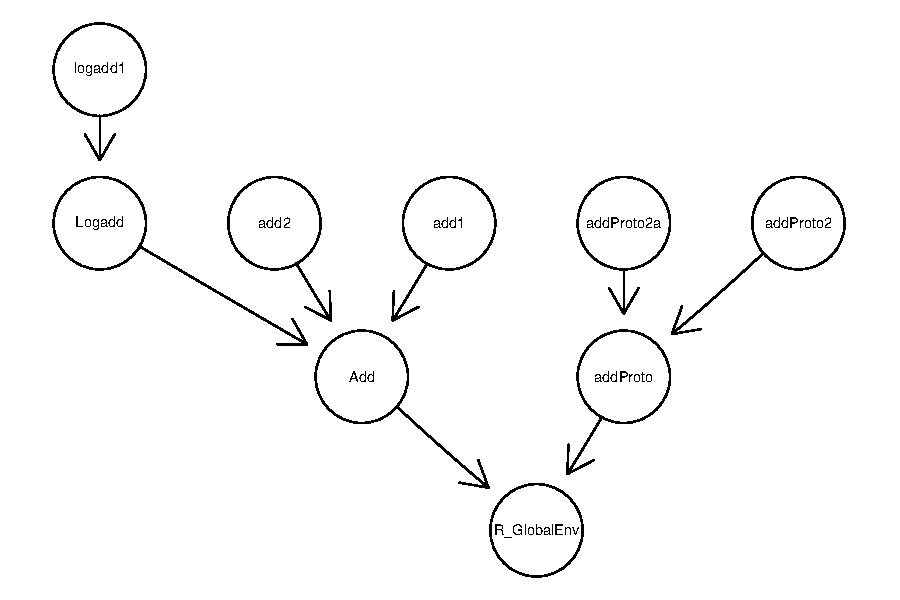
\includegraphics{proto-dot}
\caption{\label{fig:proto-dot} Ancestor tree generated using graph.proto. Edges
point from child to parent.}
\end{center}
\end{figure}

\pagebreak[4]

\section{Examples}
\label{sec:examples}

\subsection{Smoothing}
\label{sec:smooth}

In the following we create a \code{proto} object named \code{oo}
containing a vector of data \code{x} (generated from a simulated
autoregressive model) and time points
\code{tt}, an intermediate result
\code{x.smooth}, some plotting parameters \code{xlab}, \code{ylab},
\code{pch}, \code{col} and three methods \code{smooth}, \code{plot}
and \code{residuals} which smooth the data, plot the data and
calculate residuals, respectively.  We also define \code{..x.smooth}
which holds intermediate results.  Names beginning with two dots
prevent them from being delegated to children.  If we override
\code{x} in a child we would not want an out-of-sync \code{x.smooth}.
Note that the components of an object can be specified using a code
block in place of the argument notation we used previously in the
\code{proto} command.

\begin{Schunk}
\begin{Sinput}
> oo <- proto(expr = {
+     x <- rnorm(251, 0, 0.15)
+     x <- filter(x, c(1.2, -0.05, -0.18), method = "recursive")
+     x <- unclass(x[-seq(100)]) * 2 + 20
+     tt <- seq(12200, length = length(x))
+     ..x.smooth <- NA
+     xlab <- "Time (days)"
+     ylab <- "Temp (deg C)"
+     pch <- "."
+     col <- rep("black", 2)
+     smooth <- function(., ...) {
+         .$..x.smooth <- supsmu(.$tt, .$x, ...)$y
+     }
+     plot <- function(.) with(., {
+         graphics::plot(tt, x, pch = pch, xlab = xlab, ylab = ylab,
+             col = col[1])
+         if (!is.na(..x.smooth[1]))
+             lines(tt, ..x.smooth, col = col[2])
+     })
+     residuals <- function(.) with(., {
+         data.frame(t = tt, y = x - ..x.smooth)
+     })
+ })
\end{Sinput}
\end{Schunk}

Having defined our \code{proto} object we can inspect it, as shown
below, using
\code{print} which is automatically invoked if the
name of the object, \code{oo}, is entered on a line by itself.
In this case, there is no proto print method so we inherit the
environment print method which displays the environment hash code.
Although it produces too much output to show here,
we could have displayed a
list of the entire contents of the object \code{oo}
via \code{oo\$as.list(all.names = TRUE)}.
We can get a list of the names of the
components of the object using \code{oo\$ls(all.names = TRUE)} and will look
at the contents of one component, \code{oo\$pch}.

\begin{Schunk}
\begin{Sinput}
> oo
\end{Sinput}
\begin{Soutput}
<environment: 0x01fbd8c8>
attr(,"class")
[1] "proto"       "environment"
\end{Soutput}
\begin{Sinput}
> oo$ls(all.names = TRUE)
\end{Sinput}
\begin{Soutput}
 [1] "..x.smooth" ".super"     ".that"      "col"        "pch"
 [6] "plot"       "residuals"  "smooth"     "tt"         "x"
[11] "xlab"       "ylab"
\end{Soutput}
\begin{Sinput}
> oo$pch
\end{Sinput}
\begin{Soutput}
[1] "."
\end{Soutput}
\end{Schunk}

Let us illustrate a variety of manipulations.  We will set up the
output to plot 2 plots per screen using \code{mfrow}.  We change the
plotting symbol, smooth the data, invoke the \code{plot} method to
display a plot of the data and the smooth and then plot the residuals
in the second plot (figure \ref{fig:proto-smooting03}).


\begin{Schunk}
\begin{Sinput}
> par(mfrow = c(1, 2))
> oo$pch <- 20
> oo$smooth()
> oo$plot()
> plot(oo$residuals(), type = "l")
\end{Sinput}
\end{Schunk}


\begin{figure}[h!]
\begin{center}
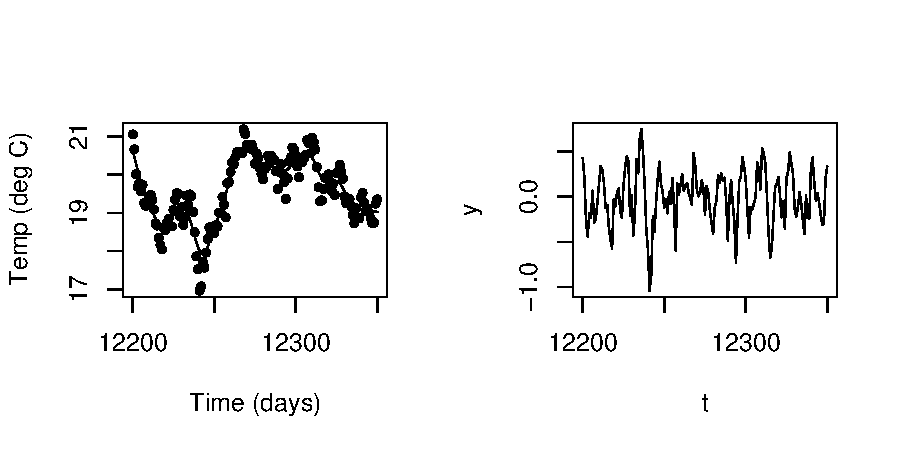
\includegraphics[width=\textwidth]{proto-smoothing03}
\end{center}
\caption{Data and smooth from \code{oo\$plot()} (left) and plot of
\code{oo\$residuals()} (right).}
\label{fig:proto-smooting03}
\end{figure}


Now let us illustrate the creation of a child object and delegation.
We create a new child object of \code{oo} called \code{oo.res}.  We
will override the \code{x} value in its parent by setting \code{x} in
the child to the value of the residuals in the parent.  We will also
override the \code{pch} and \code{ylab} plotting parameters.  We will
return to 1 plot per screen and run \code{plot} using the
\code{oo.res} object as the receiver invoking the \code{smooth} and
\code{plot} methods (which are delegated from the parent \code{oo})
with the data in the child (figure \ref{fig:smoothing04}).

\begin{Schunk}
\begin{Sinput}
> oo.res <- oo$proto(pch = "-", x = oo$residuals()$y, ylab = "Residuals deg K")
> par(mfrow = c(1, 1))
> oo.res$smooth()
> oo.res$plot()
\end{Sinput}
\end{Schunk}

% \begin{figure}[tp]
\begin{figure}[h!]
\begin{center}
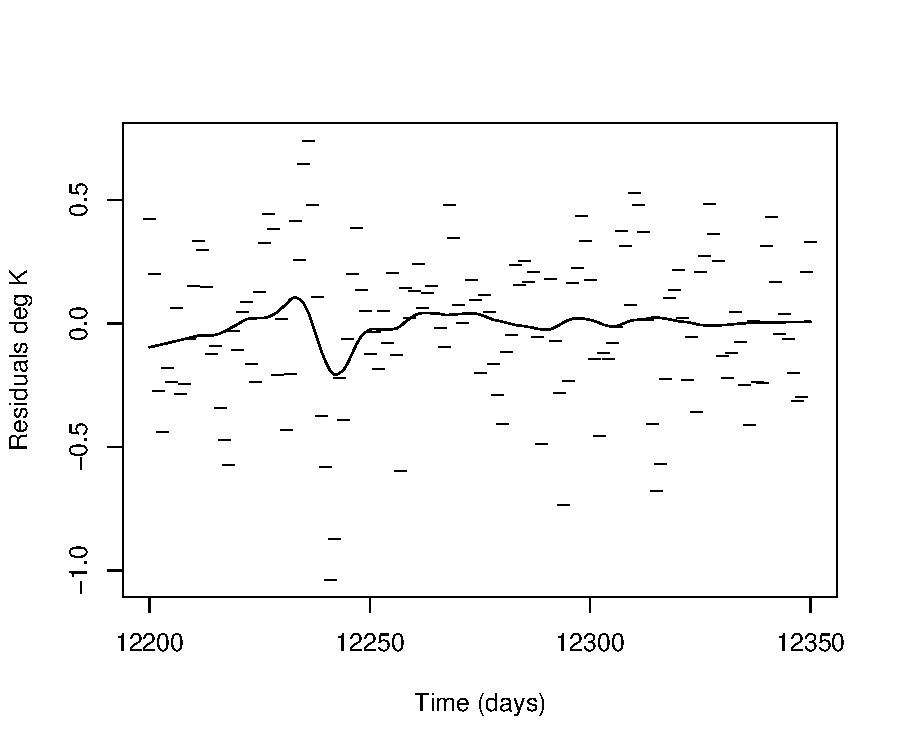
\includegraphics[width=\half]{proto-smoothing04}
\end{center}
\caption{Output of \code{oo.res\$plot()}.
\code{oo.res\$x} contains the residuals from \code{oo}.}
\label{fig:smoothing04}
\end{figure}
Now we make use of delegation to change the parent
and child in a consistent way with respect to certain plot characteristics.
We have been using a numeric time axis.
Let us interpret these numbers as the number of days since the Epoch,
January 1, 1970, and let us also change the plot colors.

\begin{Schunk}
\begin{Sinput}
> oo$tt <- oo$tt + as.Date("1970-01-01")
> oo$xlab <- format(oo.res$tt[1], "%Y")
> oo$col <- c("blue", "red")
\end{Sinput}
\end{Schunk}


We can introduce a new method, \code{splot}, into
the parent \code{oo} and have it automatically
inherited by its children.  In this example
it smooths and then plots and we use it with
both \code{oo} and \code{oo.res} (figure \ref{fig:smoothing06}).


\begin{Schunk}
\begin{Sinput}
> oo$splot <- function(., ...) {
+     .$smooth(...)
+     .$plot()
+ }
> par(mfrow = c(1, 2))
> oo$splot(bass = 2)
> oo.res$splot()
\end{Sinput}
\end{Schunk}


\begin{figure}[tbp]
\begin{center}
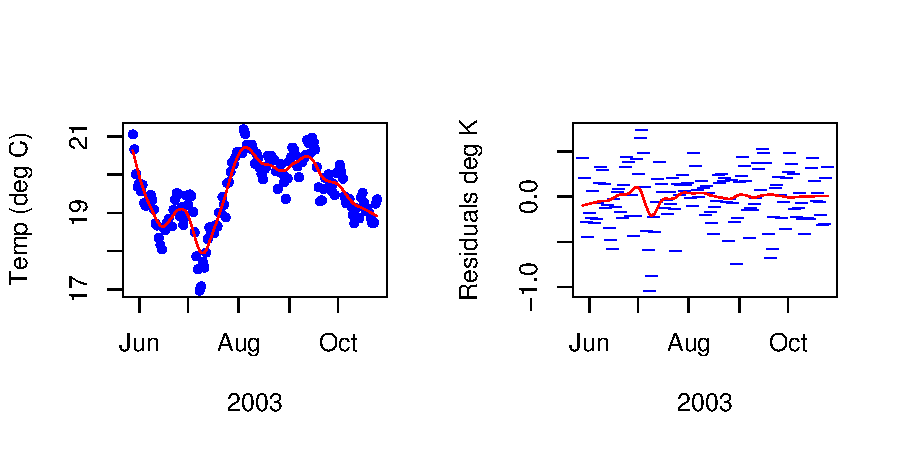
\includegraphics[width=\textwidth]{proto-smoothing06}
\caption{Plotting options and \code{splot} function applied
to both parent (left) and child (right) object}
\label{fig:smoothing06}
\end{center}
\end{figure}

Numerous possibilities exist to make use of the
mechanisms shown, so one may create different child objects, apply
different smoothing parameters, overwrite the smoothing function with
a lowess smoother and finally compare fits and residuals.

Now lets change the data and repeat the analysis.  Rather than
overwrite the data we will preserve it in \code{oo} and create a child
\code{oos} to hold an analysis with sinusoidal data.

\begin{Schunk}
\begin{Sinput}
> oos <- oo$proto(expr = {
+     tt <- seq(0, 4 * pi, length = 1000)
+     x <- sin(tt) + rnorm(tt, 0, 0.2)
+ })
> oos$splot()
\end{Sinput}
\end{Schunk}

Lets perform the residual analysis with \code{oos}.
We will make a deep copy of \code{oo.res}, i.e. duplicate its
contents and not merely delegate it, by copying \code{oo.res}
to a list from which we create the duplicate, or cloned,
\code{proto} object (figure \ref{fig:smoothing10} and \ref{fig:cloning}):

\begin{Schunk}
\begin{Sinput}
> oos.res <- as.proto(oo.res$as.list(), parent = oos)
> oos.res$x <- oos$residuals()$y
> oos.res$splot()
\end{Sinput}
\end{Schunk}


\begin{figure}[tbp]
\begin{center}
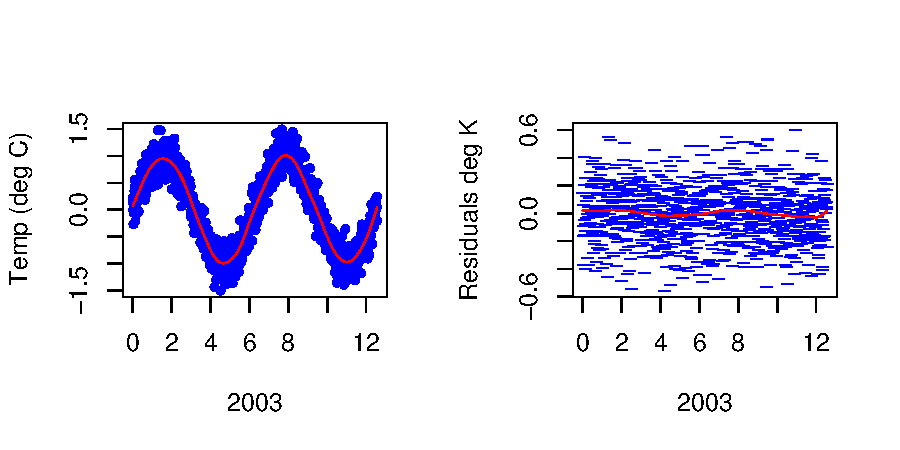
\includegraphics[width=\textwidth]{proto-smoothing10}
\caption{Smoothing of sinusoidal data (left)
and of their residuals (right)}\label{fig:smoothing10}
\end{center}
\end{figure}

\begin{figure}[h!]
\begin{center}
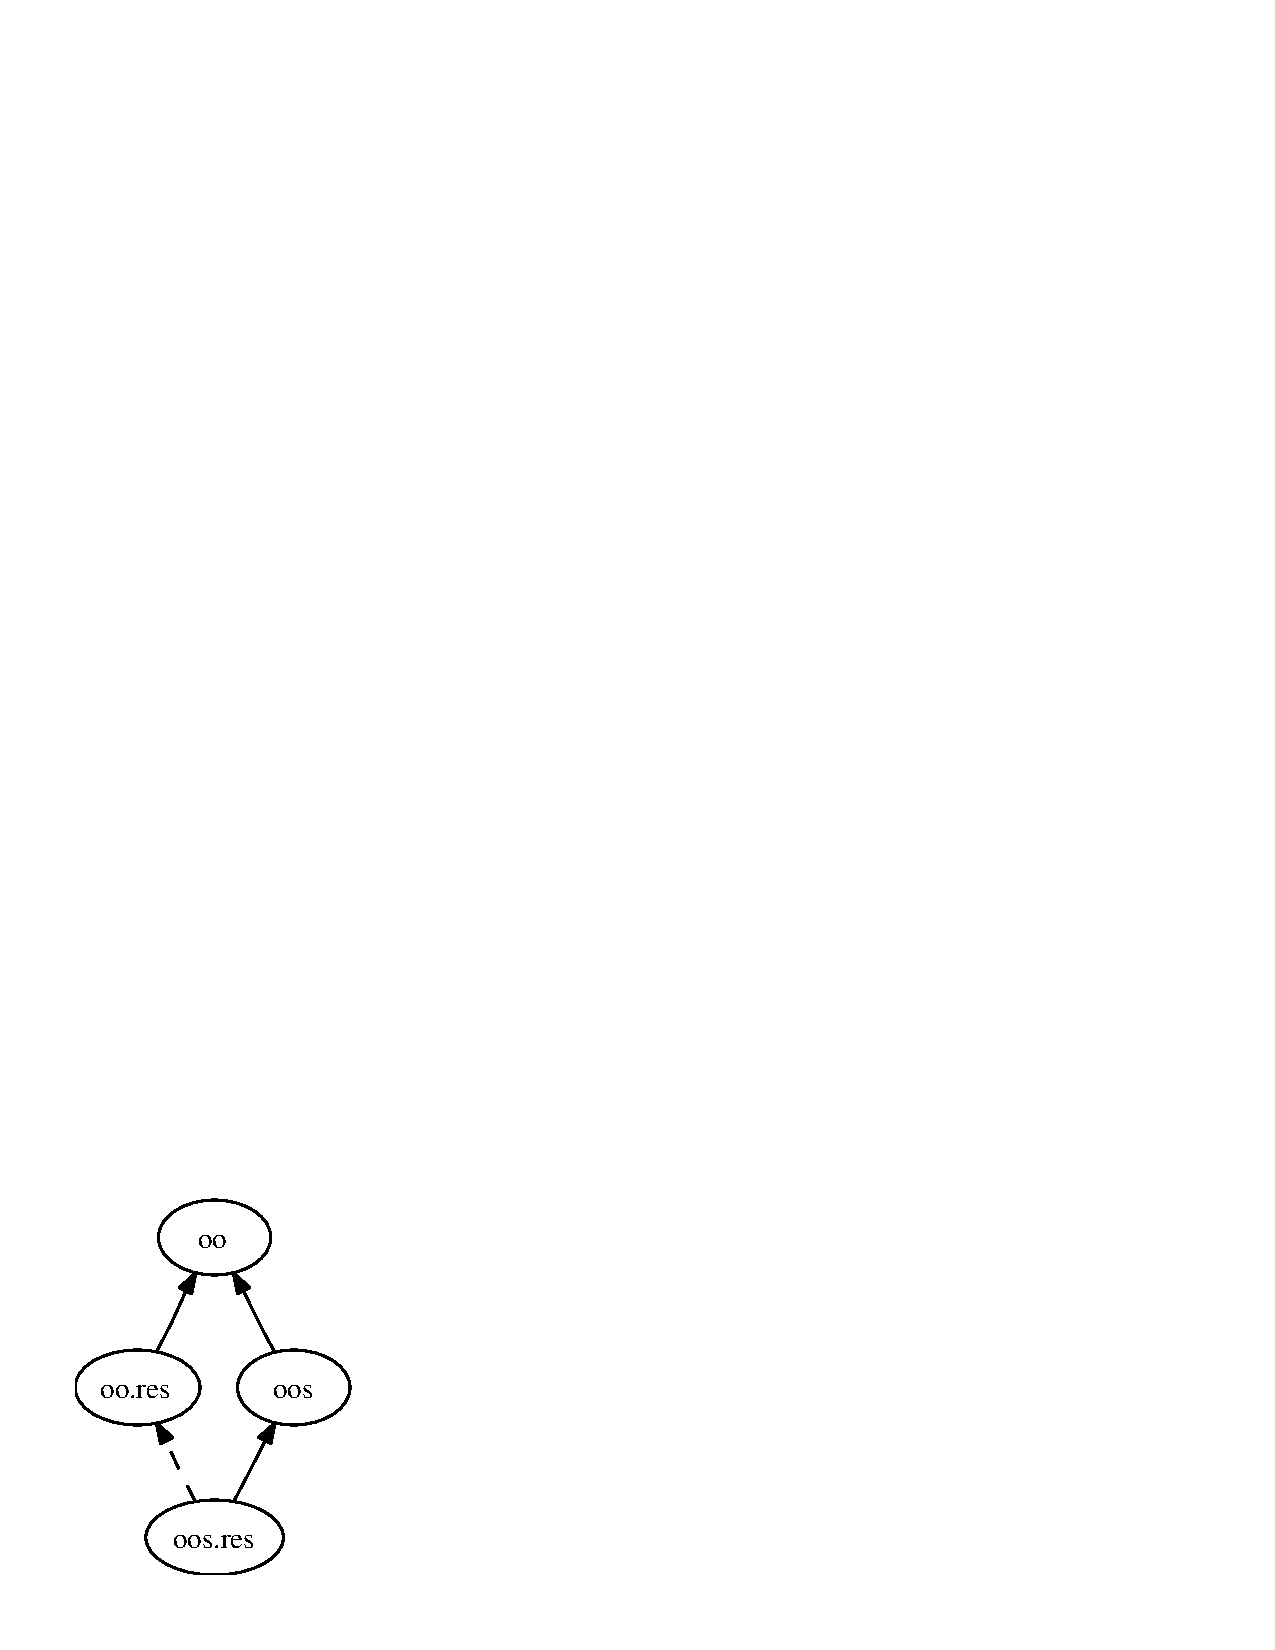
\includegraphics[width=50mm]{cloning3.pdf}
\caption{Cloning (dashed line) and delegation (solid line).  Edges point
from child to parent.}\label{fig:cloning}
\end{center}
\end{figure}

We have delegated variables
and methods and overridden both.
Thus, even with such a simple analysis, object orientation
and delegation came into play.
The reader can plainly see that smoothing and residual
analysis were not crucial to the example and this example
could be replaced with any statistical analysis including
likelihood or other estimation techniques, time series, survival
analysis, stochastic processes and so on.  The key aspect is
just that we are performing one-of analyses and do not want to
set up an elaborate class infrastructure but just want to
directly create objects to organize our calculations while
relying on delegation and dispatch to eliminate redundancy.

\subsection{Correlation, Fisher's Transform and Bootstrapping}
\label{sec:corr}

The common approach to
confidence intervals for the correlation coefficient is to
assume normality of the underlying data and then use Fisher's transform
to transform the correlation coefficient to an approximately normal
random variable.
Fisher showed that with the above normality assumption, transforming
the correlation coefficient using
the hyperbolic arc tangent function
yields a random variable
approximately distributed with an
$\frac{N(p, 1)}{\sqrt(n-3)}$ distribution.  The transformed random
variable can be used to create normal distribution confidence intervals
and the procedure can be back transformed to get confidence intervals
for the original correlation coefficient.

A more recent approach to confidence intervals for the correlation
coefficient is to use bootstrapping.  This does not require the
assumption of normality of the underlying distribution and requires
no special purpose theory devoted solely to the correlation coefficient,

Let us calculate the 95\%
confidence intervals using Fisher's transform
first.  We use \code{GNP} and \code{Unemployed} from the Longley data
set.  First we retrieve the data set and extract the required columns
into \code{x}.  Then we set \code{n} to the number of cases
and \code{pp} to the percentiles
of interest.  Finally we calculate the sample correlation and
create a function to calculate the confidence interval using
Fisher's Transform.  This function not only returns the confidence
interval but also stores it in \code{CI} in the receiver object.

\begin{Schunk}
\begin{Sinput}
> longley.ci <- proto(expr = {
+     data(longley)
+     x <- longley[, c("GNP", "Unemployed")]
+     n <- nrow(x)
+     pp <- c(0.025, 0.975)
+     corx <- cor(x)[1, 2]
+     ci <- function(.) (.$CI <- tanh(atanh(.$corx) + qnorm(.$pp)/sqrt(.$n -
+         3)))
+ })
\end{Sinput}
\end{Schunk}

Now let us repeat this analysis using the bootstrapping approach.  We
derive a new object \code{longley.ci.boot} as child of
\code{longley.ci}, setting the number of replications, \code{N}, and
defining the procedure, \code{ci} which does the actual bootstrap
calculation.

\begin{Schunk}
\begin{Sinput}
> longley.ci.boot <- longley.ci$proto({
+     N <- 1000
+     ci <- function(.) {
+         corx <- function(idx) cor(.$x[idx, ])[1, 2]
+         samp <- replicate(.$N, corx(sample(.$n, replace = TRUE)))
+         (.$CI <- quantile(samp, .$pp))
+     }
+ })
\end{Sinput}
\end{Schunk}

In the example code below the first line runs the Fisher Transform
procedure and the second runs the bootstrap procedure.  Just to check
that we have performed sufficient bootstrap iterations we rerun it in
the third line, creating a delegated object on-the-fly running its
\code{ci} method and then immediately throwing the object away.
The fact that 4,000
replications give roughly the same result as 1,000 replications
satisfies us that we have used a sufficient number of replications.

\begin{Schunk}
\begin{Sinput}
> longley.ci$ci()
\end{Sinput}
\begin{Soutput}
[1] 0.1549766 0.8464304
\end{Soutput}
\begin{Sinput}
> longley.ci.boot$ci()
\end{Sinput}
\begin{Soutput}
     2.5%     97.5%
0.2299395 0.8211854
\end{Soutput}
\begin{Sinput}
> longley.ci.boot$proto(N = 4000)$ci()
\end{Sinput}
\begin{Soutput}
     2.5%     97.5%
0.2480999 0.8259276
\end{Soutput}
\end{Schunk}

We now have the results stored in two objects nicely organized for the
future.  Note, again, that despite the simplicity of the example we
have used the features of object oriented programming, coupling the
data and methods that go together, while relying on delegation and
dispatch to avoid duplication.

\subsection{Dendrograms}
\label{sec:tree}

In \cite{Gentleman2002} there is an \proglang{S4}
example of creating a binary tree
for use as a dendrogram.  Here we directly define a binary tree with no
setup at all.  To keep it short we will create a binary tree of only
two nodes having a root whose left branch points to a leaf.  The leaf
inherits the \code{value} and \code{incr} components from the root.
The attractive feature is that the leaf be defined as a child of the
parent using \code{proto} before the parent is even finished
being defined.  Compared to the cited \proglang{S4} example where it
was necessary to create an extra class to introduce the required level of
indirection there is no need to take any similar action.

\code{tree} is the root node of the tree.  It has four components.  A
method \code{incr} which increments the \code{value} component, a
\code{..Name}, the \code{value} component itself and the left branch
\code{..left}.  \code{..left} is itself a proto object which is a
child of \code{tree}.  The leaf inherits the \code{value} component
from its parent, the root.  As mentioned, at the time we define
\code{..left} we have not even finished defining \code{tree} yet we
are able to implicitly reference the yet to be defined parent.

\begin{Schunk}
\begin{Sinput}
> tree <- proto(expr = {
+     incr <- function(., val) .$value <- .$value + val
+     ..Name <- "root"
+     value <- 3
+     ..left <- proto(expr = {
+         ..Name = "leaf"
+     })
+ })
\end{Sinput}
\end{Schunk}

Although this is a simple structure we could have embedded additional
children into \code{root} and \code{leaf} and so on recursively making
the tree or dendrogram arbitrarily complex.

Let us do some computation with this structure.  We display the
\code{value} fields in the two nodes, increment the value field in the
root and then display the two nodes again to show .that the leaf
changed too.

\begin{Schunk}
\begin{Sinput}
> cat("root:", tree$value, "leaf:", tree$..left$value, "\n")
\end{Sinput}
\begin{Soutput}
root: 3 leaf: 3
\end{Soutput}
\begin{Sinput}
> tree$incr(1)
> cat("root:", tree$value, "leaf:", tree$..left$value, "\n")
\end{Sinput}
\begin{Soutput}
root: 4 leaf: 4
\end{Soutput}
\end{Schunk}

If we increment \code{value} in \code{leaf} directly (see the example
below where we increment it by 10) then it receives its own copy of
\code{value} so from that point on \code{leaf} no longer inherits
\code{value} from \code{root}.  Thus incrementing the root by 5 no
longer increments the \code{value} field in the leaf.

\begin{Schunk}
\begin{Sinput}
> tree$..left$incr(10)
> cat("root:", tree$value, "leaf:", tree$..left$value, "\n")
\end{Sinput}
\begin{Soutput}
root: 4 leaf: 14
\end{Soutput}
\begin{Sinput}
> tree$incr(5)
> cat("root:", tree$value, "leaf:", tree$..left$value, "\n")
\end{Sinput}
\begin{Soutput}
root: 9 leaf: 14
\end{Soutput}
\end{Schunk}

\subsection{From Prototypes to Classes}
\label{sec:increment}

In many cases we will use \pkg{proto} for a design that uses prototypes
during the full development cycle.  In other cases we may use it in an
incremental way starting with prototypes but ultimately transitioning
to classes.
As shown in Section~\ref{sec:traits} the \pkg{proto} package is
powerful enough to handle class-based as well as class-free programming.
Here we illustrate this process of incremental design
starting with
concrete objects and then over time classifing them into classes,
evolving a class-based program.  \pkg{proto} provides a smooth
transition path since it can handle both the class-free and the class-based
phases -- there is no need to switch object systems part way through.
In this example, we define an object which holds a linear equation, \code{eq},
represented as a character string in terms of the unknown variable \code{x}
and a \code{print} and a \code{solve} method.  We execute the
\code{print} method
to solve it.  We also create child object \code{lineq2}
which overrides \code{eq} and execute its \code{print} method.

\begin{Schunk}
\begin{Sinput}
> lineq <- proto(eq = "6*x + 12 - 10*x/4 = 2*x", solve = function(.) {
+     e <- eval(parse(text = paste(sub("=", "-(", .$eq), ")")),
+         list(x = 0+1i))
+     -Re(e)/Im(e)
+ }, print = function(.) cat("Equation:", .$eq, "Solution:", .$solve(),
+     "\n"))
> lineq$print()
\end{Sinput}
\begin{Soutput}
Equation: 6*x + 12 - 10*x/4 = 2*x Solution: -8
\end{Soutput}
\begin{Sinput}
> lineq2 <- lineq$proto(eq = "2*x = 7*x-12+x")
> lineq2$print()
\end{Sinput}
\begin{Soutput}
Equation: 2*x = 7*x-12+x Solution: 2
\end{Soutput}
\end{Schunk}

We could continue with enhancements but at this point we decide that we
have a general case and so wish
to abstract \code{lineq} into a class.  Thus we define a trait,
\code{Lineq}, which is just \code{lineq} minus \code{eq} plus
a constructor \code{new}.  The key difference between \code{new}
and the usual \code{proto} function
is that with \code{new} the initialization of \code{eq} is mandatory.
Having completed this definition
we instantiate an object of
class/trait \code{Lineq} and execute it.

\begin{Schunk}
\begin{Sinput}
> Lineq <- lineq
> rm(eq, envir = Lineq)
> Lineq$new <- function(., eq) proto(., eq = eq)
> lineq3 <- Lineq$new("3*x=6")
> lineq3$print()
\end{Sinput}
\begin{Soutput}
Equation: 3*x=6 Solution: 2
\end{Soutput}
\end{Schunk}

Note how we have transitioned from a prototype style of programming
to a class-based style of programming all the while staying within
the \pkg{proto} framework.

\section{Summary} \label{sec:summary}

\subsection{Benefits}
\label{sec:benefits}

The key benefit of the \pkg{proto} package is to provide
access to a style of programming that has not been conveniently
accessible within \proglang{R} or any other mainstream language today.

\pkg{proto} can be used in two key ways: class-free object oriented programming
and class-based object oriented programming.

A key application for \pkg{proto} in class-free programming is to wrap the code
and data for each run of a particular statistical study into an object for
purposes of organization and reproducibility.  It provides such organization
directly and without the need and overhead of class definitions
yet still provides the
inheritance and dispatch advantages of object oriented programming.
We provide examples of this style of programming in
Section~\ref{sec:smooth}
and
Section~\ref{sec:corr}.
A third example in
Section~\ref{sec:tree} illustrates a beneficial use of \pkg{proto} with
recursive data structures.

Another situation where prototype programming is of interest is in the initial
development stages of a program.  In this case, the design may not be fully
clear so it is more convenient to create concrete objects individually rather
than premature abstractions through classes.  The \code{graph.proto}
function can be used to generate visual representations of the object
tree suggesting classifications of objects so that
as the program evolves the general case becomes clearer and
in a bottom up fashion the objects are incrementally abstracted into
classes.  In this case,
\pkg{proto} provides a smooth transition path since it not only supports
class-free programming but, as explained in the Section~\ref{sec:traits}, is
sufficiently powerful to support class-based programming, as well.


\subsection{Conclusion}
\label{sec:conclusion}

The package \pkg{proto} provides an \proglang{S3} subclass of the
\code{environment} class for constructing and manipulating object
oriented systems without classes.  It can also emulate classes even
though classes are not a primitive structure.  Its key design goals
are to provide as simple and as thin a layer as practically possible
while giving the user convenient access to this alternate object
oriented paradigm.  This paper describes, by example, how prototype
programming can be carried out in \proglang{R} using \pkg{proto} and
illustrates such usage.  Delegation, cloning traits and general
manipulation and incremental development are all reviewed by example.

\section*{Computational details}
\label{sec:compute}

The results in this paper were obtained using \proglang{R} 2.1.0 with
the package \pkg{proto} 0.3--2. \proglang{R} itself and the
\pkg{proto} package are available from CRAN at
\url{http://CRAN.R-project.org/}.  The GraphViz software is available
from \url{http://www.graphviz.org}.

\phantomsection
\addcontentsline{toc}{section}{References}
\bibliography{proto}
%

%\VignetteIndexEntry{proto: An R Package for Prototype Programming}
%\VignetteDepends{}
%\VignetteKeywords{object oriented, prototype programming, S3, R}
%\VignettePackage{proto}


\documentclass[nojss]{jss}
\usepackage{Sweave}
\DeclareGraphicsExtensions{.pdf, .eps, .png}



\newlength{\half}
\setlength{\half}{70mm}

\author{Louis Kates\\GKX Associates Inc. \And
        Thomas Petzoldt\\Technische Universit\"at Dresden}
\Plainauthor{Louis Kates, Thomas Petzoldt}

\title{\pkg{proto}: An \proglang{R} Package for Prototype Programming}
%% \Shorttitle{\pkg{proto}: An \proglang{R} Package for Prototype Programming}

\Plaintitle{proto: An R Package for Prototype Programming}

\Keywords{prototype programming, delegation, inheritance, clone,
  object orientated, \proglang{S3}, \proglang{R}}
\Plainkeywords{object oriented, prototype programming, S3, R}

\Abstract{

  \pkg{proto} is an \proglang{R} package which facilitates a style
  of programming known as prototype
  programming.  Prototype programming is a type of object
  oriented programming in which there are no classes.
  \pkg{proto} is simple yet retains the object oriented features of
  delegation (the prototype counterpart to inheritance)
  and object oriented  dispatch.  \code{proto} can be used
  to organize the concrete data and procedures in statistical studies
  and other applications
  without the necessity of defining classes while still providing convenient
  access to an object oriented style of programming.  Furthermore, it
  can be used in a class-based style as well so that incremental design can
  begin with defining the concrete objects and later transition to abstract
  classes, once the general case is understood, without having to change to
  object-oriented frameworks.
  The key goals of the package are to integrate into \proglang{R}
  while providing nothing more than a thin layer on top of it.
}

\hyphenation{ma-ni-pu-lating}

\begin{document}
\Sconcordance{concordance:proto.tex:proto.Rnw:%
1 1362 1}





\section{Introduction} \label{sec:intro}

\subsection[Object Oriented Programming in R]{Object Oriented Programming in \proglang{R}}
\label{sec:oo}

The \proglang{R} system for statistical computing
\citep[\url{http://www.R-project.org/}]{Rcore2005} ships with two
systems for object oriented programming referred to as \proglang{S3}
and \proglang{S4}.  With the increased interest in object oriented
programming within \proglang{R} over the last years additional object
oriented programming packages emerged.  These include the \pkg{R.oo}
package \citep{Bengtsson2003} and the \pkg{OOP} package
\citep[\url{http://www.omegahat.net/OOP/}]{Rnews:Chambers+Lang:2001a}.
All these packages have the common thread that they use
classes as the basis of inheritance.  When a message is sent to an
object the class of the object is examined and that class determines the
specific function to be executed. In prototype programming there
are no classes making it simple yet it retains much of the power of
class-based programming.  In the fact, \pkg{proto} is so simple that
there is only one significant new routine name, \code{proto}.  The
other routines are just the expected support routines such as
\code{as.proto} to coerce objects to proto objects, \code{\$} to
access and set proto object components and \code{is.proto} to check
whether an object is a proto object.  In addition, \code{graph.proto}
will generate a graphical ancestor tree showing the parent-child
relationships among generated \code{proto} objects.

The aim of the package is to provide a lightweight layer for prototype
programming in \proglang{R} written only in \proglang{R} leveraging the
existing facilities of the language rather than adding its own.

\subsection{History}
\label{sec:history}

The concept of
prototype programming
\citep{Lieberman1986, Taivalsaari1996a, Noble1999}
has developed over a number of years with the \proglang{Self}
language \citep{Agesen1992}
being the key evolved programming language to demonstrate
the concept.  In statistics, the \proglang{Lisp}-based
\proglang{LispStat} programming language \citep{Tierney1990} was
the first and possibly only statistical system to feature prototype
programming.

Despite having been developed over 20 years ago, and some attempts to
enter the mainstream (e.g.  \proglang{Newtonscript}
on the Newton computer, which
is no longer available, and \proglang{Javascript} where
it is available but whose
domain of application largely precluses use of prototype programming)
prototype programming is not well known due to lack of language
support in popular programming languages such as \proglang{C} and
\proglang{Java}.  It tends
to be the domain of research languages or \proglang{Lisp}.

Thus the
the availability of a popular language,
\proglang{R} \footnote{Some indications of the popularity of R are
the high volume mailing lists, international development team, the
existence of over 500 addon packages, conferences and numerous books
and papers devoted to R.},
that finally does provide the key infrastructure
is an important development.

This work grew out of the need to organize multiple scenarios of model
simulations in ecological modelling \citep{Rnews:Petzoldt:2003} and
was subsequently generalized to the present package.  A number of
iterations of the code, some motivated by the ever increasing feature
set in \proglang{R}, resulted in a series of utilities and ultimately
successive versions of an \proglang{R} package developed over the last
year.  An initial version used \proglang{R} lists as the basis of the
package.  Subsequently the package was changed to use \proglang{R}
environments.  The first version to use environments stored the
receiver object variable in a proxy parent environment which was
created on-the-fly at each method call.  The present version of
the \pkg{proto} package passes the receiver object through the argument list,
while hiding this from the caller.  It defines the \code{proto} class
as a subclass of the \code{environment} class so that
functionality built into \proglang{R} for the environment class is
automatically inherited by the \code{proto} class.

\subsection{Overview}
\label{sec:overview}

It is assumed that the reader has some general
familiarity with object oriented programming concepts and with
\proglang{R}.

The paper will proceed primarily by example focusing on illustrating
the package \code{proto} through such demonstration.  The remainder of
the paper is organized as follows: Section~\ref{sec:proto-class}
explains how \code{"proto"} objects are created and illustrates the
corresponding methods for setting and getting components.  It further
discusses how object oriented delegation (the prototype programming
analogue of inheritance) is handled and finally discusses the
internals of the package.  This section uses small examples chosen for
their simplicity in illustrating the concepts.  In
Section~\ref{sec:examples} we provide additional examples of prototype
programming in action.  Four examples are shown.  The first involves
smoothing of data.  Secondly we demonstrate the calculation of
correlation confidence intervals using classical (Fisher Transform)
and modern (bootstrapping) methods.  Thirdly we demonstrate the
development of a binary tree as would be required for a dendrogram.
Fourthly, we use the solution of linear equations to illustrate
program evolution from object-based to class-based, all
within the \pkg{proto} framework.
Section~\ref{sec:summary} gives a few summarizing remarks.  Finally,
an appendix provides a reference card that summarizes the
functionality contained in \pkg{proto} in terms of its constituent
commands.

%% \pagebreak[4]

\section[The class "proto" and its methods]{The class \code{"proto"} and its methods}
\label{sec:proto-class}

\subsection[Creation of "proto" objects]{Creation of \code{"proto"} objects}
\label{sec:proto}

In this section we shall show, by example, the creation of two
prototype objects and related operations.  The simple idea is that
each \code{"proto"} object is a set of components: functions (methods)
and variables, which are tightly related in some way.

A prototype object is an environment holding the variables and
methods of the object. \footnote{In particular this implies that
\code{"proto"} objects have single inheritance, follow ordinary
environment scoping rules and have mutable state as environments
do.}

A prototype object is created using the constructor function
\code{proto} (see Appendix~\ref{sec:ref} at the end of this paper or
\pkg{proto} package help for complete syntax of commands).

\begin{Scode}
addProto <- proto( x = rnorm(5), add = function(.) sum(.$x) )
\end{Scode}

In this simple example, the \code{proto} function defines two
components: a variable \code{x} and a method \code{add}.  The variable
\code{x} is a vector of 5 numbers and the method sums those numbers.
The \code{proto} object \code{addProto} contains the variable and the
method.  Thus the \code{addProto} \code{proto} object can be used to compute
the sum of the values stored in it.
As shown with the \code{add} method in this example, formal argument
lists of methods must always have a first argument of dot
(i.e. \code{.})  which signifies the object on which the method is
operating.  The dot refers to the current object in the same way that
a dot refers to the current directory in UNIX.  Within the method one
must refer to other variables and methods in the object by prefacing
each with \code{.\$}.  For example, in the above we write
\code{sum(.\$x)}.  Finally, note that the data and the method are very
closely related.  Such close coupling is important in order to create
an easily maintained system.

To illustrate the usage of \code{proto}, we first load the package and
set the random seed to make the examples in this paper exactly
reproducible.

\begin{Schunk}
\begin{Sinput}
> library(proto)
> set.seed(123)
\end{Sinput}
\end{Schunk}

Then, we create the \code{proto} object from above
and call its \code{add} method.
\begin{Schunk}
\begin{Sinput}
> addProto <- proto(x = rnorm(5), add = function(.) sum(.$x))
> addProto$add()
\end{Sinput}
\begin{Soutput}
[1] 0.9678513
\end{Soutput}
\end{Schunk}
We also create another object, \code{addProto2}
with a different \code{x} vector and
invoke its \code{add} method too.
\begin{Schunk}
\begin{Sinput}
> addProto2 <- addProto$proto(x = 1:5)
> addProto2$add()
\end{Sinput}
\begin{Soutput}
[1] 15
\end{Soutput}
\end{Schunk}
In the examples above, we created a prototype object \code{addProto}
and then called its \code{add} method as just explained.
The notation \code{addProto\$add}
tells the system to look for the \code{add} method
in the \code{addProto} object.  In the expression \code{addProto\$add},
the \code{proto} object to the left
of the dollar sign, \code{addProto} here, is referred to as the
\emph{receiver} object.  This expression
also has a second purpose which is to
pass the receiver object implicitly as the first argument of \code{add}.
Note that we called \code{add} as if it had zero arguments but, in fact,
it has one argument because the receiver is automatically and implicitly
supplied as the first argument.  In general,
the notation \code{object\$method(arguments)} is
used to invoke the indicated method of the receiver object using the
object as the implicit first argument along with the indicated
arguments as the subsequent arguments.
As with the \code{addProto} example, the receiver
object not only determines where to find the
method but also is implicitly passed to the method through
the first argument.  The motivation for this notation
is to relieve the user of
specifying the receiver object twice:
once to locate the method in the object and a second
time to pass the object itself to the method.
The \code{\$} is overloaded by the \code{proto}
class to automatically do both with one reference to the receiver object.
Even though, as with the \code{addProto} example, the first
argument is not listed in the call
it still must be listed among the formal arguments
in the definition of the method.  It
is conventional to use
a dot \code{.} as the first formal argument in the method/function
definition.  That is, we call \code{add} using \code{addProto\$add()}
displaying zero arguments
but we define \code{add} in \code{addProto} displaying
one argument \code{add <- function(.)}, the dot.

In this example,
we also created a second object, \code{addProto2},
which has the first object, \code{addProto} as its parent.
Any reference to a
component in the second object that is unsuccessful will cause
search to continue in the parent.  Thus the call \code{addProto2\$add()}
looks for \code{add} in \code{addProto2} and not finding it there
searches its parent, \code{addProto}, where it is, indeed, found.
\code{add} is invoked with the receiver object, \code{addProto2}, as
the value of dot.
The call \code{addProto2\$add()} actually causes the \code{add}
in \code{addProto} to run but it still uses the \code{x} from
\code{addProto2} since dot (\code{.}) is \code{addProto2} here
and \code{add} references \code{.\$x}.
Note that the reference to \code{.\$x} in the
\code{add} found in \code{addProto}
does not refer to the \code{x} in \code{addProto} itself.
The \code{x} in \code{addProto2} has overridden the \code{x} in its parent.
This point is important so the reader should take care to absorb this
point.

This simple example already shows the key elements of the system
and how \emph{delegation} (the prototype programming term for inheritance)
works without classes.

We can add new components or replace components in an object and
invoke various methods like this:
\begin{Schunk}
\begin{Sinput}
> addProto2$y <- seq(2, 10, 2)
> addProto2$x <- 1:10
> addProto2$add3 <- function(., z) sum(.$x) + sum(.$y) + sum(z)
> addProto2$add()
\end{Sinput}
\begin{Soutput}
[1] 55
\end{Soutput}
\begin{Sinput}
> addProto2$add3(c(2, 3, 5))
\end{Sinput}
\begin{Soutput}
[1] 95
\end{Soutput}
\begin{Sinput}
> addProto2$y
\end{Sinput}
\begin{Soutput}
[1]  2  4  6  8 10
\end{Soutput}
\end{Schunk}

In this example, we insert variable \code{y} into the object \code{addProto2}
with a value of \code{seq(2,10,2)},
reset variable \code{x} to a new value and insert a new method,
\code{add3}. Then we invoke
our two methods and display \code{y}.  Again, note that in the case of
\code{protoAdd2\$add} the \code{add} method is not present in
\code{protoAdd2} and so search continues to the parent \code{addProto}
where it is found.

\subsection{Internals}
\label{sec:internals}

So far, we have used simple examples to illustrate the basic manipulation
of objects: construction, getting and setting components and method
invocation.  We now discuss the internals of the package and how it relates
to \proglang{R} constructs.
\code{proto} is actually an \proglang{S3} class which is a subclass
of the \code{environment} class.  Every \code{proto} object is an
environment and its class is \code{c("proto", "environment")}.  The \code{\$}
accessor is similar to the same accessor in environments except it will
use the \proglang{R} \code{get} function to
search up parent links if it cannot otherwise find the object (unlike
environments).  When accessing a method, \code{\$}
automatically supplies the
first argument to the method
unless the object is \code{.that} or \code{.super}.  \code{.that}
is a special variable which \code{proto} adds to every \code{proto} object
denoting the object itself.  \code{.super} is also added to every
proto object and is the parent of \code{.that}.  \code{.that}
and \code{.super} are normally used
within methods of an object to refer to other components of the same
or parent object, respectively,
as opposed to the receiver (\code{.}).  For example,
suppose we want \code{add} in \code{addProto2} to add the elements
of \code{x} together and the elements of
\code{y} together and then add these two sums.  We could redefine add like this:

\begin{Schunk}
\begin{Sinput}
> addProto2$add <- function(.) .super$add(.) + sum(.$y)
\end{Sinput}
\end{Schunk}

making use of the \code{add} already defined in the parent.
One exception should be noted here.  When one uses \code{.super},
as above, or \code{.that} to specify a method then the receiver
object must be explicitly specified
in argument one (since in those cases the receiver
is possibly different than
\code{.super} or \code{.that} so the system cannot automatically supply it
to the call.)

Setting a value is similar to the corresponding operation for
environments except that any function, i.e method, which is
inserted has its environment set to the environment of the object
into which it is being inserted.  This is necessary so that such
methods can reference \code{.that} and \code{.super} using
lexical scoping.

In closing this section a few points should be re-emphasized and
expanded upon.  A
\code{proto} object is an environment whose parent object is the
parent environment of the \code{proto} object.  The methods in the \code{proto}
objects are ordinary functions that have the containing object as their
environment.

The \proglang{R} \code{with} function can be used with environments and
therefore can be used with \code{proto} objects since \code{proto}
objects are environments too.  Thus \code{with(addProto, x)} refers
to the variable \code{x} in \code{proto} object \code{addProto}
and \code{with(addProto, add)} refers to the method \code{add}
in the same way.  \code{with(addProto, add)(addProto)} can be used
to call \code{add}.  These constructs all follow from their corresponding
use in environments from which they are inherited.

Because the \code{with} expressions are somewhat verbose, two common
cases can be shortened using the \code{\$} operator.  \code{addProto\$x}
can be used to refer to variable \code{x} in \code{proto} object
\code{addProto} and has the same meaning as \code{with(addProto, x)}.
In particular like \code{with} but
unlike the the behavior of the \code{\$} operator on
environments, when used with \code{proto} objects, \code{\$} will
search not only the object itself but also its ancestors.
Similarly \code{addProto\$add()} can be used to call
method \code{add} in \code{addProto} also searching through ancestors
if not found in \code{addProto}.  Note that \code{addProto\$add}
returns an object of class

\code{c("instantiatedProtoMethod", "function")}
which is derived from \code{add} such that the first argument,
the \code{proto} object,
is already inserted.  Note that there is a \code{print} method for
class \code{"instantiatedProtoMethod"} so printing such objects will
display the underlying function but returning such objects
is not the same as returning the function without slot one inserted.
Thus, if one wants exactly the original \code{add}
as a value one should use \code{with(addProto, add)} or
\code{addProto\$with(add)}.

Within a method, if a variable is referred to without
qualification simply as \code{x}, say, then  its meaning  is
unchanged from how it is otherwise used in \proglang{R} and
follows the same scope rules as any variable to resolve its name.  If it is
desired that the variable have object scope, i.e. looked up
in the receiver object and its ancestors, then \code{.\$x}
or similar \code{with} notation, i.e. \code{with(., x)}, should be used.
Similarly \code{.\$f(x)} calls
method \code{f} automatically inserting the receiver object
into argument one and using \code{x} for argument two.  It
looks for \code{f} first in the receiver object and then its
ancestors.

\subsection{Traits}
\label{sec:traits}

Let us look at the definition of a child object once again.
In the code below,
\code{addProto} is the previously defined parent object
and the expression \code{addProto\$proto(x = 1:5)} defines
a child object of \code{addProto} and assigns it to variable
\code{addProto2a}.

\begin{Schunk}
\begin{Sinput}
> addProto2a <- addProto$proto(x = 1:5)
> addProto2a$add()
\end{Sinput}
\begin{Soutput}
[1] 15
\end{Soutput}
\end{Schunk}

That is, \code{proto} can be used to create a new child of
an existing object by writing the
parent object on the left of the \code{\$} and
\code{proto} on its right.  Any contents to
be added to the new child are listed in arguments of \code{proto}
as shown.

For example, first let us create a class-like structure.  In the
following \code{Add} is an object that behaves very much like a class
with an \code{add} method and a method \code{new} which constructs
new objects.  In the line creating object \code{add1} the expression
\code{Add\$new(x = 1:5)} invokes the \code{new} constructor of the
receiver object \code{Add}. The method \code{new} has an argument of
\code{x = 1:5} which defines an \code{x} variable in the \code{add1}
object being instantiated. We similarly create another object
\code{add2}.

\begin{Schunk}
\begin{Sinput}
> Add <- proto(add = function(.) sum(.$x), new = function(., x) .$proto(x = x))
> add1 <- Add$new(x = 1:5)
> add1$add()
\end{Sinput}
\begin{Soutput}
[1] 15
\end{Soutput}
\begin{Sinput}
> add2 <- Add$new(x = 1:10)
> add2$add()
\end{Sinput}
\begin{Soutput}
[1] 55
\end{Soutput}
\end{Schunk}

An object which contains only methods and variables that are
intended to be shared by all its children (as opposed to an
object whose purpose is to have its own methods and variables)
is known as a \emph{trait} \citep{Agesen1992}.  It
is similar to a class in class-based
object oriented programming.
Note that the objects \code{add1} and \code{add2} have the trait
\code{Add} as their parent.  We could implement subclass-like and
superclass-like objects by simply defining similar trait objects to
be the parent or child of \code{Add}.  For example, suppose we
want a class which calculates the sum of the logarithms of the data.  We
could define:

\begin{Schunk}
\begin{Sinput}
> Logadd <- Add$proto(logadd = function(.) log(.$add()))
> logadd1 <- Logadd$new(1:5)
> logadd1$logadd()
\end{Sinput}
\begin{Soutput}
[1] 2.70805
\end{Soutput}
\end{Schunk}

Here the capitalized objects are traits.
\code{Logadd} is a trait.  It is a child of \code{Add}
which is also a trait.  \code{logadd1} is an ordinary object,
not a trait.
One possible design is to create a tree of traits and other objects
in which the leaves are ordinary objects and the remaining nodes
are traits.  This would closely correspond to class-based
object oriented programming.

Note that the delegation of methods from
one trait to another as in
\code{new} which is inherited by \code{Logadd} from \code{Add}
is nothing more than the same mechanism by which traits delegate
methods to
objects since, of course, traits are just objects no different
from any other object other than by the conventions we impose on them.
This unification of subclassing and instantiation beautifully
shows the simplification that prototype programming represents.

\subsection{Utilities}
\label{sec:utilities}
The fact that method calls automatically insert the first argument
can be used to good effect in leveraging existing \proglang{R}
functions while allowing an object-oriented syntax.

For example, \code{ls()} can be used to list the components of
\code{proto} objects:

\begin{Schunk}
\begin{Sinput}
> addProto$ls()
\end{Sinput}
\begin{Soutput}
[1] "add" "x"
\end{Soutput}
\end{Schunk}

Functions like:

\begin{Schunk}
\begin{Sinput}
> addProto$str()
> addProto$print()
> addProto$as.list()
> addProto2a$parent.env()
\end{Sinput}
\end{Schunk}

show additional information about the elements.  \code{eapply}
can be used to explore more properties such as the
the length of each component of an object:

\begin{Schunk}
\begin{Sinput}
> addProto$eapply(length)
\end{Sinput}
\end{Schunk}

Another example of some interest in any object oriented system
which allows multiple references to one single object is that
object identity
can be tested using the respective base function:

\begin{Schunk}
\begin{Sinput}
> addProto$identical(addProto2)
\end{Sinput}
\begin{Soutput}
[1] FALSE
\end{Soutput}
\end{Schunk}

\code{proto} does contain a special purpose \code{str.proto} function
but in the main it
is important to notice here, that
\code{proto} has no code that is specific to \code{ls} or
any of the other ordinary \proglang{R}
functions listed.  We are simply making use of the
fact that \code{obj\$fun(...)} is transformed into \code{get("fun",
obj)(obj, ...)} by the proto \code{\$} operator.  For example, in the
case of \code{addProto\$ls()} the system looks for \code{ls} in object
\code{addProto}.  It cannot find it there so it looks to its parent,
which is the global environment.  It does not find it there so it
searches the remainder of the search path, i.e. the path shown by
running the \proglang{R} command \code{search()}, and finally finds it
in the base package, invoking it with an argument of \code{addProto}.
Since all \code{proto} objects are also environments
\code{ls(addProto)} interprets \code{addProto} as an environment and
runs the \code{ls} command with it.  In the \code{ls} example there
were no arguments other than \code{addProto}, and even that one was
implicit, but if there were
additional arguments then they would be passed as shown in the
\code{eapply} and \code{identical} examples above.

\subsection{Plotting}
\label{sec:plot}

The \code{graph.proto} function can be used to create
graphs that can be rendered by the \code{Rgraphviz} package
creating visual representations of ancestor trees (figure
\ref{fig:proto-dot}).
That package provides an interface to the
\proglang{GraphViz} \code{dot} program \citep{Ganser+North:1999}.

\code{graph.proto} takes three arguments, all of which are
usually omitted.  The first argument is a \code{proto} object
(or an environment) out of which all contained \code{proto} objects
and their parents (but not higher order ancestors) are graphed.
If it is omitted, the current environment is assumed.
The second argument is a graph (in the sense of the \code{graph}
package) to which the nodes and edges are added.  If it is omitted
an empty graph is assumed.  The last argument is a logical variable
that specifies the orientation of arrows.  If omitted arrows are
drawn from children to their parents.


\begin{Schunk}
\begin{Sinput}
> library(Rgraphviz)
> g <- graph.proto()
> plot(g)
\end{Sinput}
\end{Schunk}


\begin{figure}[htbp]
\begin{center}
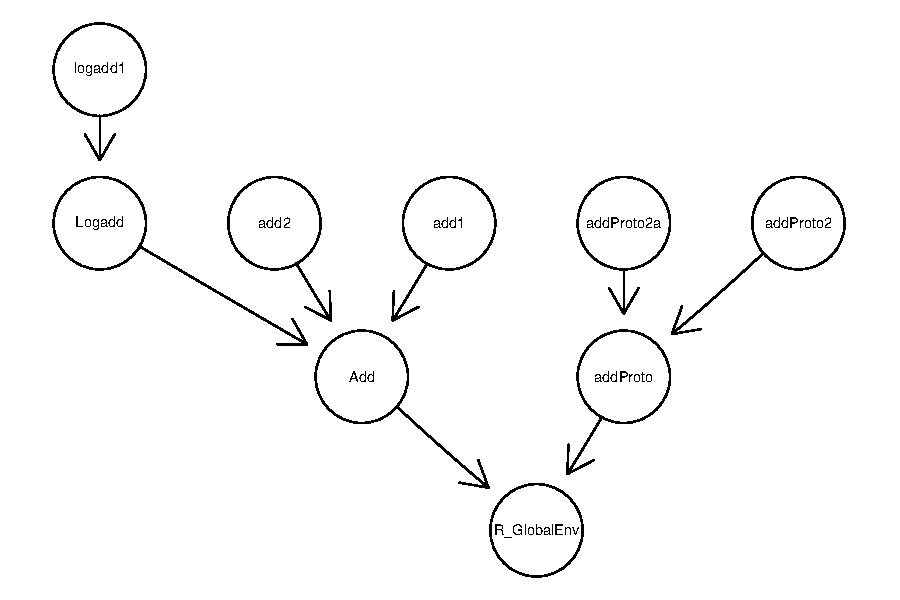
\includegraphics{proto-dot}
\caption{\label{fig:proto-dot} Ancestor tree generated using graph.proto. Edges
point from child to parent.}
\end{center}
\end{figure}

\pagebreak[4]

\section{Examples}
\label{sec:examples}

\subsection{Smoothing}
\label{sec:smooth}

In the following we create a \code{proto} object named \code{oo}
containing a vector of data \code{x} (generated from a simulated
autoregressive model) and time points
\code{tt}, an intermediate result
\code{x.smooth}, some plotting parameters \code{xlab}, \code{ylab},
\code{pch}, \code{col} and three methods \code{smooth}, \code{plot}
and \code{residuals} which smooth the data, plot the data and
calculate residuals, respectively.  We also define \code{..x.smooth}
which holds intermediate results.  Names beginning with two dots
prevent them from being delegated to children.  If we override
\code{x} in a child we would not want an out-of-sync \code{x.smooth}.
Note that the components of an object can be specified using a code
block in place of the argument notation we used previously in the
\code{proto} command.

\begin{Schunk}
\begin{Sinput}
> oo <- proto(expr = {
+     x <- rnorm(251, 0, 0.15)
+     x <- filter(x, c(1.2, -0.05, -0.18), method = "recursive")
+     x <- unclass(x[-seq(100)]) * 2 + 20
+     tt <- seq(12200, length = length(x))
+     ..x.smooth <- NA
+     xlab <- "Time (days)"
+     ylab <- "Temp (deg C)"
+     pch <- "."
+     col <- rep("black", 2)
+     smooth <- function(., ...) {
+         .$..x.smooth <- supsmu(.$tt, .$x, ...)$y
+     }
+     plot <- function(.) with(., {
+         graphics::plot(tt, x, pch = pch, xlab = xlab, ylab = ylab,
+             col = col[1])
+         if (!is.na(..x.smooth[1]))
+             lines(tt, ..x.smooth, col = col[2])
+     })
+     residuals <- function(.) with(., {
+         data.frame(t = tt, y = x - ..x.smooth)
+     })
+ })
\end{Sinput}
\end{Schunk}

Having defined our \code{proto} object we can inspect it, as shown
below, using
\code{print} which is automatically invoked if the
name of the object, \code{oo}, is entered on a line by itself.
In this case, there is no proto print method so we inherit the
environment print method which displays the environment hash code.
Although it produces too much output to show here,
we could have displayed a
list of the entire contents of the object \code{oo}
via \code{oo\$as.list(all.names = TRUE)}.
We can get a list of the names of the
components of the object using \code{oo\$ls(all.names = TRUE)} and will look
at the contents of one component, \code{oo\$pch}.

\begin{Schunk}
\begin{Sinput}
> oo
\end{Sinput}
\begin{Soutput}
<environment: 0x01fbd8c8>
attr(,"class")
[1] "proto"       "environment"
\end{Soutput}
\begin{Sinput}
> oo$ls(all.names = TRUE)
\end{Sinput}
\begin{Soutput}
 [1] "..x.smooth" ".super"     ".that"      "col"        "pch"
 [6] "plot"       "residuals"  "smooth"     "tt"         "x"
[11] "xlab"       "ylab"
\end{Soutput}
\begin{Sinput}
> oo$pch
\end{Sinput}
\begin{Soutput}
[1] "."
\end{Soutput}
\end{Schunk}

Let us illustrate a variety of manipulations.  We will set up the
output to plot 2 plots per screen using \code{mfrow}.  We change the
plotting symbol, smooth the data, invoke the \code{plot} method to
display a plot of the data and the smooth and then plot the residuals
in the second plot (figure \ref{fig:proto-smooting03}).


\begin{Schunk}
\begin{Sinput}
> par(mfrow = c(1, 2))
> oo$pch <- 20
> oo$smooth()
> oo$plot()
> plot(oo$residuals(), type = "l")
\end{Sinput}
\end{Schunk}


\begin{figure}[h!]
\begin{center}
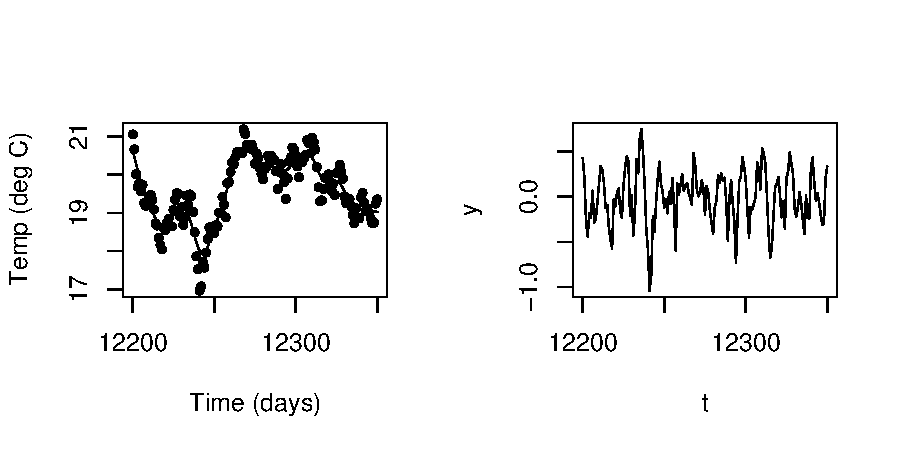
\includegraphics[width=\textwidth]{proto-smoothing03}
\end{center}
\caption{Data and smooth from \code{oo\$plot()} (left) and plot of
\code{oo\$residuals()} (right).}
\label{fig:proto-smooting03}
\end{figure}


Now let us illustrate the creation of a child object and delegation.
We create a new child object of \code{oo} called \code{oo.res}.  We
will override the \code{x} value in its parent by setting \code{x} in
the child to the value of the residuals in the parent.  We will also
override the \code{pch} and \code{ylab} plotting parameters.  We will
return to 1 plot per screen and run \code{plot} using the
\code{oo.res} object as the receiver invoking the \code{smooth} and
\code{plot} methods (which are delegated from the parent \code{oo})
with the data in the child (figure \ref{fig:smoothing04}).

\begin{Schunk}
\begin{Sinput}
> oo.res <- oo$proto(pch = "-", x = oo$residuals()$y, ylab = "Residuals deg K")
> par(mfrow = c(1, 1))
> oo.res$smooth()
> oo.res$plot()
\end{Sinput}
\end{Schunk}

% \begin{figure}[tp]
\begin{figure}[h!]
\begin{center}
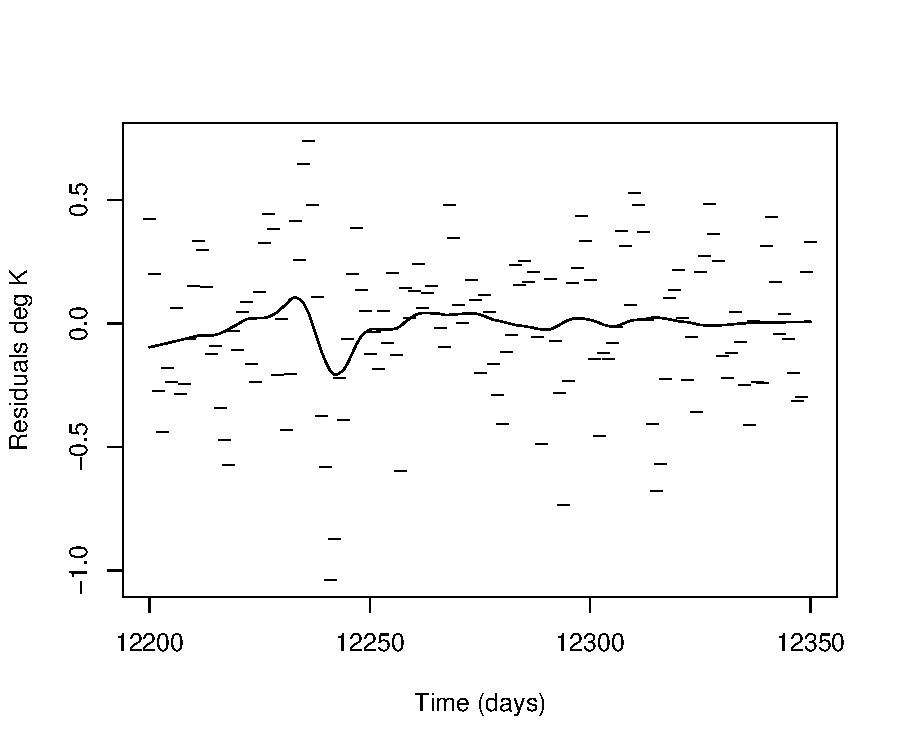
\includegraphics[width=\half]{proto-smoothing04}
\end{center}
\caption{Output of \code{oo.res\$plot()}.
\code{oo.res\$x} contains the residuals from \code{oo}.}
\label{fig:smoothing04}
\end{figure}
Now we make use of delegation to change the parent
and child in a consistent way with respect to certain plot characteristics.
We have been using a numeric time axis.
Let us interpret these numbers as the number of days since the Epoch,
January 1, 1970, and let us also change the plot colors.

\begin{Schunk}
\begin{Sinput}
> oo$tt <- oo$tt + as.Date("1970-01-01")
> oo$xlab <- format(oo.res$tt[1], "%Y")
> oo$col <- c("blue", "red")
\end{Sinput}
\end{Schunk}


We can introduce a new method, \code{splot}, into
the parent \code{oo} and have it automatically
inherited by its children.  In this example
it smooths and then plots and we use it with
both \code{oo} and \code{oo.res} (figure \ref{fig:smoothing06}).


\begin{Schunk}
\begin{Sinput}
> oo$splot <- function(., ...) {
+     .$smooth(...)
+     .$plot()
+ }
> par(mfrow = c(1, 2))
> oo$splot(bass = 2)
> oo.res$splot()
\end{Sinput}
\end{Schunk}


\begin{figure}[tbp]
\begin{center}
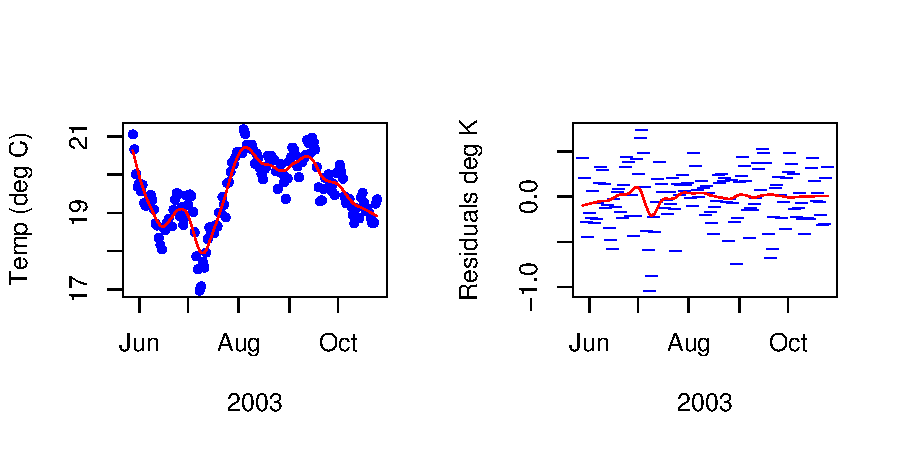
\includegraphics[width=\textwidth]{proto-smoothing06}
\caption{Plotting options and \code{splot} function applied
to both parent (left) and child (right) object}
\label{fig:smoothing06}
\end{center}
\end{figure}

Numerous possibilities exist to make use of the
mechanisms shown, so one may create different child objects, apply
different smoothing parameters, overwrite the smoothing function with
a lowess smoother and finally compare fits and residuals.

Now lets change the data and repeat the analysis.  Rather than
overwrite the data we will preserve it in \code{oo} and create a child
\code{oos} to hold an analysis with sinusoidal data.

\begin{Schunk}
\begin{Sinput}
> oos <- oo$proto(expr = {
+     tt <- seq(0, 4 * pi, length = 1000)
+     x <- sin(tt) + rnorm(tt, 0, 0.2)
+ })
> oos$splot()
\end{Sinput}
\end{Schunk}

Lets perform the residual analysis with \code{oos}.
We will make a deep copy of \code{oo.res}, i.e. duplicate its
contents and not merely delegate it, by copying \code{oo.res}
to a list from which we create the duplicate, or cloned,
\code{proto} object (figure \ref{fig:smoothing10} and \ref{fig:cloning}):

\begin{Schunk}
\begin{Sinput}
> oos.res <- as.proto(oo.res$as.list(), parent = oos)
> oos.res$x <- oos$residuals()$y
> oos.res$splot()
\end{Sinput}
\end{Schunk}


\begin{figure}[tbp]
\begin{center}
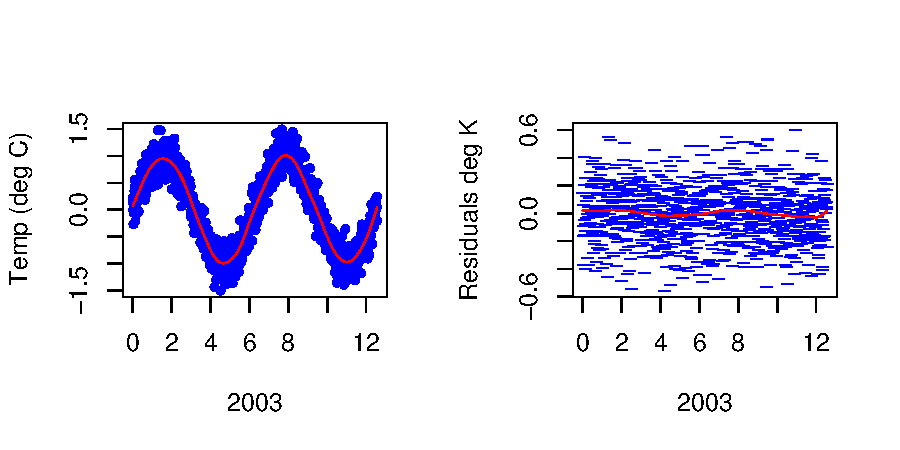
\includegraphics[width=\textwidth]{proto-smoothing10}
\caption{Smoothing of sinusoidal data (left)
and of their residuals (right)}\label{fig:smoothing10}
\end{center}
\end{figure}

\begin{figure}[h!]
\begin{center}
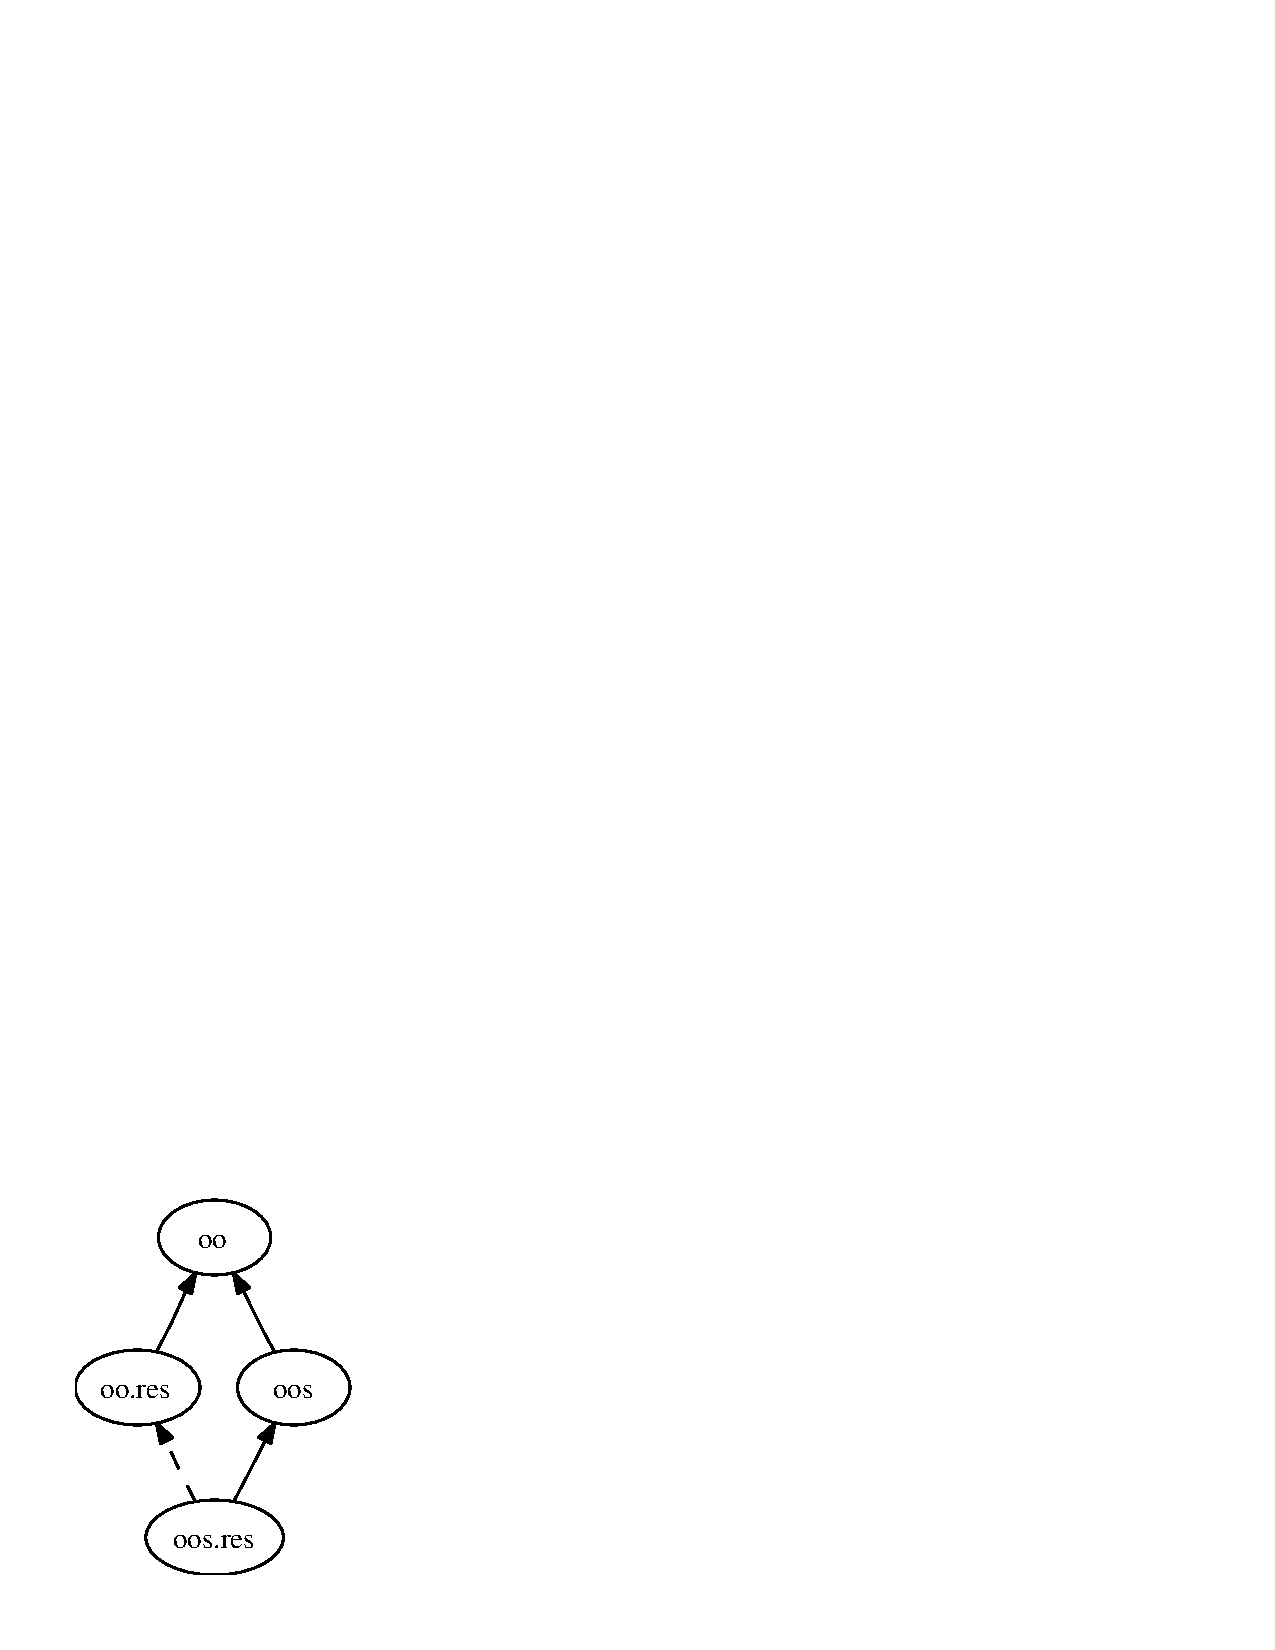
\includegraphics[width=50mm]{cloning3.pdf}
\caption{Cloning (dashed line) and delegation (solid line).  Edges point
from child to parent.}\label{fig:cloning}
\end{center}
\end{figure}

We have delegated variables
and methods and overridden both.
Thus, even with such a simple analysis, object orientation
and delegation came into play.
The reader can plainly see that smoothing and residual
analysis were not crucial to the example and this example
could be replaced with any statistical analysis including
likelihood or other estimation techniques, time series, survival
analysis, stochastic processes and so on.  The key aspect is
just that we are performing one-of analyses and do not want to
set up an elaborate class infrastructure but just want to
directly create objects to organize our calculations while
relying on delegation and dispatch to eliminate redundancy.

\subsection{Correlation, Fisher's Transform and Bootstrapping}
\label{sec:corr}

The common approach to
confidence intervals for the correlation coefficient is to
assume normality of the underlying data and then use Fisher's transform
to transform the correlation coefficient to an approximately normal
random variable.
Fisher showed that with the above normality assumption, transforming
the correlation coefficient using
the hyperbolic arc tangent function
yields a random variable
approximately distributed with an
$\frac{N(p, 1)}{\sqrt(n-3)}$ distribution.  The transformed random
variable can be used to create normal distribution confidence intervals
and the procedure can be back transformed to get confidence intervals
for the original correlation coefficient.

A more recent approach to confidence intervals for the correlation
coefficient is to use bootstrapping.  This does not require the
assumption of normality of the underlying distribution and requires
no special purpose theory devoted solely to the correlation coefficient,

Let us calculate the 95\%
confidence intervals using Fisher's transform
first.  We use \code{GNP} and \code{Unemployed} from the Longley data
set.  First we retrieve the data set and extract the required columns
into \code{x}.  Then we set \code{n} to the number of cases
and \code{pp} to the percentiles
of interest.  Finally we calculate the sample correlation and
create a function to calculate the confidence interval using
Fisher's Transform.  This function not only returns the confidence
interval but also stores it in \code{CI} in the receiver object.

\begin{Schunk}
\begin{Sinput}
> longley.ci <- proto(expr = {
+     data(longley)
+     x <- longley[, c("GNP", "Unemployed")]
+     n <- nrow(x)
+     pp <- c(0.025, 0.975)
+     corx <- cor(x)[1, 2]
+     ci <- function(.) (.$CI <- tanh(atanh(.$corx) + qnorm(.$pp)/sqrt(.$n -
+         3)))
+ })
\end{Sinput}
\end{Schunk}

Now let us repeat this analysis using the bootstrapping approach.  We
derive a new object \code{longley.ci.boot} as child of
\code{longley.ci}, setting the number of replications, \code{N}, and
defining the procedure, \code{ci} which does the actual bootstrap
calculation.

\begin{Schunk}
\begin{Sinput}
> longley.ci.boot <- longley.ci$proto({
+     N <- 1000
+     ci <- function(.) {
+         corx <- function(idx) cor(.$x[idx, ])[1, 2]
+         samp <- replicate(.$N, corx(sample(.$n, replace = TRUE)))
+         (.$CI <- quantile(samp, .$pp))
+     }
+ })
\end{Sinput}
\end{Schunk}

In the example code below the first line runs the Fisher Transform
procedure and the second runs the bootstrap procedure.  Just to check
that we have performed sufficient bootstrap iterations we rerun it in
the third line, creating a delegated object on-the-fly running its
\code{ci} method and then immediately throwing the object away.
The fact that 4,000
replications give roughly the same result as 1,000 replications
satisfies us that we have used a sufficient number of replications.

\begin{Schunk}
\begin{Sinput}
> longley.ci$ci()
\end{Sinput}
\begin{Soutput}
[1] 0.1549766 0.8464304
\end{Soutput}
\begin{Sinput}
> longley.ci.boot$ci()
\end{Sinput}
\begin{Soutput}
     2.5%     97.5%
0.2299395 0.8211854
\end{Soutput}
\begin{Sinput}
> longley.ci.boot$proto(N = 4000)$ci()
\end{Sinput}
\begin{Soutput}
     2.5%     97.5%
0.2480999 0.8259276
\end{Soutput}
\end{Schunk}

We now have the results stored in two objects nicely organized for the
future.  Note, again, that despite the simplicity of the example we
have used the features of object oriented programming, coupling the
data and methods that go together, while relying on delegation and
dispatch to avoid duplication.

\subsection{Dendrograms}
\label{sec:tree}

In \cite{Gentleman2002} there is an \proglang{S4}
example of creating a binary tree
for use as a dendrogram.  Here we directly define a binary tree with no
setup at all.  To keep it short we will create a binary tree of only
two nodes having a root whose left branch points to a leaf.  The leaf
inherits the \code{value} and \code{incr} components from the root.
The attractive feature is that the leaf be defined as a child of the
parent using \code{proto} before the parent is even finished
being defined.  Compared to the cited \proglang{S4} example where it
was necessary to create an extra class to introduce the required level of
indirection there is no need to take any similar action.

\code{tree} is the root node of the tree.  It has four components.  A
method \code{incr} which increments the \code{value} component, a
\code{..Name}, the \code{value} component itself and the left branch
\code{..left}.  \code{..left} is itself a proto object which is a
child of \code{tree}.  The leaf inherits the \code{value} component
from its parent, the root.  As mentioned, at the time we define
\code{..left} we have not even finished defining \code{tree} yet we
are able to implicitly reference the yet to be defined parent.

\begin{Schunk}
\begin{Sinput}
> tree <- proto(expr = {
+     incr <- function(., val) .$value <- .$value + val
+     ..Name <- "root"
+     value <- 3
+     ..left <- proto(expr = {
+         ..Name = "leaf"
+     })
+ })
\end{Sinput}
\end{Schunk}

Although this is a simple structure we could have embedded additional
children into \code{root} and \code{leaf} and so on recursively making
the tree or dendrogram arbitrarily complex.

Let us do some computation with this structure.  We display the
\code{value} fields in the two nodes, increment the value field in the
root and then display the two nodes again to show .that the leaf
changed too.

\begin{Schunk}
\begin{Sinput}
> cat("root:", tree$value, "leaf:", tree$..left$value, "\n")
\end{Sinput}
\begin{Soutput}
root: 3 leaf: 3
\end{Soutput}
\begin{Sinput}
> tree$incr(1)
> cat("root:", tree$value, "leaf:", tree$..left$value, "\n")
\end{Sinput}
\begin{Soutput}
root: 4 leaf: 4
\end{Soutput}
\end{Schunk}

If we increment \code{value} in \code{leaf} directly (see the example
below where we increment it by 10) then it receives its own copy of
\code{value} so from that point on \code{leaf} no longer inherits
\code{value} from \code{root}.  Thus incrementing the root by 5 no
longer increments the \code{value} field in the leaf.

\begin{Schunk}
\begin{Sinput}
> tree$..left$incr(10)
> cat("root:", tree$value, "leaf:", tree$..left$value, "\n")
\end{Sinput}
\begin{Soutput}
root: 4 leaf: 14
\end{Soutput}
\begin{Sinput}
> tree$incr(5)
> cat("root:", tree$value, "leaf:", tree$..left$value, "\n")
\end{Sinput}
\begin{Soutput}
root: 9 leaf: 14
\end{Soutput}
\end{Schunk}

\subsection{From Prototypes to Classes}
\label{sec:increment}

In many cases we will use \pkg{proto} for a design that uses prototypes
during the full development cycle.  In other cases we may use it in an
incremental way starting with prototypes but ultimately transitioning
to classes.
As shown in Section~\ref{sec:traits} the \pkg{proto} package is
powerful enough to handle class-based as well as class-free programming.
Here we illustrate this process of incremental design
starting with
concrete objects and then over time classifing them into classes,
evolving a class-based program.  \pkg{proto} provides a smooth
transition path since it can handle both the class-free and the class-based
phases -- there is no need to switch object systems part way through.
In this example, we define an object which holds a linear equation, \code{eq},
represented as a character string in terms of the unknown variable \code{x}
and a \code{print} and a \code{solve} method.  We execute the
\code{print} method
to solve it.  We also create child object \code{lineq2}
which overrides \code{eq} and execute its \code{print} method.

\begin{Schunk}
\begin{Sinput}
> lineq <- proto(eq = "6*x + 12 - 10*x/4 = 2*x", solve = function(.) {
+     e <- eval(parse(text = paste(sub("=", "-(", .$eq), ")")),
+         list(x = 0+1i))
+     -Re(e)/Im(e)
+ }, print = function(.) cat("Equation:", .$eq, "Solution:", .$solve(),
+     "\n"))
> lineq$print()
\end{Sinput}
\begin{Soutput}
Equation: 6*x + 12 - 10*x/4 = 2*x Solution: -8
\end{Soutput}
\begin{Sinput}
> lineq2 <- lineq$proto(eq = "2*x = 7*x-12+x")
> lineq2$print()
\end{Sinput}
\begin{Soutput}
Equation: 2*x = 7*x-12+x Solution: 2
\end{Soutput}
\end{Schunk}

We could continue with enhancements but at this point we decide that we
have a general case and so wish
to abstract \code{lineq} into a class.  Thus we define a trait,
\code{Lineq}, which is just \code{lineq} minus \code{eq} plus
a constructor \code{new}.  The key difference between \code{new}
and the usual \code{proto} function
is that with \code{new} the initialization of \code{eq} is mandatory.
Having completed this definition
we instantiate an object of
class/trait \code{Lineq} and execute it.

\begin{Schunk}
\begin{Sinput}
> Lineq <- lineq
> rm(eq, envir = Lineq)
> Lineq$new <- function(., eq) proto(., eq = eq)
> lineq3 <- Lineq$new("3*x=6")
> lineq3$print()
\end{Sinput}
\begin{Soutput}
Equation: 3*x=6 Solution: 2
\end{Soutput}
\end{Schunk}

Note how we have transitioned from a prototype style of programming
to a class-based style of programming all the while staying within
the \pkg{proto} framework.

\section{Summary} \label{sec:summary}

\subsection{Benefits}
\label{sec:benefits}

The key benefit of the \pkg{proto} package is to provide
access to a style of programming that has not been conveniently
accessible within \proglang{R} or any other mainstream language today.

\pkg{proto} can be used in two key ways: class-free object oriented programming
and class-based object oriented programming.

A key application for \pkg{proto} in class-free programming is to wrap the code
and data for each run of a particular statistical study into an object for
purposes of organization and reproducibility.  It provides such organization
directly and without the need and overhead of class definitions
yet still provides the
inheritance and dispatch advantages of object oriented programming.
We provide examples of this style of programming in
Section~\ref{sec:smooth}
and
Section~\ref{sec:corr}.
A third example in
Section~\ref{sec:tree} illustrates a beneficial use of \pkg{proto} with
recursive data structures.

Another situation where prototype programming is of interest is in the initial
development stages of a program.  In this case, the design may not be fully
clear so it is more convenient to create concrete objects individually rather
than premature abstractions through classes.  The \code{graph.proto}
function can be used to generate visual representations of the object
tree suggesting classifications of objects so that
as the program evolves the general case becomes clearer and
in a bottom up fashion the objects are incrementally abstracted into
classes.  In this case,
\pkg{proto} provides a smooth transition path since it not only supports
class-free programming but, as explained in the Section~\ref{sec:traits}, is
sufficiently powerful to support class-based programming, as well.


\subsection{Conclusion}
\label{sec:conclusion}

The package \pkg{proto} provides an \proglang{S3} subclass of the
\code{environment} class for constructing and manipulating object
oriented systems without classes.  It can also emulate classes even
though classes are not a primitive structure.  Its key design goals
are to provide as simple and as thin a layer as practically possible
while giving the user convenient access to this alternate object
oriented paradigm.  This paper describes, by example, how prototype
programming can be carried out in \proglang{R} using \pkg{proto} and
illustrates such usage.  Delegation, cloning traits and general
manipulation and incremental development are all reviewed by example.

\section*{Computational details}
\label{sec:compute}

The results in this paper were obtained using \proglang{R} 2.1.0 with
the package \pkg{proto} 0.3--2. \proglang{R} itself and the
\pkg{proto} package are available from CRAN at
\url{http://CRAN.R-project.org/}.  The GraphViz software is available
from \url{http://www.graphviz.org}.

\phantomsection
\addcontentsline{toc}{section}{References}
\bibliography{proto}
%

%\VignetteIndexEntry{proto: An R Package for Prototype Programming}
%\VignetteDepends{}
%\VignetteKeywords{object oriented, prototype programming, S3, R}
%\VignettePackage{proto}


\documentclass[nojss]{jss}
\usepackage{Sweave}
\DeclareGraphicsExtensions{.pdf, .eps, .png}



\newlength{\half}
\setlength{\half}{70mm}

\author{Louis Kates\\GKX Associates Inc. \And
        Thomas Petzoldt\\Technische Universit\"at Dresden}
\Plainauthor{Louis Kates, Thomas Petzoldt}

\title{\pkg{proto}: An \proglang{R} Package for Prototype Programming}
%% \Shorttitle{\pkg{proto}: An \proglang{R} Package for Prototype Programming}

\Plaintitle{proto: An R Package for Prototype Programming}

\Keywords{prototype programming, delegation, inheritance, clone,
  object orientated, \proglang{S3}, \proglang{R}}
\Plainkeywords{object oriented, prototype programming, S3, R}

\Abstract{

  \pkg{proto} is an \proglang{R} package which facilitates a style
  of programming known as prototype
  programming.  Prototype programming is a type of object
  oriented programming in which there are no classes.
  \pkg{proto} is simple yet retains the object oriented features of
  delegation (the prototype counterpart to inheritance)
  and object oriented  dispatch.  \code{proto} can be used
  to organize the concrete data and procedures in statistical studies
  and other applications
  without the necessity of defining classes while still providing convenient
  access to an object oriented style of programming.  Furthermore, it
  can be used in a class-based style as well so that incremental design can
  begin with defining the concrete objects and later transition to abstract
  classes, once the general case is understood, without having to change to
  object-oriented frameworks.
  The key goals of the package are to integrate into \proglang{R}
  while providing nothing more than a thin layer on top of it.
}

\hyphenation{ma-ni-pu-lating}

\begin{document}
\Sconcordance{concordance:proto.tex:proto.Rnw:%
1 1362 1}





\section{Introduction} \label{sec:intro}

\subsection[Object Oriented Programming in R]{Object Oriented Programming in \proglang{R}}
\label{sec:oo}

The \proglang{R} system for statistical computing
\citep[\url{http://www.R-project.org/}]{Rcore2005} ships with two
systems for object oriented programming referred to as \proglang{S3}
and \proglang{S4}.  With the increased interest in object oriented
programming within \proglang{R} over the last years additional object
oriented programming packages emerged.  These include the \pkg{R.oo}
package \citep{Bengtsson2003} and the \pkg{OOP} package
\citep[\url{http://www.omegahat.net/OOP/}]{Rnews:Chambers+Lang:2001a}.
All these packages have the common thread that they use
classes as the basis of inheritance.  When a message is sent to an
object the class of the object is examined and that class determines the
specific function to be executed. In prototype programming there
are no classes making it simple yet it retains much of the power of
class-based programming.  In the fact, \pkg{proto} is so simple that
there is only one significant new routine name, \code{proto}.  The
other routines are just the expected support routines such as
\code{as.proto} to coerce objects to proto objects, \code{\$} to
access and set proto object components and \code{is.proto} to check
whether an object is a proto object.  In addition, \code{graph.proto}
will generate a graphical ancestor tree showing the parent-child
relationships among generated \code{proto} objects.

The aim of the package is to provide a lightweight layer for prototype
programming in \proglang{R} written only in \proglang{R} leveraging the
existing facilities of the language rather than adding its own.

\subsection{History}
\label{sec:history}

The concept of
prototype programming
\citep{Lieberman1986, Taivalsaari1996a, Noble1999}
has developed over a number of years with the \proglang{Self}
language \citep{Agesen1992}
being the key evolved programming language to demonstrate
the concept.  In statistics, the \proglang{Lisp}-based
\proglang{LispStat} programming language \citep{Tierney1990} was
the first and possibly only statistical system to feature prototype
programming.

Despite having been developed over 20 years ago, and some attempts to
enter the mainstream (e.g.  \proglang{Newtonscript}
on the Newton computer, which
is no longer available, and \proglang{Javascript} where
it is available but whose
domain of application largely precluses use of prototype programming)
prototype programming is not well known due to lack of language
support in popular programming languages such as \proglang{C} and
\proglang{Java}.  It tends
to be the domain of research languages or \proglang{Lisp}.

Thus the
the availability of a popular language,
\proglang{R} \footnote{Some indications of the popularity of R are
the high volume mailing lists, international development team, the
existence of over 500 addon packages, conferences and numerous books
and papers devoted to R.},
that finally does provide the key infrastructure
is an important development.

This work grew out of the need to organize multiple scenarios of model
simulations in ecological modelling \citep{Rnews:Petzoldt:2003} and
was subsequently generalized to the present package.  A number of
iterations of the code, some motivated by the ever increasing feature
set in \proglang{R}, resulted in a series of utilities and ultimately
successive versions of an \proglang{R} package developed over the last
year.  An initial version used \proglang{R} lists as the basis of the
package.  Subsequently the package was changed to use \proglang{R}
environments.  The first version to use environments stored the
receiver object variable in a proxy parent environment which was
created on-the-fly at each method call.  The present version of
the \pkg{proto} package passes the receiver object through the argument list,
while hiding this from the caller.  It defines the \code{proto} class
as a subclass of the \code{environment} class so that
functionality built into \proglang{R} for the environment class is
automatically inherited by the \code{proto} class.

\subsection{Overview}
\label{sec:overview}

It is assumed that the reader has some general
familiarity with object oriented programming concepts and with
\proglang{R}.

The paper will proceed primarily by example focusing on illustrating
the package \code{proto} through such demonstration.  The remainder of
the paper is organized as follows: Section~\ref{sec:proto-class}
explains how \code{"proto"} objects are created and illustrates the
corresponding methods for setting and getting components.  It further
discusses how object oriented delegation (the prototype programming
analogue of inheritance) is handled and finally discusses the
internals of the package.  This section uses small examples chosen for
their simplicity in illustrating the concepts.  In
Section~\ref{sec:examples} we provide additional examples of prototype
programming in action.  Four examples are shown.  The first involves
smoothing of data.  Secondly we demonstrate the calculation of
correlation confidence intervals using classical (Fisher Transform)
and modern (bootstrapping) methods.  Thirdly we demonstrate the
development of a binary tree as would be required for a dendrogram.
Fourthly, we use the solution of linear equations to illustrate
program evolution from object-based to class-based, all
within the \pkg{proto} framework.
Section~\ref{sec:summary} gives a few summarizing remarks.  Finally,
an appendix provides a reference card that summarizes the
functionality contained in \pkg{proto} in terms of its constituent
commands.

%% \pagebreak[4]

\section[The class "proto" and its methods]{The class \code{"proto"} and its methods}
\label{sec:proto-class}

\subsection[Creation of "proto" objects]{Creation of \code{"proto"} objects}
\label{sec:proto}

In this section we shall show, by example, the creation of two
prototype objects and related operations.  The simple idea is that
each \code{"proto"} object is a set of components: functions (methods)
and variables, which are tightly related in some way.

A prototype object is an environment holding the variables and
methods of the object. \footnote{In particular this implies that
\code{"proto"} objects have single inheritance, follow ordinary
environment scoping rules and have mutable state as environments
do.}

A prototype object is created using the constructor function
\code{proto} (see Appendix~\ref{sec:ref} at the end of this paper or
\pkg{proto} package help for complete syntax of commands).

\begin{Scode}
addProto <- proto( x = rnorm(5), add = function(.) sum(.$x) )
\end{Scode}

In this simple example, the \code{proto} function defines two
components: a variable \code{x} and a method \code{add}.  The variable
\code{x} is a vector of 5 numbers and the method sums those numbers.
The \code{proto} object \code{addProto} contains the variable and the
method.  Thus the \code{addProto} \code{proto} object can be used to compute
the sum of the values stored in it.
As shown with the \code{add} method in this example, formal argument
lists of methods must always have a first argument of dot
(i.e. \code{.})  which signifies the object on which the method is
operating.  The dot refers to the current object in the same way that
a dot refers to the current directory in UNIX.  Within the method one
must refer to other variables and methods in the object by prefacing
each with \code{.\$}.  For example, in the above we write
\code{sum(.\$x)}.  Finally, note that the data and the method are very
closely related.  Such close coupling is important in order to create
an easily maintained system.

To illustrate the usage of \code{proto}, we first load the package and
set the random seed to make the examples in this paper exactly
reproducible.

\begin{Schunk}
\begin{Sinput}
> library(proto)
> set.seed(123)
\end{Sinput}
\end{Schunk}

Then, we create the \code{proto} object from above
and call its \code{add} method.
\begin{Schunk}
\begin{Sinput}
> addProto <- proto(x = rnorm(5), add = function(.) sum(.$x))
> addProto$add()
\end{Sinput}
\begin{Soutput}
[1] 0.9678513
\end{Soutput}
\end{Schunk}
We also create another object, \code{addProto2}
with a different \code{x} vector and
invoke its \code{add} method too.
\begin{Schunk}
\begin{Sinput}
> addProto2 <- addProto$proto(x = 1:5)
> addProto2$add()
\end{Sinput}
\begin{Soutput}
[1] 15
\end{Soutput}
\end{Schunk}
In the examples above, we created a prototype object \code{addProto}
and then called its \code{add} method as just explained.
The notation \code{addProto\$add}
tells the system to look for the \code{add} method
in the \code{addProto} object.  In the expression \code{addProto\$add},
the \code{proto} object to the left
of the dollar sign, \code{addProto} here, is referred to as the
\emph{receiver} object.  This expression
also has a second purpose which is to
pass the receiver object implicitly as the first argument of \code{add}.
Note that we called \code{add} as if it had zero arguments but, in fact,
it has one argument because the receiver is automatically and implicitly
supplied as the first argument.  In general,
the notation \code{object\$method(arguments)} is
used to invoke the indicated method of the receiver object using the
object as the implicit first argument along with the indicated
arguments as the subsequent arguments.
As with the \code{addProto} example, the receiver
object not only determines where to find the
method but also is implicitly passed to the method through
the first argument.  The motivation for this notation
is to relieve the user of
specifying the receiver object twice:
once to locate the method in the object and a second
time to pass the object itself to the method.
The \code{\$} is overloaded by the \code{proto}
class to automatically do both with one reference to the receiver object.
Even though, as with the \code{addProto} example, the first
argument is not listed in the call
it still must be listed among the formal arguments
in the definition of the method.  It
is conventional to use
a dot \code{.} as the first formal argument in the method/function
definition.  That is, we call \code{add} using \code{addProto\$add()}
displaying zero arguments
but we define \code{add} in \code{addProto} displaying
one argument \code{add <- function(.)}, the dot.

In this example,
we also created a second object, \code{addProto2},
which has the first object, \code{addProto} as its parent.
Any reference to a
component in the second object that is unsuccessful will cause
search to continue in the parent.  Thus the call \code{addProto2\$add()}
looks for \code{add} in \code{addProto2} and not finding it there
searches its parent, \code{addProto}, where it is, indeed, found.
\code{add} is invoked with the receiver object, \code{addProto2}, as
the value of dot.
The call \code{addProto2\$add()} actually causes the \code{add}
in \code{addProto} to run but it still uses the \code{x} from
\code{addProto2} since dot (\code{.}) is \code{addProto2} here
and \code{add} references \code{.\$x}.
Note that the reference to \code{.\$x} in the
\code{add} found in \code{addProto}
does not refer to the \code{x} in \code{addProto} itself.
The \code{x} in \code{addProto2} has overridden the \code{x} in its parent.
This point is important so the reader should take care to absorb this
point.

This simple example already shows the key elements of the system
and how \emph{delegation} (the prototype programming term for inheritance)
works without classes.

We can add new components or replace components in an object and
invoke various methods like this:
\begin{Schunk}
\begin{Sinput}
> addProto2$y <- seq(2, 10, 2)
> addProto2$x <- 1:10
> addProto2$add3 <- function(., z) sum(.$x) + sum(.$y) + sum(z)
> addProto2$add()
\end{Sinput}
\begin{Soutput}
[1] 55
\end{Soutput}
\begin{Sinput}
> addProto2$add3(c(2, 3, 5))
\end{Sinput}
\begin{Soutput}
[1] 95
\end{Soutput}
\begin{Sinput}
> addProto2$y
\end{Sinput}
\begin{Soutput}
[1]  2  4  6  8 10
\end{Soutput}
\end{Schunk}

In this example, we insert variable \code{y} into the object \code{addProto2}
with a value of \code{seq(2,10,2)},
reset variable \code{x} to a new value and insert a new method,
\code{add3}. Then we invoke
our two methods and display \code{y}.  Again, note that in the case of
\code{protoAdd2\$add} the \code{add} method is not present in
\code{protoAdd2} and so search continues to the parent \code{addProto}
where it is found.

\subsection{Internals}
\label{sec:internals}

So far, we have used simple examples to illustrate the basic manipulation
of objects: construction, getting and setting components and method
invocation.  We now discuss the internals of the package and how it relates
to \proglang{R} constructs.
\code{proto} is actually an \proglang{S3} class which is a subclass
of the \code{environment} class.  Every \code{proto} object is an
environment and its class is \code{c("proto", "environment")}.  The \code{\$}
accessor is similar to the same accessor in environments except it will
use the \proglang{R} \code{get} function to
search up parent links if it cannot otherwise find the object (unlike
environments).  When accessing a method, \code{\$}
automatically supplies the
first argument to the method
unless the object is \code{.that} or \code{.super}.  \code{.that}
is a special variable which \code{proto} adds to every \code{proto} object
denoting the object itself.  \code{.super} is also added to every
proto object and is the parent of \code{.that}.  \code{.that}
and \code{.super} are normally used
within methods of an object to refer to other components of the same
or parent object, respectively,
as opposed to the receiver (\code{.}).  For example,
suppose we want \code{add} in \code{addProto2} to add the elements
of \code{x} together and the elements of
\code{y} together and then add these two sums.  We could redefine add like this:

\begin{Schunk}
\begin{Sinput}
> addProto2$add <- function(.) .super$add(.) + sum(.$y)
\end{Sinput}
\end{Schunk}

making use of the \code{add} already defined in the parent.
One exception should be noted here.  When one uses \code{.super},
as above, or \code{.that} to specify a method then the receiver
object must be explicitly specified
in argument one (since in those cases the receiver
is possibly different than
\code{.super} or \code{.that} so the system cannot automatically supply it
to the call.)

Setting a value is similar to the corresponding operation for
environments except that any function, i.e method, which is
inserted has its environment set to the environment of the object
into which it is being inserted.  This is necessary so that such
methods can reference \code{.that} and \code{.super} using
lexical scoping.

In closing this section a few points should be re-emphasized and
expanded upon.  A
\code{proto} object is an environment whose parent object is the
parent environment of the \code{proto} object.  The methods in the \code{proto}
objects are ordinary functions that have the containing object as their
environment.

The \proglang{R} \code{with} function can be used with environments and
therefore can be used with \code{proto} objects since \code{proto}
objects are environments too.  Thus \code{with(addProto, x)} refers
to the variable \code{x} in \code{proto} object \code{addProto}
and \code{with(addProto, add)} refers to the method \code{add}
in the same way.  \code{with(addProto, add)(addProto)} can be used
to call \code{add}.  These constructs all follow from their corresponding
use in environments from which they are inherited.

Because the \code{with} expressions are somewhat verbose, two common
cases can be shortened using the \code{\$} operator.  \code{addProto\$x}
can be used to refer to variable \code{x} in \code{proto} object
\code{addProto} and has the same meaning as \code{with(addProto, x)}.
In particular like \code{with} but
unlike the the behavior of the \code{\$} operator on
environments, when used with \code{proto} objects, \code{\$} will
search not only the object itself but also its ancestors.
Similarly \code{addProto\$add()} can be used to call
method \code{add} in \code{addProto} also searching through ancestors
if not found in \code{addProto}.  Note that \code{addProto\$add}
returns an object of class

\code{c("instantiatedProtoMethod", "function")}
which is derived from \code{add} such that the first argument,
the \code{proto} object,
is already inserted.  Note that there is a \code{print} method for
class \code{"instantiatedProtoMethod"} so printing such objects will
display the underlying function but returning such objects
is not the same as returning the function without slot one inserted.
Thus, if one wants exactly the original \code{add}
as a value one should use \code{with(addProto, add)} or
\code{addProto\$with(add)}.

Within a method, if a variable is referred to without
qualification simply as \code{x}, say, then  its meaning  is
unchanged from how it is otherwise used in \proglang{R} and
follows the same scope rules as any variable to resolve its name.  If it is
desired that the variable have object scope, i.e. looked up
in the receiver object and its ancestors, then \code{.\$x}
or similar \code{with} notation, i.e. \code{with(., x)}, should be used.
Similarly \code{.\$f(x)} calls
method \code{f} automatically inserting the receiver object
into argument one and using \code{x} for argument two.  It
looks for \code{f} first in the receiver object and then its
ancestors.

\subsection{Traits}
\label{sec:traits}

Let us look at the definition of a child object once again.
In the code below,
\code{addProto} is the previously defined parent object
and the expression \code{addProto\$proto(x = 1:5)} defines
a child object of \code{addProto} and assigns it to variable
\code{addProto2a}.

\begin{Schunk}
\begin{Sinput}
> addProto2a <- addProto$proto(x = 1:5)
> addProto2a$add()
\end{Sinput}
\begin{Soutput}
[1] 15
\end{Soutput}
\end{Schunk}

That is, \code{proto} can be used to create a new child of
an existing object by writing the
parent object on the left of the \code{\$} and
\code{proto} on its right.  Any contents to
be added to the new child are listed in arguments of \code{proto}
as shown.

For example, first let us create a class-like structure.  In the
following \code{Add} is an object that behaves very much like a class
with an \code{add} method and a method \code{new} which constructs
new objects.  In the line creating object \code{add1} the expression
\code{Add\$new(x = 1:5)} invokes the \code{new} constructor of the
receiver object \code{Add}. The method \code{new} has an argument of
\code{x = 1:5} which defines an \code{x} variable in the \code{add1}
object being instantiated. We similarly create another object
\code{add2}.

\begin{Schunk}
\begin{Sinput}
> Add <- proto(add = function(.) sum(.$x), new = function(., x) .$proto(x = x))
> add1 <- Add$new(x = 1:5)
> add1$add()
\end{Sinput}
\begin{Soutput}
[1] 15
\end{Soutput}
\begin{Sinput}
> add2 <- Add$new(x = 1:10)
> add2$add()
\end{Sinput}
\begin{Soutput}
[1] 55
\end{Soutput}
\end{Schunk}

An object which contains only methods and variables that are
intended to be shared by all its children (as opposed to an
object whose purpose is to have its own methods and variables)
is known as a \emph{trait} \citep{Agesen1992}.  It
is similar to a class in class-based
object oriented programming.
Note that the objects \code{add1} and \code{add2} have the trait
\code{Add} as their parent.  We could implement subclass-like and
superclass-like objects by simply defining similar trait objects to
be the parent or child of \code{Add}.  For example, suppose we
want a class which calculates the sum of the logarithms of the data.  We
could define:

\begin{Schunk}
\begin{Sinput}
> Logadd <- Add$proto(logadd = function(.) log(.$add()))
> logadd1 <- Logadd$new(1:5)
> logadd1$logadd()
\end{Sinput}
\begin{Soutput}
[1] 2.70805
\end{Soutput}
\end{Schunk}

Here the capitalized objects are traits.
\code{Logadd} is a trait.  It is a child of \code{Add}
which is also a trait.  \code{logadd1} is an ordinary object,
not a trait.
One possible design is to create a tree of traits and other objects
in which the leaves are ordinary objects and the remaining nodes
are traits.  This would closely correspond to class-based
object oriented programming.

Note that the delegation of methods from
one trait to another as in
\code{new} which is inherited by \code{Logadd} from \code{Add}
is nothing more than the same mechanism by which traits delegate
methods to
objects since, of course, traits are just objects no different
from any other object other than by the conventions we impose on them.
This unification of subclassing and instantiation beautifully
shows the simplification that prototype programming represents.

\subsection{Utilities}
\label{sec:utilities}
The fact that method calls automatically insert the first argument
can be used to good effect in leveraging existing \proglang{R}
functions while allowing an object-oriented syntax.

For example, \code{ls()} can be used to list the components of
\code{proto} objects:

\begin{Schunk}
\begin{Sinput}
> addProto$ls()
\end{Sinput}
\begin{Soutput}
[1] "add" "x"
\end{Soutput}
\end{Schunk}

Functions like:

\begin{Schunk}
\begin{Sinput}
> addProto$str()
> addProto$print()
> addProto$as.list()
> addProto2a$parent.env()
\end{Sinput}
\end{Schunk}

show additional information about the elements.  \code{eapply}
can be used to explore more properties such as the
the length of each component of an object:

\begin{Schunk}
\begin{Sinput}
> addProto$eapply(length)
\end{Sinput}
\end{Schunk}

Another example of some interest in any object oriented system
which allows multiple references to one single object is that
object identity
can be tested using the respective base function:

\begin{Schunk}
\begin{Sinput}
> addProto$identical(addProto2)
\end{Sinput}
\begin{Soutput}
[1] FALSE
\end{Soutput}
\end{Schunk}

\code{proto} does contain a special purpose \code{str.proto} function
but in the main it
is important to notice here, that
\code{proto} has no code that is specific to \code{ls} or
any of the other ordinary \proglang{R}
functions listed.  We are simply making use of the
fact that \code{obj\$fun(...)} is transformed into \code{get("fun",
obj)(obj, ...)} by the proto \code{\$} operator.  For example, in the
case of \code{addProto\$ls()} the system looks for \code{ls} in object
\code{addProto}.  It cannot find it there so it looks to its parent,
which is the global environment.  It does not find it there so it
searches the remainder of the search path, i.e. the path shown by
running the \proglang{R} command \code{search()}, and finally finds it
in the base package, invoking it with an argument of \code{addProto}.
Since all \code{proto} objects are also environments
\code{ls(addProto)} interprets \code{addProto} as an environment and
runs the \code{ls} command with it.  In the \code{ls} example there
were no arguments other than \code{addProto}, and even that one was
implicit, but if there were
additional arguments then they would be passed as shown in the
\code{eapply} and \code{identical} examples above.

\subsection{Plotting}
\label{sec:plot}

The \code{graph.proto} function can be used to create
graphs that can be rendered by the \code{Rgraphviz} package
creating visual representations of ancestor trees (figure
\ref{fig:proto-dot}).
That package provides an interface to the
\proglang{GraphViz} \code{dot} program \citep{Ganser+North:1999}.

\code{graph.proto} takes three arguments, all of which are
usually omitted.  The first argument is a \code{proto} object
(or an environment) out of which all contained \code{proto} objects
and their parents (but not higher order ancestors) are graphed.
If it is omitted, the current environment is assumed.
The second argument is a graph (in the sense of the \code{graph}
package) to which the nodes and edges are added.  If it is omitted
an empty graph is assumed.  The last argument is a logical variable
that specifies the orientation of arrows.  If omitted arrows are
drawn from children to their parents.


\begin{Schunk}
\begin{Sinput}
> library(Rgraphviz)
> g <- graph.proto()
> plot(g)
\end{Sinput}
\end{Schunk}


\begin{figure}[htbp]
\begin{center}
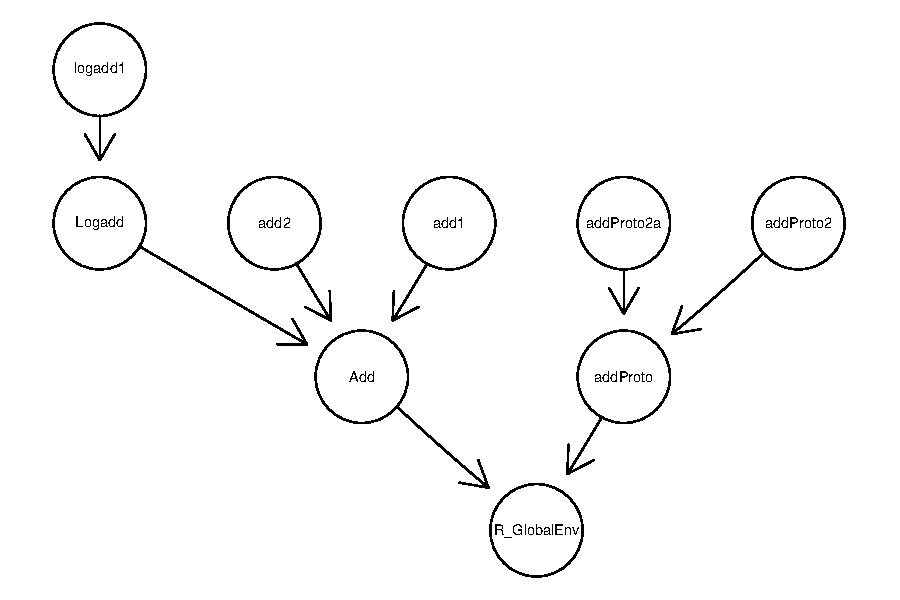
\includegraphics{proto-dot}
\caption{\label{fig:proto-dot} Ancestor tree generated using graph.proto. Edges
point from child to parent.}
\end{center}
\end{figure}

\pagebreak[4]

\section{Examples}
\label{sec:examples}

\subsection{Smoothing}
\label{sec:smooth}

In the following we create a \code{proto} object named \code{oo}
containing a vector of data \code{x} (generated from a simulated
autoregressive model) and time points
\code{tt}, an intermediate result
\code{x.smooth}, some plotting parameters \code{xlab}, \code{ylab},
\code{pch}, \code{col} and three methods \code{smooth}, \code{plot}
and \code{residuals} which smooth the data, plot the data and
calculate residuals, respectively.  We also define \code{..x.smooth}
which holds intermediate results.  Names beginning with two dots
prevent them from being delegated to children.  If we override
\code{x} in a child we would not want an out-of-sync \code{x.smooth}.
Note that the components of an object can be specified using a code
block in place of the argument notation we used previously in the
\code{proto} command.

\begin{Schunk}
\begin{Sinput}
> oo <- proto(expr = {
+     x <- rnorm(251, 0, 0.15)
+     x <- filter(x, c(1.2, -0.05, -0.18), method = "recursive")
+     x <- unclass(x[-seq(100)]) * 2 + 20
+     tt <- seq(12200, length = length(x))
+     ..x.smooth <- NA
+     xlab <- "Time (days)"
+     ylab <- "Temp (deg C)"
+     pch <- "."
+     col <- rep("black", 2)
+     smooth <- function(., ...) {
+         .$..x.smooth <- supsmu(.$tt, .$x, ...)$y
+     }
+     plot <- function(.) with(., {
+         graphics::plot(tt, x, pch = pch, xlab = xlab, ylab = ylab,
+             col = col[1])
+         if (!is.na(..x.smooth[1]))
+             lines(tt, ..x.smooth, col = col[2])
+     })
+     residuals <- function(.) with(., {
+         data.frame(t = tt, y = x - ..x.smooth)
+     })
+ })
\end{Sinput}
\end{Schunk}

Having defined our \code{proto} object we can inspect it, as shown
below, using
\code{print} which is automatically invoked if the
name of the object, \code{oo}, is entered on a line by itself.
In this case, there is no proto print method so we inherit the
environment print method which displays the environment hash code.
Although it produces too much output to show here,
we could have displayed a
list of the entire contents of the object \code{oo}
via \code{oo\$as.list(all.names = TRUE)}.
We can get a list of the names of the
components of the object using \code{oo\$ls(all.names = TRUE)} and will look
at the contents of one component, \code{oo\$pch}.

\begin{Schunk}
\begin{Sinput}
> oo
\end{Sinput}
\begin{Soutput}
<environment: 0x01fbd8c8>
attr(,"class")
[1] "proto"       "environment"
\end{Soutput}
\begin{Sinput}
> oo$ls(all.names = TRUE)
\end{Sinput}
\begin{Soutput}
 [1] "..x.smooth" ".super"     ".that"      "col"        "pch"
 [6] "plot"       "residuals"  "smooth"     "tt"         "x"
[11] "xlab"       "ylab"
\end{Soutput}
\begin{Sinput}
> oo$pch
\end{Sinput}
\begin{Soutput}
[1] "."
\end{Soutput}
\end{Schunk}

Let us illustrate a variety of manipulations.  We will set up the
output to plot 2 plots per screen using \code{mfrow}.  We change the
plotting symbol, smooth the data, invoke the \code{plot} method to
display a plot of the data and the smooth and then plot the residuals
in the second plot (figure \ref{fig:proto-smooting03}).


\begin{Schunk}
\begin{Sinput}
> par(mfrow = c(1, 2))
> oo$pch <- 20
> oo$smooth()
> oo$plot()
> plot(oo$residuals(), type = "l")
\end{Sinput}
\end{Schunk}


\begin{figure}[h!]
\begin{center}
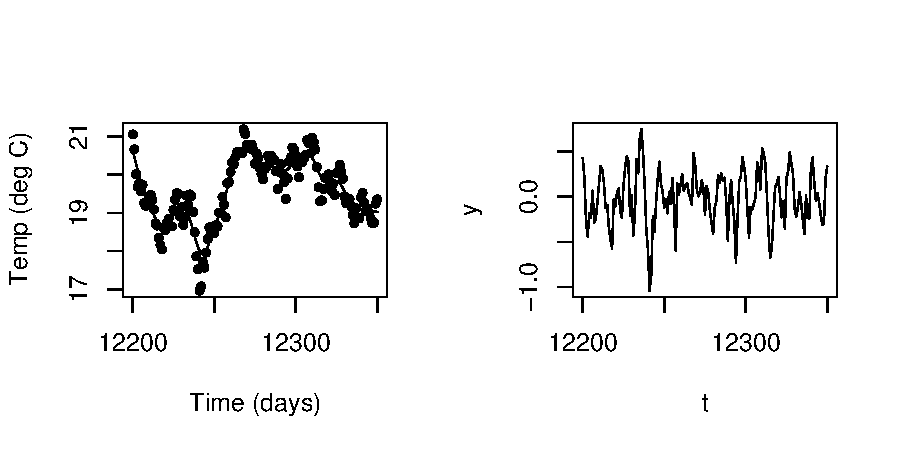
\includegraphics[width=\textwidth]{proto-smoothing03}
\end{center}
\caption{Data and smooth from \code{oo\$plot()} (left) and plot of
\code{oo\$residuals()} (right).}
\label{fig:proto-smooting03}
\end{figure}


Now let us illustrate the creation of a child object and delegation.
We create a new child object of \code{oo} called \code{oo.res}.  We
will override the \code{x} value in its parent by setting \code{x} in
the child to the value of the residuals in the parent.  We will also
override the \code{pch} and \code{ylab} plotting parameters.  We will
return to 1 plot per screen and run \code{plot} using the
\code{oo.res} object as the receiver invoking the \code{smooth} and
\code{plot} methods (which are delegated from the parent \code{oo})
with the data in the child (figure \ref{fig:smoothing04}).

\begin{Schunk}
\begin{Sinput}
> oo.res <- oo$proto(pch = "-", x = oo$residuals()$y, ylab = "Residuals deg K")
> par(mfrow = c(1, 1))
> oo.res$smooth()
> oo.res$plot()
\end{Sinput}
\end{Schunk}

% \begin{figure}[tp]
\begin{figure}[h!]
\begin{center}
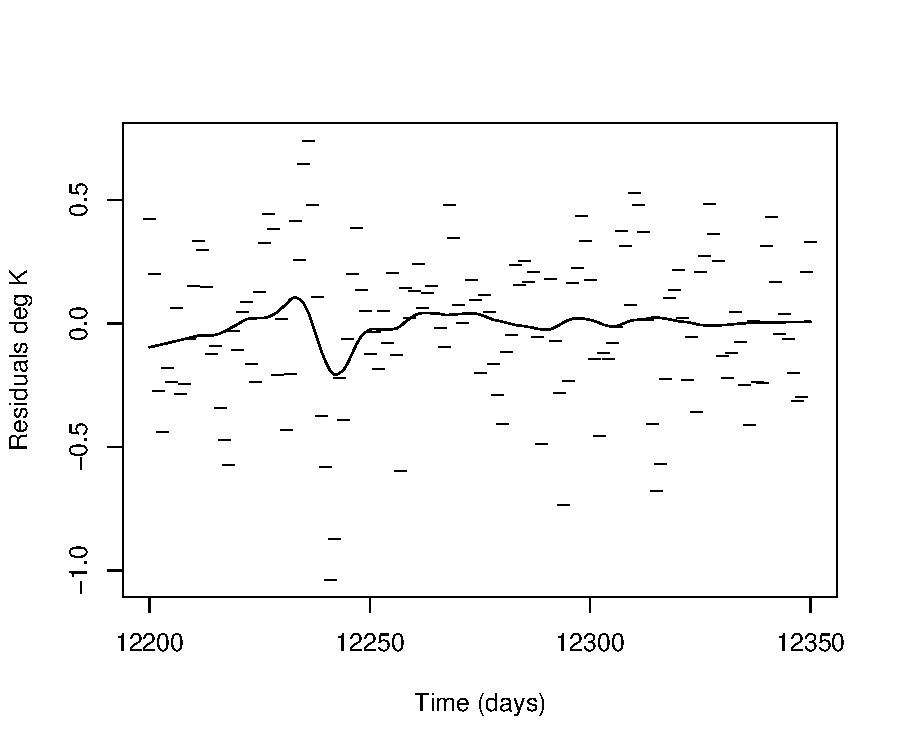
\includegraphics[width=\half]{proto-smoothing04}
\end{center}
\caption{Output of \code{oo.res\$plot()}.
\code{oo.res\$x} contains the residuals from \code{oo}.}
\label{fig:smoothing04}
\end{figure}
Now we make use of delegation to change the parent
and child in a consistent way with respect to certain plot characteristics.
We have been using a numeric time axis.
Let us interpret these numbers as the number of days since the Epoch,
January 1, 1970, and let us also change the plot colors.

\begin{Schunk}
\begin{Sinput}
> oo$tt <- oo$tt + as.Date("1970-01-01")
> oo$xlab <- format(oo.res$tt[1], "%Y")
> oo$col <- c("blue", "red")
\end{Sinput}
\end{Schunk}


We can introduce a new method, \code{splot}, into
the parent \code{oo} and have it automatically
inherited by its children.  In this example
it smooths and then plots and we use it with
both \code{oo} and \code{oo.res} (figure \ref{fig:smoothing06}).


\begin{Schunk}
\begin{Sinput}
> oo$splot <- function(., ...) {
+     .$smooth(...)
+     .$plot()
+ }
> par(mfrow = c(1, 2))
> oo$splot(bass = 2)
> oo.res$splot()
\end{Sinput}
\end{Schunk}


\begin{figure}[tbp]
\begin{center}
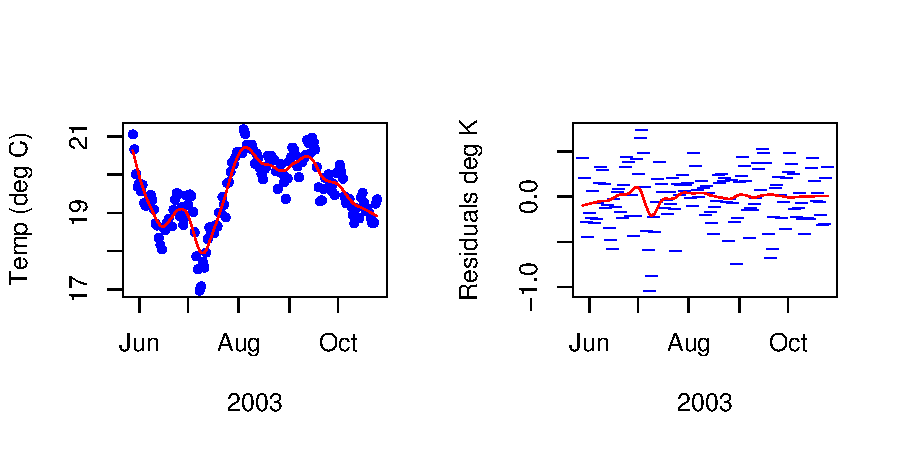
\includegraphics[width=\textwidth]{proto-smoothing06}
\caption{Plotting options and \code{splot} function applied
to both parent (left) and child (right) object}
\label{fig:smoothing06}
\end{center}
\end{figure}

Numerous possibilities exist to make use of the
mechanisms shown, so one may create different child objects, apply
different smoothing parameters, overwrite the smoothing function with
a lowess smoother and finally compare fits and residuals.

Now lets change the data and repeat the analysis.  Rather than
overwrite the data we will preserve it in \code{oo} and create a child
\code{oos} to hold an analysis with sinusoidal data.

\begin{Schunk}
\begin{Sinput}
> oos <- oo$proto(expr = {
+     tt <- seq(0, 4 * pi, length = 1000)
+     x <- sin(tt) + rnorm(tt, 0, 0.2)
+ })
> oos$splot()
\end{Sinput}
\end{Schunk}

Lets perform the residual analysis with \code{oos}.
We will make a deep copy of \code{oo.res}, i.e. duplicate its
contents and not merely delegate it, by copying \code{oo.res}
to a list from which we create the duplicate, or cloned,
\code{proto} object (figure \ref{fig:smoothing10} and \ref{fig:cloning}):

\begin{Schunk}
\begin{Sinput}
> oos.res <- as.proto(oo.res$as.list(), parent = oos)
> oos.res$x <- oos$residuals()$y
> oos.res$splot()
\end{Sinput}
\end{Schunk}


\begin{figure}[tbp]
\begin{center}
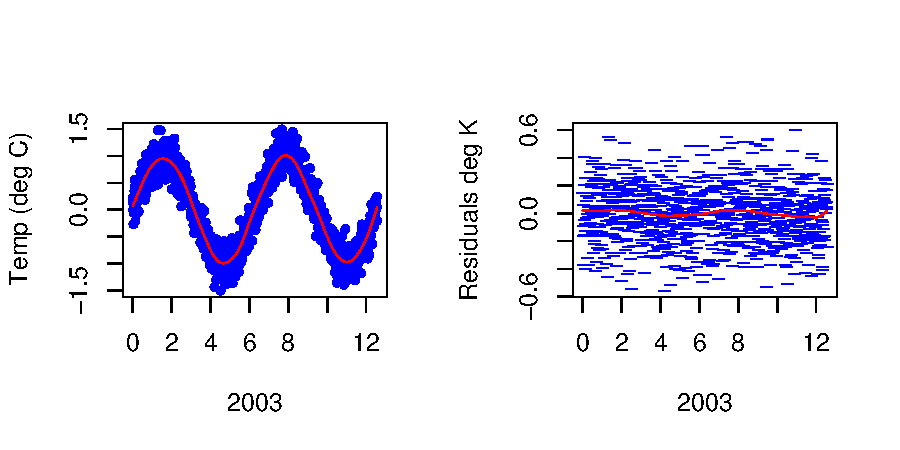
\includegraphics[width=\textwidth]{proto-smoothing10}
\caption{Smoothing of sinusoidal data (left)
and of their residuals (right)}\label{fig:smoothing10}
\end{center}
\end{figure}

\begin{figure}[h!]
\begin{center}
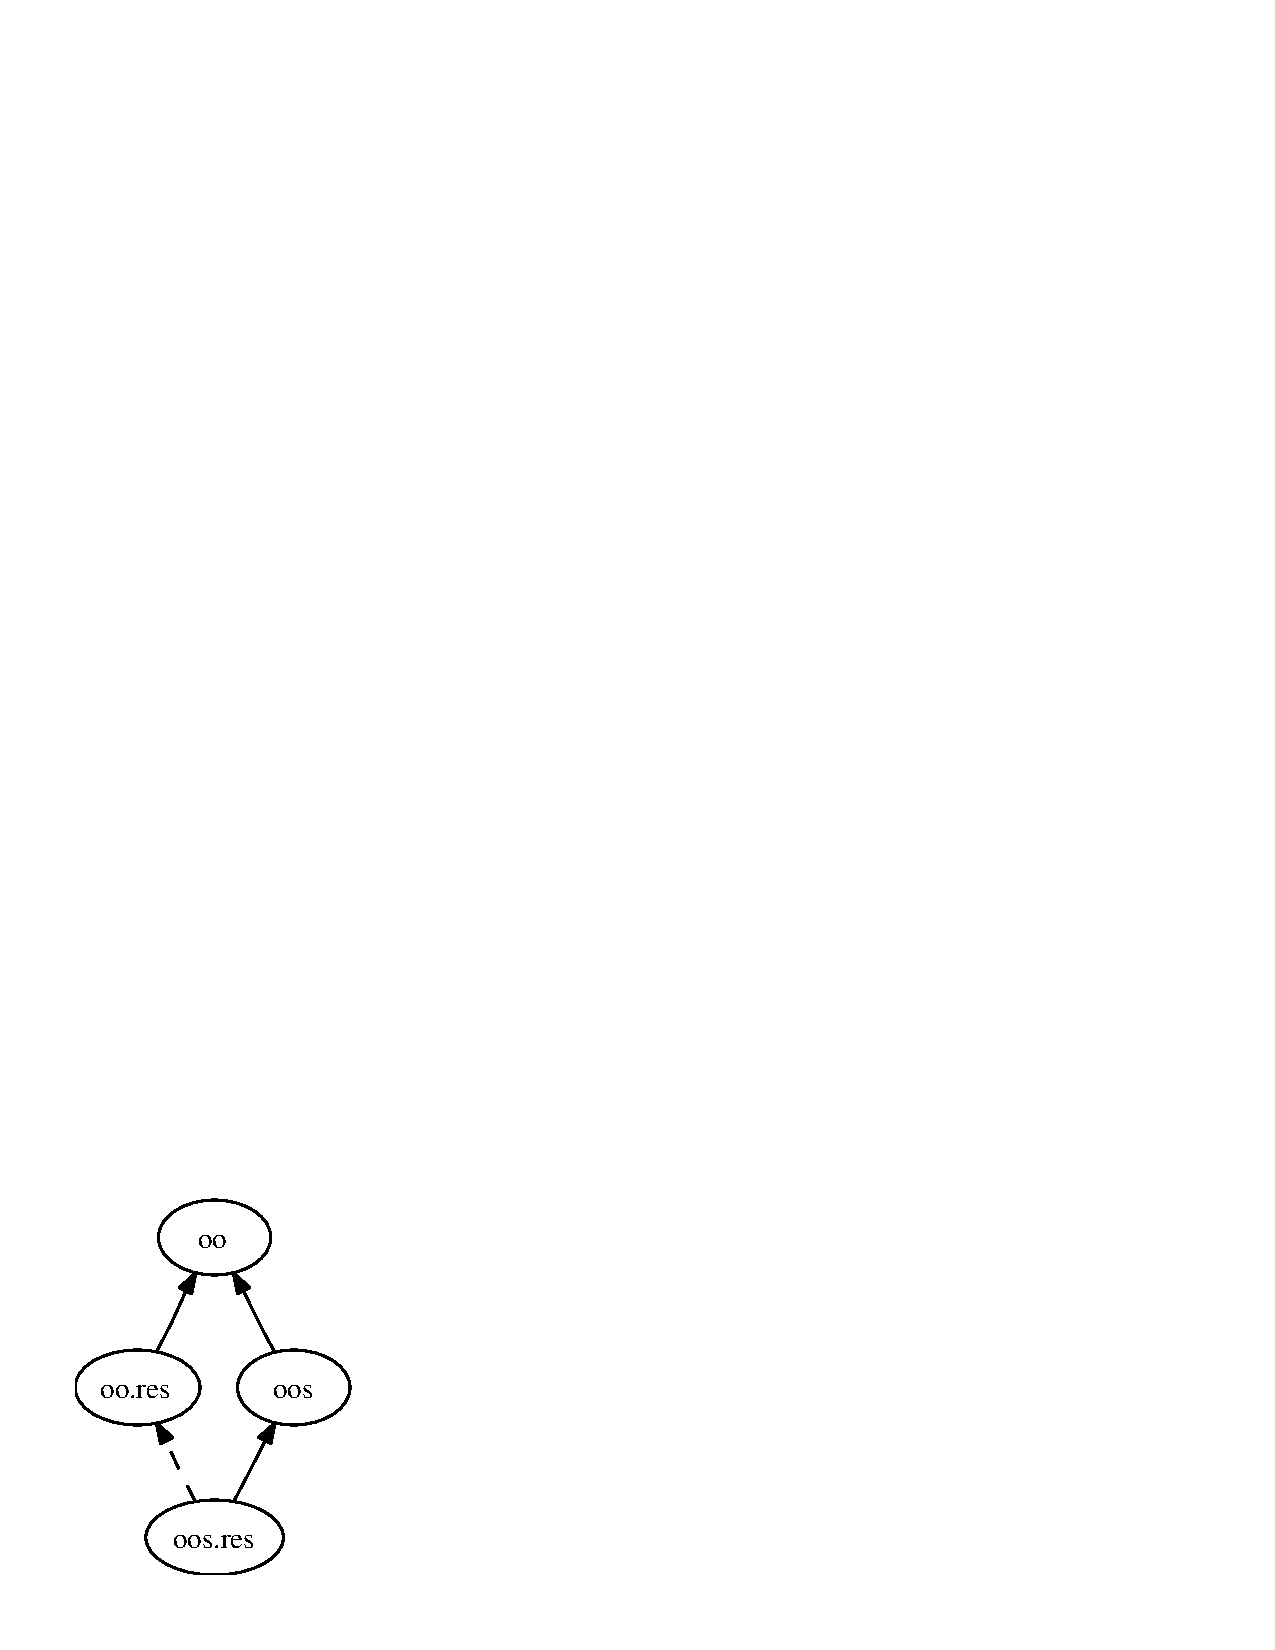
\includegraphics[width=50mm]{cloning3.pdf}
\caption{Cloning (dashed line) and delegation (solid line).  Edges point
from child to parent.}\label{fig:cloning}
\end{center}
\end{figure}

We have delegated variables
and methods and overridden both.
Thus, even with such a simple analysis, object orientation
and delegation came into play.
The reader can plainly see that smoothing and residual
analysis were not crucial to the example and this example
could be replaced with any statistical analysis including
likelihood or other estimation techniques, time series, survival
analysis, stochastic processes and so on.  The key aspect is
just that we are performing one-of analyses and do not want to
set up an elaborate class infrastructure but just want to
directly create objects to organize our calculations while
relying on delegation and dispatch to eliminate redundancy.

\subsection{Correlation, Fisher's Transform and Bootstrapping}
\label{sec:corr}

The common approach to
confidence intervals for the correlation coefficient is to
assume normality of the underlying data and then use Fisher's transform
to transform the correlation coefficient to an approximately normal
random variable.
Fisher showed that with the above normality assumption, transforming
the correlation coefficient using
the hyperbolic arc tangent function
yields a random variable
approximately distributed with an
$\frac{N(p, 1)}{\sqrt(n-3)}$ distribution.  The transformed random
variable can be used to create normal distribution confidence intervals
and the procedure can be back transformed to get confidence intervals
for the original correlation coefficient.

A more recent approach to confidence intervals for the correlation
coefficient is to use bootstrapping.  This does not require the
assumption of normality of the underlying distribution and requires
no special purpose theory devoted solely to the correlation coefficient,

Let us calculate the 95\%
confidence intervals using Fisher's transform
first.  We use \code{GNP} and \code{Unemployed} from the Longley data
set.  First we retrieve the data set and extract the required columns
into \code{x}.  Then we set \code{n} to the number of cases
and \code{pp} to the percentiles
of interest.  Finally we calculate the sample correlation and
create a function to calculate the confidence interval using
Fisher's Transform.  This function not only returns the confidence
interval but also stores it in \code{CI} in the receiver object.

\begin{Schunk}
\begin{Sinput}
> longley.ci <- proto(expr = {
+     data(longley)
+     x <- longley[, c("GNP", "Unemployed")]
+     n <- nrow(x)
+     pp <- c(0.025, 0.975)
+     corx <- cor(x)[1, 2]
+     ci <- function(.) (.$CI <- tanh(atanh(.$corx) + qnorm(.$pp)/sqrt(.$n -
+         3)))
+ })
\end{Sinput}
\end{Schunk}

Now let us repeat this analysis using the bootstrapping approach.  We
derive a new object \code{longley.ci.boot} as child of
\code{longley.ci}, setting the number of replications, \code{N}, and
defining the procedure, \code{ci} which does the actual bootstrap
calculation.

\begin{Schunk}
\begin{Sinput}
> longley.ci.boot <- longley.ci$proto({
+     N <- 1000
+     ci <- function(.) {
+         corx <- function(idx) cor(.$x[idx, ])[1, 2]
+         samp <- replicate(.$N, corx(sample(.$n, replace = TRUE)))
+         (.$CI <- quantile(samp, .$pp))
+     }
+ })
\end{Sinput}
\end{Schunk}

In the example code below the first line runs the Fisher Transform
procedure and the second runs the bootstrap procedure.  Just to check
that we have performed sufficient bootstrap iterations we rerun it in
the third line, creating a delegated object on-the-fly running its
\code{ci} method and then immediately throwing the object away.
The fact that 4,000
replications give roughly the same result as 1,000 replications
satisfies us that we have used a sufficient number of replications.

\begin{Schunk}
\begin{Sinput}
> longley.ci$ci()
\end{Sinput}
\begin{Soutput}
[1] 0.1549766 0.8464304
\end{Soutput}
\begin{Sinput}
> longley.ci.boot$ci()
\end{Sinput}
\begin{Soutput}
     2.5%     97.5%
0.2299395 0.8211854
\end{Soutput}
\begin{Sinput}
> longley.ci.boot$proto(N = 4000)$ci()
\end{Sinput}
\begin{Soutput}
     2.5%     97.5%
0.2480999 0.8259276
\end{Soutput}
\end{Schunk}

We now have the results stored in two objects nicely organized for the
future.  Note, again, that despite the simplicity of the example we
have used the features of object oriented programming, coupling the
data and methods that go together, while relying on delegation and
dispatch to avoid duplication.

\subsection{Dendrograms}
\label{sec:tree}

In \cite{Gentleman2002} there is an \proglang{S4}
example of creating a binary tree
for use as a dendrogram.  Here we directly define a binary tree with no
setup at all.  To keep it short we will create a binary tree of only
two nodes having a root whose left branch points to a leaf.  The leaf
inherits the \code{value} and \code{incr} components from the root.
The attractive feature is that the leaf be defined as a child of the
parent using \code{proto} before the parent is even finished
being defined.  Compared to the cited \proglang{S4} example where it
was necessary to create an extra class to introduce the required level of
indirection there is no need to take any similar action.

\code{tree} is the root node of the tree.  It has four components.  A
method \code{incr} which increments the \code{value} component, a
\code{..Name}, the \code{value} component itself and the left branch
\code{..left}.  \code{..left} is itself a proto object which is a
child of \code{tree}.  The leaf inherits the \code{value} component
from its parent, the root.  As mentioned, at the time we define
\code{..left} we have not even finished defining \code{tree} yet we
are able to implicitly reference the yet to be defined parent.

\begin{Schunk}
\begin{Sinput}
> tree <- proto(expr = {
+     incr <- function(., val) .$value <- .$value + val
+     ..Name <- "root"
+     value <- 3
+     ..left <- proto(expr = {
+         ..Name = "leaf"
+     })
+ })
\end{Sinput}
\end{Schunk}

Although this is a simple structure we could have embedded additional
children into \code{root} and \code{leaf} and so on recursively making
the tree or dendrogram arbitrarily complex.

Let us do some computation with this structure.  We display the
\code{value} fields in the two nodes, increment the value field in the
root and then display the two nodes again to show .that the leaf
changed too.

\begin{Schunk}
\begin{Sinput}
> cat("root:", tree$value, "leaf:", tree$..left$value, "\n")
\end{Sinput}
\begin{Soutput}
root: 3 leaf: 3
\end{Soutput}
\begin{Sinput}
> tree$incr(1)
> cat("root:", tree$value, "leaf:", tree$..left$value, "\n")
\end{Sinput}
\begin{Soutput}
root: 4 leaf: 4
\end{Soutput}
\end{Schunk}

If we increment \code{value} in \code{leaf} directly (see the example
below where we increment it by 10) then it receives its own copy of
\code{value} so from that point on \code{leaf} no longer inherits
\code{value} from \code{root}.  Thus incrementing the root by 5 no
longer increments the \code{value} field in the leaf.

\begin{Schunk}
\begin{Sinput}
> tree$..left$incr(10)
> cat("root:", tree$value, "leaf:", tree$..left$value, "\n")
\end{Sinput}
\begin{Soutput}
root: 4 leaf: 14
\end{Soutput}
\begin{Sinput}
> tree$incr(5)
> cat("root:", tree$value, "leaf:", tree$..left$value, "\n")
\end{Sinput}
\begin{Soutput}
root: 9 leaf: 14
\end{Soutput}
\end{Schunk}

\subsection{From Prototypes to Classes}
\label{sec:increment}

In many cases we will use \pkg{proto} for a design that uses prototypes
during the full development cycle.  In other cases we may use it in an
incremental way starting with prototypes but ultimately transitioning
to classes.
As shown in Section~\ref{sec:traits} the \pkg{proto} package is
powerful enough to handle class-based as well as class-free programming.
Here we illustrate this process of incremental design
starting with
concrete objects and then over time classifing them into classes,
evolving a class-based program.  \pkg{proto} provides a smooth
transition path since it can handle both the class-free and the class-based
phases -- there is no need to switch object systems part way through.
In this example, we define an object which holds a linear equation, \code{eq},
represented as a character string in terms of the unknown variable \code{x}
and a \code{print} and a \code{solve} method.  We execute the
\code{print} method
to solve it.  We also create child object \code{lineq2}
which overrides \code{eq} and execute its \code{print} method.

\begin{Schunk}
\begin{Sinput}
> lineq <- proto(eq = "6*x + 12 - 10*x/4 = 2*x", solve = function(.) {
+     e <- eval(parse(text = paste(sub("=", "-(", .$eq), ")")),
+         list(x = 0+1i))
+     -Re(e)/Im(e)
+ }, print = function(.) cat("Equation:", .$eq, "Solution:", .$solve(),
+     "\n"))
> lineq$print()
\end{Sinput}
\begin{Soutput}
Equation: 6*x + 12 - 10*x/4 = 2*x Solution: -8
\end{Soutput}
\begin{Sinput}
> lineq2 <- lineq$proto(eq = "2*x = 7*x-12+x")
> lineq2$print()
\end{Sinput}
\begin{Soutput}
Equation: 2*x = 7*x-12+x Solution: 2
\end{Soutput}
\end{Schunk}

We could continue with enhancements but at this point we decide that we
have a general case and so wish
to abstract \code{lineq} into a class.  Thus we define a trait,
\code{Lineq}, which is just \code{lineq} minus \code{eq} plus
a constructor \code{new}.  The key difference between \code{new}
and the usual \code{proto} function
is that with \code{new} the initialization of \code{eq} is mandatory.
Having completed this definition
we instantiate an object of
class/trait \code{Lineq} and execute it.

\begin{Schunk}
\begin{Sinput}
> Lineq <- lineq
> rm(eq, envir = Lineq)
> Lineq$new <- function(., eq) proto(., eq = eq)
> lineq3 <- Lineq$new("3*x=6")
> lineq3$print()
\end{Sinput}
\begin{Soutput}
Equation: 3*x=6 Solution: 2
\end{Soutput}
\end{Schunk}

Note how we have transitioned from a prototype style of programming
to a class-based style of programming all the while staying within
the \pkg{proto} framework.

\section{Summary} \label{sec:summary}

\subsection{Benefits}
\label{sec:benefits}

The key benefit of the \pkg{proto} package is to provide
access to a style of programming that has not been conveniently
accessible within \proglang{R} or any other mainstream language today.

\pkg{proto} can be used in two key ways: class-free object oriented programming
and class-based object oriented programming.

A key application for \pkg{proto} in class-free programming is to wrap the code
and data for each run of a particular statistical study into an object for
purposes of organization and reproducibility.  It provides such organization
directly and without the need and overhead of class definitions
yet still provides the
inheritance and dispatch advantages of object oriented programming.
We provide examples of this style of programming in
Section~\ref{sec:smooth}
and
Section~\ref{sec:corr}.
A third example in
Section~\ref{sec:tree} illustrates a beneficial use of \pkg{proto} with
recursive data structures.

Another situation where prototype programming is of interest is in the initial
development stages of a program.  In this case, the design may not be fully
clear so it is more convenient to create concrete objects individually rather
than premature abstractions through classes.  The \code{graph.proto}
function can be used to generate visual representations of the object
tree suggesting classifications of objects so that
as the program evolves the general case becomes clearer and
in a bottom up fashion the objects are incrementally abstracted into
classes.  In this case,
\pkg{proto} provides a smooth transition path since it not only supports
class-free programming but, as explained in the Section~\ref{sec:traits}, is
sufficiently powerful to support class-based programming, as well.


\subsection{Conclusion}
\label{sec:conclusion}

The package \pkg{proto} provides an \proglang{S3} subclass of the
\code{environment} class for constructing and manipulating object
oriented systems without classes.  It can also emulate classes even
though classes are not a primitive structure.  Its key design goals
are to provide as simple and as thin a layer as practically possible
while giving the user convenient access to this alternate object
oriented paradigm.  This paper describes, by example, how prototype
programming can be carried out in \proglang{R} using \pkg{proto} and
illustrates such usage.  Delegation, cloning traits and general
manipulation and incremental development are all reviewed by example.

\section*{Computational details}
\label{sec:compute}

The results in this paper were obtained using \proglang{R} 2.1.0 with
the package \pkg{proto} 0.3--2. \proglang{R} itself and the
\pkg{proto} package are available from CRAN at
\url{http://CRAN.R-project.org/}.  The GraphViz software is available
from \url{http://www.graphviz.org}.

\phantomsection
\addcontentsline{toc}{section}{References}
\bibliography{proto}
%

%\VignetteIndexEntry{proto: An R Package for Prototype Programming}
%\VignetteDepends{}
%\VignetteKeywords{object oriented, prototype programming, S3, R}
%\VignettePackage{proto}


\documentclass[nojss]{jss}
\usepackage{Sweave}
\DeclareGraphicsExtensions{.pdf, .eps, .png}



\newlength{\half}
\setlength{\half}{70mm}

\author{Louis Kates\\GKX Associates Inc. \And
        Thomas Petzoldt\\Technische Universit\"at Dresden}
\Plainauthor{Louis Kates, Thomas Petzoldt}

\title{\pkg{proto}: An \proglang{R} Package for Prototype Programming}
%% \Shorttitle{\pkg{proto}: An \proglang{R} Package for Prototype Programming}

\Plaintitle{proto: An R Package for Prototype Programming}

\Keywords{prototype programming, delegation, inheritance, clone,
  object orientated, \proglang{S3}, \proglang{R}}
\Plainkeywords{object oriented, prototype programming, S3, R}

\Abstract{

  \pkg{proto} is an \proglang{R} package which facilitates a style
  of programming known as prototype
  programming.  Prototype programming is a type of object
  oriented programming in which there are no classes.
  \pkg{proto} is simple yet retains the object oriented features of
  delegation (the prototype counterpart to inheritance)
  and object oriented  dispatch.  \code{proto} can be used
  to organize the concrete data and procedures in statistical studies
  and other applications
  without the necessity of defining classes while still providing convenient
  access to an object oriented style of programming.  Furthermore, it
  can be used in a class-based style as well so that incremental design can
  begin with defining the concrete objects and later transition to abstract
  classes, once the general case is understood, without having to change to
  object-oriented frameworks.
  The key goals of the package are to integrate into \proglang{R}
  while providing nothing more than a thin layer on top of it.
}

\hyphenation{ma-ni-pu-lating}

\begin{document}
\input{proto-concordance}




\section{Introduction} \label{sec:intro}

\subsection[Object Oriented Programming in R]{Object Oriented Programming in \proglang{R}}
\label{sec:oo}

The \proglang{R} system for statistical computing
\citep[\url{http://www.R-project.org/}]{Rcore2005} ships with two
systems for object oriented programming referred to as \proglang{S3}
and \proglang{S4}.  With the increased interest in object oriented
programming within \proglang{R} over the last years additional object
oriented programming packages emerged.  These include the \pkg{R.oo}
package \citep{Bengtsson2003} and the \pkg{OOP} package
\citep[\url{http://www.omegahat.net/OOP/}]{Rnews:Chambers+Lang:2001a}.
All these packages have the common thread that they use
classes as the basis of inheritance.  When a message is sent to an
object the class of the object is examined and that class determines the
specific function to be executed. In prototype programming there
are no classes making it simple yet it retains much of the power of
class-based programming.  In the fact, \pkg{proto} is so simple that
there is only one significant new routine name, \code{proto}.  The
other routines are just the expected support routines such as
\code{as.proto} to coerce objects to proto objects, \code{\$} to
access and set proto object components and \code{is.proto} to check
whether an object is a proto object.  In addition, \code{graph.proto}
will generate a graphical ancestor tree showing the parent-child
relationships among generated \code{proto} objects.

The aim of the package is to provide a lightweight layer for prototype
programming in \proglang{R} written only in \proglang{R} leveraging the
existing facilities of the language rather than adding its own.

\subsection{History}
\label{sec:history}

The concept of
prototype programming
\citep{Lieberman1986, Taivalsaari1996a, Noble1999}
has developed over a number of years with the \proglang{Self}
language \citep{Agesen1992}
being the key evolved programming language to demonstrate
the concept.  In statistics, the \proglang{Lisp}-based
\proglang{LispStat} programming language \citep{Tierney1990} was
the first and possibly only statistical system to feature prototype
programming.

Despite having been developed over 20 years ago, and some attempts to
enter the mainstream (e.g.  \proglang{Newtonscript}
on the Newton computer, which
is no longer available, and \proglang{Javascript} where
it is available but whose
domain of application largely precluses use of prototype programming)
prototype programming is not well known due to lack of language
support in popular programming languages such as \proglang{C} and
\proglang{Java}.  It tends
to be the domain of research languages or \proglang{Lisp}.

Thus the
the availability of a popular language,
\proglang{R} \footnote{Some indications of the popularity of R are
the high volume mailing lists, international development team, the
existence of over 500 addon packages, conferences and numerous books
and papers devoted to R.},
that finally does provide the key infrastructure
is an important development.

This work grew out of the need to organize multiple scenarios of model
simulations in ecological modelling \citep{Rnews:Petzoldt:2003} and
was subsequently generalized to the present package.  A number of
iterations of the code, some motivated by the ever increasing feature
set in \proglang{R}, resulted in a series of utilities and ultimately
successive versions of an \proglang{R} package developed over the last
year.  An initial version used \proglang{R} lists as the basis of the
package.  Subsequently the package was changed to use \proglang{R}
environments.  The first version to use environments stored the
receiver object variable in a proxy parent environment which was
created on-the-fly at each method call.  The present version of
the \pkg{proto} package passes the receiver object through the argument list,
while hiding this from the caller.  It defines the \code{proto} class
as a subclass of the \code{environment} class so that
functionality built into \proglang{R} for the environment class is
automatically inherited by the \code{proto} class.

\subsection{Overview}
\label{sec:overview}

It is assumed that the reader has some general
familiarity with object oriented programming concepts and with
\proglang{R}.

The paper will proceed primarily by example focusing on illustrating
the package \code{proto} through such demonstration.  The remainder of
the paper is organized as follows: Section~\ref{sec:proto-class}
explains how \code{"proto"} objects are created and illustrates the
corresponding methods for setting and getting components.  It further
discusses how object oriented delegation (the prototype programming
analogue of inheritance) is handled and finally discusses the
internals of the package.  This section uses small examples chosen for
their simplicity in illustrating the concepts.  In
Section~\ref{sec:examples} we provide additional examples of prototype
programming in action.  Four examples are shown.  The first involves
smoothing of data.  Secondly we demonstrate the calculation of
correlation confidence intervals using classical (Fisher Transform)
and modern (bootstrapping) methods.  Thirdly we demonstrate the
development of a binary tree as would be required for a dendrogram.
Fourthly, we use the solution of linear equations to illustrate
program evolution from object-based to class-based, all
within the \pkg{proto} framework.
Section~\ref{sec:summary} gives a few summarizing remarks.  Finally,
an appendix provides a reference card that summarizes the
functionality contained in \pkg{proto} in terms of its constituent
commands.

%% \pagebreak[4]

\section[The class "proto" and its methods]{The class \code{"proto"} and its methods}
\label{sec:proto-class}

\subsection[Creation of "proto" objects]{Creation of \code{"proto"} objects}
\label{sec:proto}

In this section we shall show, by example, the creation of two
prototype objects and related operations.  The simple idea is that
each \code{"proto"} object is a set of components: functions (methods)
and variables, which are tightly related in some way.

A prototype object is an environment holding the variables and
methods of the object. \footnote{In particular this implies that
\code{"proto"} objects have single inheritance, follow ordinary
environment scoping rules and have mutable state as environments
do.}

A prototype object is created using the constructor function
\code{proto} (see Appendix~\ref{sec:ref} at the end of this paper or
\pkg{proto} package help for complete syntax of commands).

\begin{Scode}
addProto <- proto( x = rnorm(5), add = function(.) sum(.$x) )
\end{Scode}

In this simple example, the \code{proto} function defines two
components: a variable \code{x} and a method \code{add}.  The variable
\code{x} is a vector of 5 numbers and the method sums those numbers.
The \code{proto} object \code{addProto} contains the variable and the
method.  Thus the \code{addProto} \code{proto} object can be used to compute
the sum of the values stored in it.
As shown with the \code{add} method in this example, formal argument
lists of methods must always have a first argument of dot
(i.e. \code{.})  which signifies the object on which the method is
operating.  The dot refers to the current object in the same way that
a dot refers to the current directory in UNIX.  Within the method one
must refer to other variables and methods in the object by prefacing
each with \code{.\$}.  For example, in the above we write
\code{sum(.\$x)}.  Finally, note that the data and the method are very
closely related.  Such close coupling is important in order to create
an easily maintained system.

To illustrate the usage of \code{proto}, we first load the package and
set the random seed to make the examples in this paper exactly
reproducible.

\begin{Schunk}
\begin{Sinput}
> library(proto)
> set.seed(123)
\end{Sinput}
\end{Schunk}

Then, we create the \code{proto} object from above
and call its \code{add} method.
\begin{Schunk}
\begin{Sinput}
> addProto <- proto(x = rnorm(5), add = function(.) sum(.$x))
> addProto$add()
\end{Sinput}
\begin{Soutput}
[1] 0.9678513
\end{Soutput}
\end{Schunk}
We also create another object, \code{addProto2}
with a different \code{x} vector and
invoke its \code{add} method too.
\begin{Schunk}
\begin{Sinput}
> addProto2 <- addProto$proto(x = 1:5)
> addProto2$add()
\end{Sinput}
\begin{Soutput}
[1] 15
\end{Soutput}
\end{Schunk}
In the examples above, we created a prototype object \code{addProto}
and then called its \code{add} method as just explained.
The notation \code{addProto\$add}
tells the system to look for the \code{add} method
in the \code{addProto} object.  In the expression \code{addProto\$add},
the \code{proto} object to the left
of the dollar sign, \code{addProto} here, is referred to as the
\emph{receiver} object.  This expression
also has a second purpose which is to
pass the receiver object implicitly as the first argument of \code{add}.
Note that we called \code{add} as if it had zero arguments but, in fact,
it has one argument because the receiver is automatically and implicitly
supplied as the first argument.  In general,
the notation \code{object\$method(arguments)} is
used to invoke the indicated method of the receiver object using the
object as the implicit first argument along with the indicated
arguments as the subsequent arguments.
As with the \code{addProto} example, the receiver
object not only determines where to find the
method but also is implicitly passed to the method through
the first argument.  The motivation for this notation
is to relieve the user of
specifying the receiver object twice:
once to locate the method in the object and a second
time to pass the object itself to the method.
The \code{\$} is overloaded by the \code{proto}
class to automatically do both with one reference to the receiver object.
Even though, as with the \code{addProto} example, the first
argument is not listed in the call
it still must be listed among the formal arguments
in the definition of the method.  It
is conventional to use
a dot \code{.} as the first formal argument in the method/function
definition.  That is, we call \code{add} using \code{addProto\$add()}
displaying zero arguments
but we define \code{add} in \code{addProto} displaying
one argument \code{add <- function(.)}, the dot.

In this example,
we also created a second object, \code{addProto2},
which has the first object, \code{addProto} as its parent.
Any reference to a
component in the second object that is unsuccessful will cause
search to continue in the parent.  Thus the call \code{addProto2\$add()}
looks for \code{add} in \code{addProto2} and not finding it there
searches its parent, \code{addProto}, where it is, indeed, found.
\code{add} is invoked with the receiver object, \code{addProto2}, as
the value of dot.
The call \code{addProto2\$add()} actually causes the \code{add}
in \code{addProto} to run but it still uses the \code{x} from
\code{addProto2} since dot (\code{.}) is \code{addProto2} here
and \code{add} references \code{.\$x}.
Note that the reference to \code{.\$x} in the
\code{add} found in \code{addProto}
does not refer to the \code{x} in \code{addProto} itself.
The \code{x} in \code{addProto2} has overridden the \code{x} in its parent.
This point is important so the reader should take care to absorb this
point.

This simple example already shows the key elements of the system
and how \emph{delegation} (the prototype programming term for inheritance)
works without classes.

We can add new components or replace components in an object and
invoke various methods like this:
\begin{Schunk}
\begin{Sinput}
> addProto2$y <- seq(2, 10, 2)
> addProto2$x <- 1:10
> addProto2$add3 <- function(., z) sum(.$x) + sum(.$y) + sum(z)
> addProto2$add()
\end{Sinput}
\begin{Soutput}
[1] 55
\end{Soutput}
\begin{Sinput}
> addProto2$add3(c(2, 3, 5))
\end{Sinput}
\begin{Soutput}
[1] 95
\end{Soutput}
\begin{Sinput}
> addProto2$y
\end{Sinput}
\begin{Soutput}
[1]  2  4  6  8 10
\end{Soutput}
\end{Schunk}

In this example, we insert variable \code{y} into the object \code{addProto2}
with a value of \code{seq(2,10,2)},
reset variable \code{x} to a new value and insert a new method,
\code{add3}. Then we invoke
our two methods and display \code{y}.  Again, note that in the case of
\code{protoAdd2\$add} the \code{add} method is not present in
\code{protoAdd2} and so search continues to the parent \code{addProto}
where it is found.

\subsection{Internals}
\label{sec:internals}

So far, we have used simple examples to illustrate the basic manipulation
of objects: construction, getting and setting components and method
invocation.  We now discuss the internals of the package and how it relates
to \proglang{R} constructs.
\code{proto} is actually an \proglang{S3} class which is a subclass
of the \code{environment} class.  Every \code{proto} object is an
environment and its class is \code{c("proto", "environment")}.  The \code{\$}
accessor is similar to the same accessor in environments except it will
use the \proglang{R} \code{get} function to
search up parent links if it cannot otherwise find the object (unlike
environments).  When accessing a method, \code{\$}
automatically supplies the
first argument to the method
unless the object is \code{.that} or \code{.super}.  \code{.that}
is a special variable which \code{proto} adds to every \code{proto} object
denoting the object itself.  \code{.super} is also added to every
proto object and is the parent of \code{.that}.  \code{.that}
and \code{.super} are normally used
within methods of an object to refer to other components of the same
or parent object, respectively,
as opposed to the receiver (\code{.}).  For example,
suppose we want \code{add} in \code{addProto2} to add the elements
of \code{x} together and the elements of
\code{y} together and then add these two sums.  We could redefine add like this:

\begin{Schunk}
\begin{Sinput}
> addProto2$add <- function(.) .super$add(.) + sum(.$y)
\end{Sinput}
\end{Schunk}

making use of the \code{add} already defined in the parent.
One exception should be noted here.  When one uses \code{.super},
as above, or \code{.that} to specify a method then the receiver
object must be explicitly specified
in argument one (since in those cases the receiver
is possibly different than
\code{.super} or \code{.that} so the system cannot automatically supply it
to the call.)

Setting a value is similar to the corresponding operation for
environments except that any function, i.e method, which is
inserted has its environment set to the environment of the object
into which it is being inserted.  This is necessary so that such
methods can reference \code{.that} and \code{.super} using
lexical scoping.

In closing this section a few points should be re-emphasized and
expanded upon.  A
\code{proto} object is an environment whose parent object is the
parent environment of the \code{proto} object.  The methods in the \code{proto}
objects are ordinary functions that have the containing object as their
environment.

The \proglang{R} \code{with} function can be used with environments and
therefore can be used with \code{proto} objects since \code{proto}
objects are environments too.  Thus \code{with(addProto, x)} refers
to the variable \code{x} in \code{proto} object \code{addProto}
and \code{with(addProto, add)} refers to the method \code{add}
in the same way.  \code{with(addProto, add)(addProto)} can be used
to call \code{add}.  These constructs all follow from their corresponding
use in environments from which they are inherited.

Because the \code{with} expressions are somewhat verbose, two common
cases can be shortened using the \code{\$} operator.  \code{addProto\$x}
can be used to refer to variable \code{x} in \code{proto} object
\code{addProto} and has the same meaning as \code{with(addProto, x)}.
In particular like \code{with} but
unlike the the behavior of the \code{\$} operator on
environments, when used with \code{proto} objects, \code{\$} will
search not only the object itself but also its ancestors.
Similarly \code{addProto\$add()} can be used to call
method \code{add} in \code{addProto} also searching through ancestors
if not found in \code{addProto}.  Note that \code{addProto\$add}
returns an object of class

\code{c("instantiatedProtoMethod", "function")}
which is derived from \code{add} such that the first argument,
the \code{proto} object,
is already inserted.  Note that there is a \code{print} method for
class \code{"instantiatedProtoMethod"} so printing such objects will
display the underlying function but returning such objects
is not the same as returning the function without slot one inserted.
Thus, if one wants exactly the original \code{add}
as a value one should use \code{with(addProto, add)} or
\code{addProto\$with(add)}.

Within a method, if a variable is referred to without
qualification simply as \code{x}, say, then  its meaning  is
unchanged from how it is otherwise used in \proglang{R} and
follows the same scope rules as any variable to resolve its name.  If it is
desired that the variable have object scope, i.e. looked up
in the receiver object and its ancestors, then \code{.\$x}
or similar \code{with} notation, i.e. \code{with(., x)}, should be used.
Similarly \code{.\$f(x)} calls
method \code{f} automatically inserting the receiver object
into argument one and using \code{x} for argument two.  It
looks for \code{f} first in the receiver object and then its
ancestors.

\subsection{Traits}
\label{sec:traits}

Let us look at the definition of a child object once again.
In the code below,
\code{addProto} is the previously defined parent object
and the expression \code{addProto\$proto(x = 1:5)} defines
a child object of \code{addProto} and assigns it to variable
\code{addProto2a}.

\begin{Schunk}
\begin{Sinput}
> addProto2a <- addProto$proto(x = 1:5)
> addProto2a$add()
\end{Sinput}
\begin{Soutput}
[1] 15
\end{Soutput}
\end{Schunk}

That is, \code{proto} can be used to create a new child of
an existing object by writing the
parent object on the left of the \code{\$} and
\code{proto} on its right.  Any contents to
be added to the new child are listed in arguments of \code{proto}
as shown.

For example, first let us create a class-like structure.  In the
following \code{Add} is an object that behaves very much like a class
with an \code{add} method and a method \code{new} which constructs
new objects.  In the line creating object \code{add1} the expression
\code{Add\$new(x = 1:5)} invokes the \code{new} constructor of the
receiver object \code{Add}. The method \code{new} has an argument of
\code{x = 1:5} which defines an \code{x} variable in the \code{add1}
object being instantiated. We similarly create another object
\code{add2}.

\begin{Schunk}
\begin{Sinput}
> Add <- proto(add = function(.) sum(.$x), new = function(., x) .$proto(x = x))
> add1 <- Add$new(x = 1:5)
> add1$add()
\end{Sinput}
\begin{Soutput}
[1] 15
\end{Soutput}
\begin{Sinput}
> add2 <- Add$new(x = 1:10)
> add2$add()
\end{Sinput}
\begin{Soutput}
[1] 55
\end{Soutput}
\end{Schunk}

An object which contains only methods and variables that are
intended to be shared by all its children (as opposed to an
object whose purpose is to have its own methods and variables)
is known as a \emph{trait} \citep{Agesen1992}.  It
is similar to a class in class-based
object oriented programming.
Note that the objects \code{add1} and \code{add2} have the trait
\code{Add} as their parent.  We could implement subclass-like and
superclass-like objects by simply defining similar trait objects to
be the parent or child of \code{Add}.  For example, suppose we
want a class which calculates the sum of the logarithms of the data.  We
could define:

\begin{Schunk}
\begin{Sinput}
> Logadd <- Add$proto(logadd = function(.) log(.$add()))
> logadd1 <- Logadd$new(1:5)
> logadd1$logadd()
\end{Sinput}
\begin{Soutput}
[1] 2.70805
\end{Soutput}
\end{Schunk}

Here the capitalized objects are traits.
\code{Logadd} is a trait.  It is a child of \code{Add}
which is also a trait.  \code{logadd1} is an ordinary object,
not a trait.
One possible design is to create a tree of traits and other objects
in which the leaves are ordinary objects and the remaining nodes
are traits.  This would closely correspond to class-based
object oriented programming.

Note that the delegation of methods from
one trait to another as in
\code{new} which is inherited by \code{Logadd} from \code{Add}
is nothing more than the same mechanism by which traits delegate
methods to
objects since, of course, traits are just objects no different
from any other object other than by the conventions we impose on them.
This unification of subclassing and instantiation beautifully
shows the simplification that prototype programming represents.

\subsection{Utilities}
\label{sec:utilities}
The fact that method calls automatically insert the first argument
can be used to good effect in leveraging existing \proglang{R}
functions while allowing an object-oriented syntax.

For example, \code{ls()} can be used to list the components of
\code{proto} objects:

\begin{Schunk}
\begin{Sinput}
> addProto$ls()
\end{Sinput}
\begin{Soutput}
[1] "add" "x"
\end{Soutput}
\end{Schunk}

Functions like:

\begin{Schunk}
\begin{Sinput}
> addProto$str()
> addProto$print()
> addProto$as.list()
> addProto2a$parent.env()
\end{Sinput}
\end{Schunk}

show additional information about the elements.  \code{eapply}
can be used to explore more properties such as the
the length of each component of an object:

\begin{Schunk}
\begin{Sinput}
> addProto$eapply(length)
\end{Sinput}
\end{Schunk}

Another example of some interest in any object oriented system
which allows multiple references to one single object is that
object identity
can be tested using the respective base function:

\begin{Schunk}
\begin{Sinput}
> addProto$identical(addProto2)
\end{Sinput}
\begin{Soutput}
[1] FALSE
\end{Soutput}
\end{Schunk}

\code{proto} does contain a special purpose \code{str.proto} function
but in the main it
is important to notice here, that
\code{proto} has no code that is specific to \code{ls} or
any of the other ordinary \proglang{R}
functions listed.  We are simply making use of the
fact that \code{obj\$fun(...)} is transformed into \code{get("fun",
obj)(obj, ...)} by the proto \code{\$} operator.  For example, in the
case of \code{addProto\$ls()} the system looks for \code{ls} in object
\code{addProto}.  It cannot find it there so it looks to its parent,
which is the global environment.  It does not find it there so it
searches the remainder of the search path, i.e. the path shown by
running the \proglang{R} command \code{search()}, and finally finds it
in the base package, invoking it with an argument of \code{addProto}.
Since all \code{proto} objects are also environments
\code{ls(addProto)} interprets \code{addProto} as an environment and
runs the \code{ls} command with it.  In the \code{ls} example there
were no arguments other than \code{addProto}, and even that one was
implicit, but if there were
additional arguments then they would be passed as shown in the
\code{eapply} and \code{identical} examples above.

\subsection{Plotting}
\label{sec:plot}

The \code{graph.proto} function can be used to create
graphs that can be rendered by the \code{Rgraphviz} package
creating visual representations of ancestor trees (figure
\ref{fig:proto-dot}).
That package provides an interface to the
\proglang{GraphViz} \code{dot} program \citep{Ganser+North:1999}.

\code{graph.proto} takes three arguments, all of which are
usually omitted.  The first argument is a \code{proto} object
(or an environment) out of which all contained \code{proto} objects
and their parents (but not higher order ancestors) are graphed.
If it is omitted, the current environment is assumed.
The second argument is a graph (in the sense of the \code{graph}
package) to which the nodes and edges are added.  If it is omitted
an empty graph is assumed.  The last argument is a logical variable
that specifies the orientation of arrows.  If omitted arrows are
drawn from children to their parents.


\input{proto-dot}

\begin{figure}[htbp]
\begin{center}
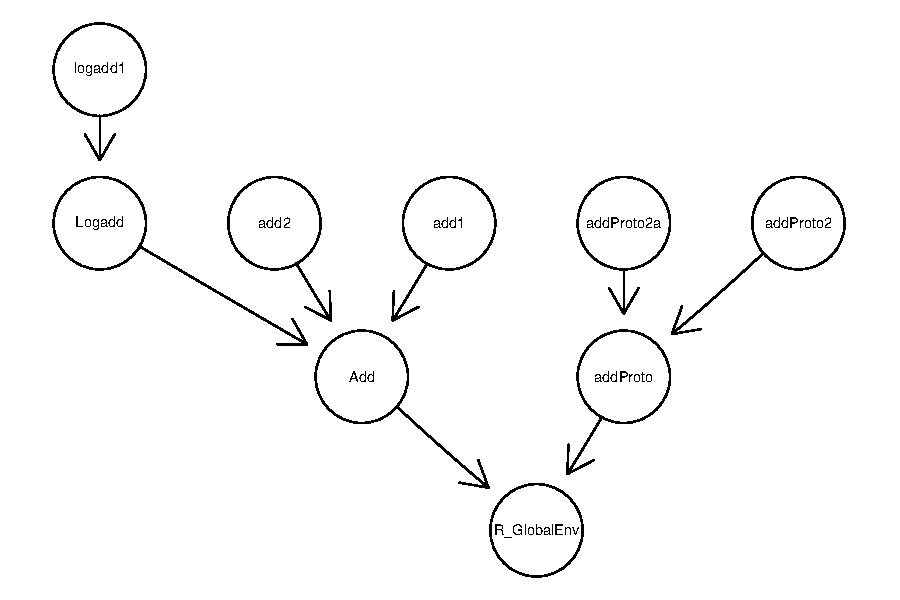
\includegraphics{proto-dot}
\caption{\label{fig:proto-dot} Ancestor tree generated using graph.proto. Edges
point from child to parent.}
\end{center}
\end{figure}

\pagebreak[4]

\section{Examples}
\label{sec:examples}

\subsection{Smoothing}
\label{sec:smooth}

In the following we create a \code{proto} object named \code{oo}
containing a vector of data \code{x} (generated from a simulated
autoregressive model) and time points
\code{tt}, an intermediate result
\code{x.smooth}, some plotting parameters \code{xlab}, \code{ylab},
\code{pch}, \code{col} and three methods \code{smooth}, \code{plot}
and \code{residuals} which smooth the data, plot the data and
calculate residuals, respectively.  We also define \code{..x.smooth}
which holds intermediate results.  Names beginning with two dots
prevent them from being delegated to children.  If we override
\code{x} in a child we would not want an out-of-sync \code{x.smooth}.
Note that the components of an object can be specified using a code
block in place of the argument notation we used previously in the
\code{proto} command.

\begin{Schunk}
\begin{Sinput}
> oo <- proto(expr = {
+     x <- rnorm(251, 0, 0.15)
+     x <- filter(x, c(1.2, -0.05, -0.18), method = "recursive")
+     x <- unclass(x[-seq(100)]) * 2 + 20
+     tt <- seq(12200, length = length(x))
+     ..x.smooth <- NA
+     xlab <- "Time (days)"
+     ylab <- "Temp (deg C)"
+     pch <- "."
+     col <- rep("black", 2)
+     smooth <- function(., ...) {
+         .$..x.smooth <- supsmu(.$tt, .$x, ...)$y
+     }
+     plot <- function(.) with(., {
+         graphics::plot(tt, x, pch = pch, xlab = xlab, ylab = ylab,
+             col = col[1])
+         if (!is.na(..x.smooth[1]))
+             lines(tt, ..x.smooth, col = col[2])
+     })
+     residuals <- function(.) with(., {
+         data.frame(t = tt, y = x - ..x.smooth)
+     })
+ })
\end{Sinput}
\end{Schunk}

Having defined our \code{proto} object we can inspect it, as shown
below, using
\code{print} which is automatically invoked if the
name of the object, \code{oo}, is entered on a line by itself.
In this case, there is no proto print method so we inherit the
environment print method which displays the environment hash code.
Although it produces too much output to show here,
we could have displayed a
list of the entire contents of the object \code{oo}
via \code{oo\$as.list(all.names = TRUE)}.
We can get a list of the names of the
components of the object using \code{oo\$ls(all.names = TRUE)} and will look
at the contents of one component, \code{oo\$pch}.

\begin{Schunk}
\begin{Sinput}
> oo
\end{Sinput}
\begin{Soutput}
<environment: 0x01fbd8c8>
attr(,"class")
[1] "proto"       "environment"
\end{Soutput}
\begin{Sinput}
> oo$ls(all.names = TRUE)
\end{Sinput}
\begin{Soutput}
 [1] "..x.smooth" ".super"     ".that"      "col"        "pch"
 [6] "plot"       "residuals"  "smooth"     "tt"         "x"
[11] "xlab"       "ylab"
\end{Soutput}
\begin{Sinput}
> oo$pch
\end{Sinput}
\begin{Soutput}
[1] "."
\end{Soutput}
\end{Schunk}

Let us illustrate a variety of manipulations.  We will set up the
output to plot 2 plots per screen using \code{mfrow}.  We change the
plotting symbol, smooth the data, invoke the \code{plot} method to
display a plot of the data and the smooth and then plot the residuals
in the second plot (figure \ref{fig:proto-smooting03}).


\input{proto-smoothing03}

\begin{figure}[h!]
\begin{center}
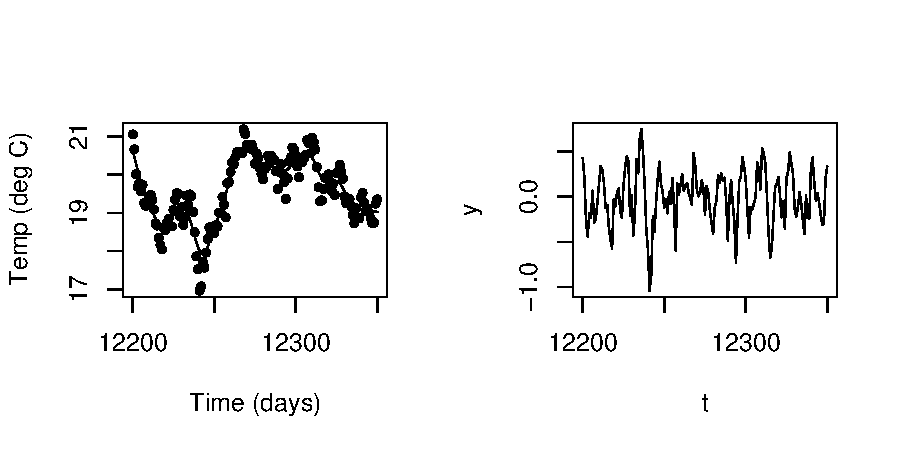
\includegraphics[width=\textwidth]{proto-smoothing03}
\end{center}
\caption{Data and smooth from \code{oo\$plot()} (left) and plot of
\code{oo\$residuals()} (right).}
\label{fig:proto-smooting03}
\end{figure}


Now let us illustrate the creation of a child object and delegation.
We create a new child object of \code{oo} called \code{oo.res}.  We
will override the \code{x} value in its parent by setting \code{x} in
the child to the value of the residuals in the parent.  We will also
override the \code{pch} and \code{ylab} plotting parameters.  We will
return to 1 plot per screen and run \code{plot} using the
\code{oo.res} object as the receiver invoking the \code{smooth} and
\code{plot} methods (which are delegated from the parent \code{oo})
with the data in the child (figure \ref{fig:smoothing04}).

\input{proto-smoothing04}
% \begin{figure}[tp]
\begin{figure}[h!]
\begin{center}
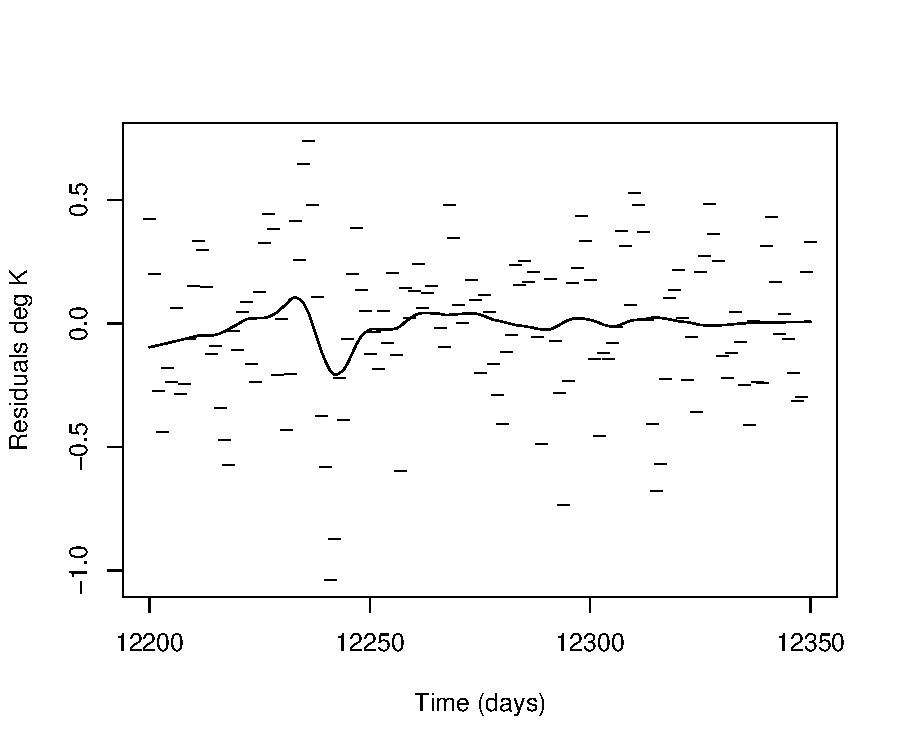
\includegraphics[width=\half]{proto-smoothing04}
\end{center}
\caption{Output of \code{oo.res\$plot()}.
\code{oo.res\$x} contains the residuals from \code{oo}.}
\label{fig:smoothing04}
\end{figure}
Now we make use of delegation to change the parent
and child in a consistent way with respect to certain plot characteristics.
We have been using a numeric time axis.
Let us interpret these numbers as the number of days since the Epoch,
January 1, 1970, and let us also change the plot colors.

\begin{Schunk}
\begin{Sinput}
> oo$tt <- oo$tt + as.Date("1970-01-01")
> oo$xlab <- format(oo.res$tt[1], "%Y")
> oo$col <- c("blue", "red")
\end{Sinput}
\end{Schunk}


We can introduce a new method, \code{splot}, into
the parent \code{oo} and have it automatically
inherited by its children.  In this example
it smooths and then plots and we use it with
both \code{oo} and \code{oo.res} (figure \ref{fig:smoothing06}).


\input{proto-smoothing06}

\begin{figure}[tbp]
\begin{center}
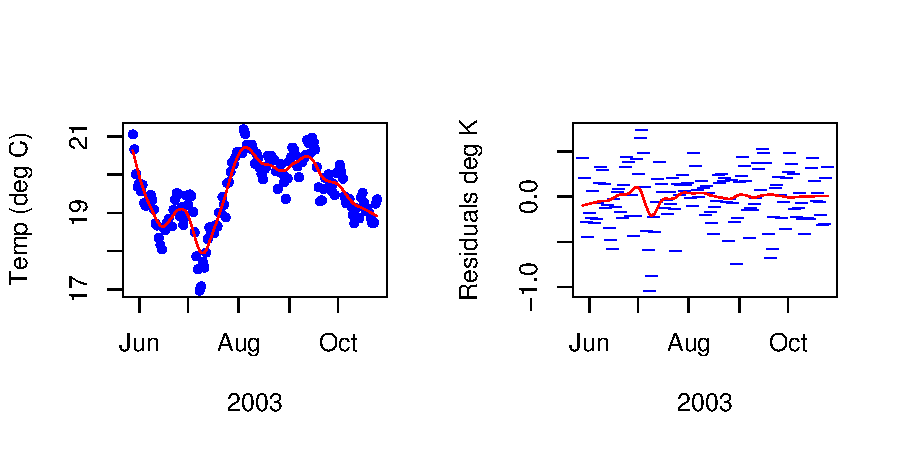
\includegraphics[width=\textwidth]{proto-smoothing06}
\caption{Plotting options and \code{splot} function applied
to both parent (left) and child (right) object}
\label{fig:smoothing06}
\end{center}
\end{figure}

Numerous possibilities exist to make use of the
mechanisms shown, so one may create different child objects, apply
different smoothing parameters, overwrite the smoothing function with
a lowess smoother and finally compare fits and residuals.

Now lets change the data and repeat the analysis.  Rather than
overwrite the data we will preserve it in \code{oo} and create a child
\code{oos} to hold an analysis with sinusoidal data.

\begin{Schunk}
\begin{Sinput}
> oos <- oo$proto(expr = {
+     tt <- seq(0, 4 * pi, length = 1000)
+     x <- sin(tt) + rnorm(tt, 0, 0.2)
+ })
> oos$splot()
\end{Sinput}
\end{Schunk}

Lets perform the residual analysis with \code{oos}.
We will make a deep copy of \code{oo.res}, i.e. duplicate its
contents and not merely delegate it, by copying \code{oo.res}
to a list from which we create the duplicate, or cloned,
\code{proto} object (figure \ref{fig:smoothing10} and \ref{fig:cloning}):

\begin{Schunk}
\begin{Sinput}
> oos.res <- as.proto(oo.res$as.list(), parent = oos)
> oos.res$x <- oos$residuals()$y
> oos.res$splot()
\end{Sinput}
\end{Schunk}


\begin{figure}[tbp]
\begin{center}
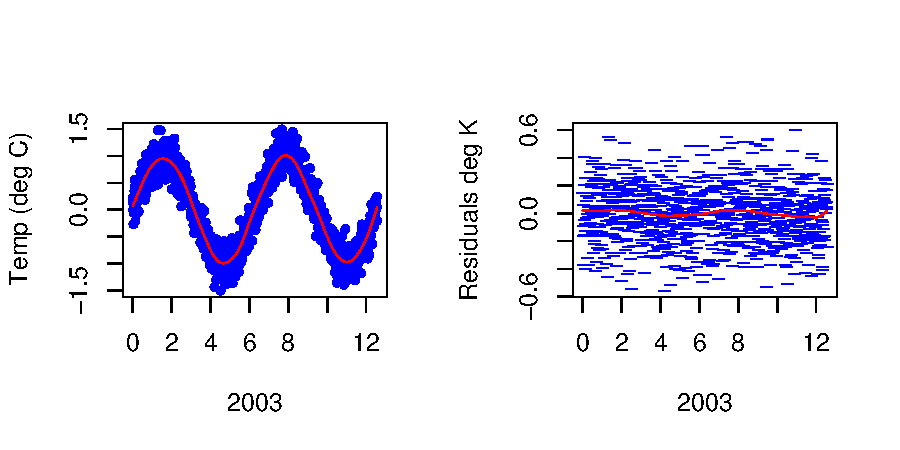
\includegraphics[width=\textwidth]{proto-smoothing10}
\caption{Smoothing of sinusoidal data (left)
and of their residuals (right)}\label{fig:smoothing10}
\end{center}
\end{figure}

\begin{figure}[h!]
\begin{center}
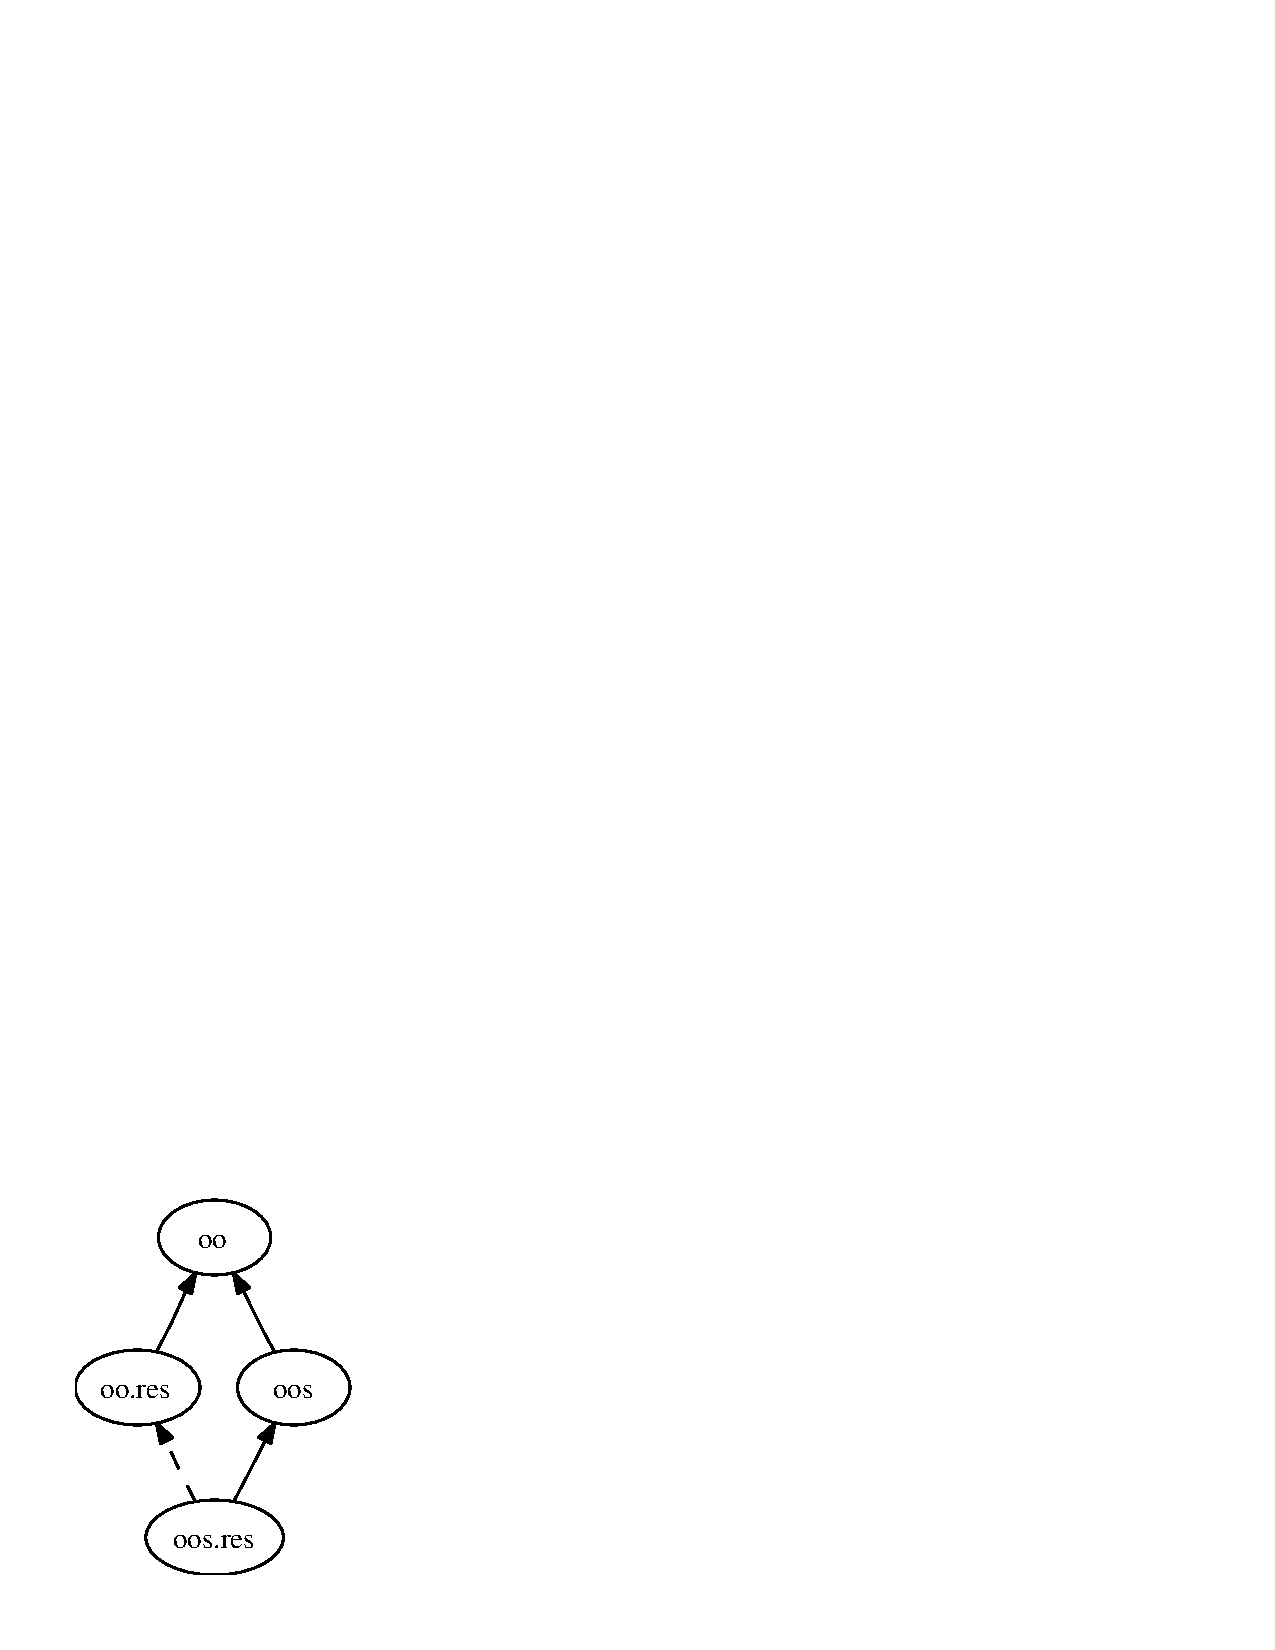
\includegraphics[width=50mm]{cloning3.pdf}
\caption{Cloning (dashed line) and delegation (solid line).  Edges point
from child to parent.}\label{fig:cloning}
\end{center}
\end{figure}

We have delegated variables
and methods and overridden both.
Thus, even with such a simple analysis, object orientation
and delegation came into play.
The reader can plainly see that smoothing and residual
analysis were not crucial to the example and this example
could be replaced with any statistical analysis including
likelihood or other estimation techniques, time series, survival
analysis, stochastic processes and so on.  The key aspect is
just that we are performing one-of analyses and do not want to
set up an elaborate class infrastructure but just want to
directly create objects to organize our calculations while
relying on delegation and dispatch to eliminate redundancy.

\subsection{Correlation, Fisher's Transform and Bootstrapping}
\label{sec:corr}

The common approach to
confidence intervals for the correlation coefficient is to
assume normality of the underlying data and then use Fisher's transform
to transform the correlation coefficient to an approximately normal
random variable.
Fisher showed that with the above normality assumption, transforming
the correlation coefficient using
the hyperbolic arc tangent function
yields a random variable
approximately distributed with an
$\frac{N(p, 1)}{\sqrt(n-3)}$ distribution.  The transformed random
variable can be used to create normal distribution confidence intervals
and the procedure can be back transformed to get confidence intervals
for the original correlation coefficient.

A more recent approach to confidence intervals for the correlation
coefficient is to use bootstrapping.  This does not require the
assumption of normality of the underlying distribution and requires
no special purpose theory devoted solely to the correlation coefficient,

Let us calculate the 95\%
confidence intervals using Fisher's transform
first.  We use \code{GNP} and \code{Unemployed} from the Longley data
set.  First we retrieve the data set and extract the required columns
into \code{x}.  Then we set \code{n} to the number of cases
and \code{pp} to the percentiles
of interest.  Finally we calculate the sample correlation and
create a function to calculate the confidence interval using
Fisher's Transform.  This function not only returns the confidence
interval but also stores it in \code{CI} in the receiver object.

\begin{Schunk}
\begin{Sinput}
> longley.ci <- proto(expr = {
+     data(longley)
+     x <- longley[, c("GNP", "Unemployed")]
+     n <- nrow(x)
+     pp <- c(0.025, 0.975)
+     corx <- cor(x)[1, 2]
+     ci <- function(.) (.$CI <- tanh(atanh(.$corx) + qnorm(.$pp)/sqrt(.$n -
+         3)))
+ })
\end{Sinput}
\end{Schunk}

Now let us repeat this analysis using the bootstrapping approach.  We
derive a new object \code{longley.ci.boot} as child of
\code{longley.ci}, setting the number of replications, \code{N}, and
defining the procedure, \code{ci} which does the actual bootstrap
calculation.

\begin{Schunk}
\begin{Sinput}
> longley.ci.boot <- longley.ci$proto({
+     N <- 1000
+     ci <- function(.) {
+         corx <- function(idx) cor(.$x[idx, ])[1, 2]
+         samp <- replicate(.$N, corx(sample(.$n, replace = TRUE)))
+         (.$CI <- quantile(samp, .$pp))
+     }
+ })
\end{Sinput}
\end{Schunk}

In the example code below the first line runs the Fisher Transform
procedure and the second runs the bootstrap procedure.  Just to check
that we have performed sufficient bootstrap iterations we rerun it in
the third line, creating a delegated object on-the-fly running its
\code{ci} method and then immediately throwing the object away.
The fact that 4,000
replications give roughly the same result as 1,000 replications
satisfies us that we have used a sufficient number of replications.

\begin{Schunk}
\begin{Sinput}
> longley.ci$ci()
\end{Sinput}
\begin{Soutput}
[1] 0.1549766 0.8464304
\end{Soutput}
\begin{Sinput}
> longley.ci.boot$ci()
\end{Sinput}
\begin{Soutput}
     2.5%     97.5%
0.2299395 0.8211854
\end{Soutput}
\begin{Sinput}
> longley.ci.boot$proto(N = 4000)$ci()
\end{Sinput}
\begin{Soutput}
     2.5%     97.5%
0.2480999 0.8259276
\end{Soutput}
\end{Schunk}

We now have the results stored in two objects nicely organized for the
future.  Note, again, that despite the simplicity of the example we
have used the features of object oriented programming, coupling the
data and methods that go together, while relying on delegation and
dispatch to avoid duplication.

\subsection{Dendrograms}
\label{sec:tree}

In \cite{Gentleman2002} there is an \proglang{S4}
example of creating a binary tree
for use as a dendrogram.  Here we directly define a binary tree with no
setup at all.  To keep it short we will create a binary tree of only
two nodes having a root whose left branch points to a leaf.  The leaf
inherits the \code{value} and \code{incr} components from the root.
The attractive feature is that the leaf be defined as a child of the
parent using \code{proto} before the parent is even finished
being defined.  Compared to the cited \proglang{S4} example where it
was necessary to create an extra class to introduce the required level of
indirection there is no need to take any similar action.

\code{tree} is the root node of the tree.  It has four components.  A
method \code{incr} which increments the \code{value} component, a
\code{..Name}, the \code{value} component itself and the left branch
\code{..left}.  \code{..left} is itself a proto object which is a
child of \code{tree}.  The leaf inherits the \code{value} component
from its parent, the root.  As mentioned, at the time we define
\code{..left} we have not even finished defining \code{tree} yet we
are able to implicitly reference the yet to be defined parent.

\begin{Schunk}
\begin{Sinput}
> tree <- proto(expr = {
+     incr <- function(., val) .$value <- .$value + val
+     ..Name <- "root"
+     value <- 3
+     ..left <- proto(expr = {
+         ..Name = "leaf"
+     })
+ })
\end{Sinput}
\end{Schunk}

Although this is a simple structure we could have embedded additional
children into \code{root} and \code{leaf} and so on recursively making
the tree or dendrogram arbitrarily complex.

Let us do some computation with this structure.  We display the
\code{value} fields in the two nodes, increment the value field in the
root and then display the two nodes again to show .that the leaf
changed too.

\begin{Schunk}
\begin{Sinput}
> cat("root:", tree$value, "leaf:", tree$..left$value, "\n")
\end{Sinput}
\begin{Soutput}
root: 3 leaf: 3
\end{Soutput}
\begin{Sinput}
> tree$incr(1)
> cat("root:", tree$value, "leaf:", tree$..left$value, "\n")
\end{Sinput}
\begin{Soutput}
root: 4 leaf: 4
\end{Soutput}
\end{Schunk}

If we increment \code{value} in \code{leaf} directly (see the example
below where we increment it by 10) then it receives its own copy of
\code{value} so from that point on \code{leaf} no longer inherits
\code{value} from \code{root}.  Thus incrementing the root by 5 no
longer increments the \code{value} field in the leaf.

\begin{Schunk}
\begin{Sinput}
> tree$..left$incr(10)
> cat("root:", tree$value, "leaf:", tree$..left$value, "\n")
\end{Sinput}
\begin{Soutput}
root: 4 leaf: 14
\end{Soutput}
\begin{Sinput}
> tree$incr(5)
> cat("root:", tree$value, "leaf:", tree$..left$value, "\n")
\end{Sinput}
\begin{Soutput}
root: 9 leaf: 14
\end{Soutput}
\end{Schunk}

\subsection{From Prototypes to Classes}
\label{sec:increment}

In many cases we will use \pkg{proto} for a design that uses prototypes
during the full development cycle.  In other cases we may use it in an
incremental way starting with prototypes but ultimately transitioning
to classes.
As shown in Section~\ref{sec:traits} the \pkg{proto} package is
powerful enough to handle class-based as well as class-free programming.
Here we illustrate this process of incremental design
starting with
concrete objects and then over time classifing them into classes,
evolving a class-based program.  \pkg{proto} provides a smooth
transition path since it can handle both the class-free and the class-based
phases -- there is no need to switch object systems part way through.
In this example, we define an object which holds a linear equation, \code{eq},
represented as a character string in terms of the unknown variable \code{x}
and a \code{print} and a \code{solve} method.  We execute the
\code{print} method
to solve it.  We also create child object \code{lineq2}
which overrides \code{eq} and execute its \code{print} method.

\begin{Schunk}
\begin{Sinput}
> lineq <- proto(eq = "6*x + 12 - 10*x/4 = 2*x", solve = function(.) {
+     e <- eval(parse(text = paste(sub("=", "-(", .$eq), ")")),
+         list(x = 0+1i))
+     -Re(e)/Im(e)
+ }, print = function(.) cat("Equation:", .$eq, "Solution:", .$solve(),
+     "\n"))
> lineq$print()
\end{Sinput}
\begin{Soutput}
Equation: 6*x + 12 - 10*x/4 = 2*x Solution: -8
\end{Soutput}
\begin{Sinput}
> lineq2 <- lineq$proto(eq = "2*x = 7*x-12+x")
> lineq2$print()
\end{Sinput}
\begin{Soutput}
Equation: 2*x = 7*x-12+x Solution: 2
\end{Soutput}
\end{Schunk}

We could continue with enhancements but at this point we decide that we
have a general case and so wish
to abstract \code{lineq} into a class.  Thus we define a trait,
\code{Lineq}, which is just \code{lineq} minus \code{eq} plus
a constructor \code{new}.  The key difference between \code{new}
and the usual \code{proto} function
is that with \code{new} the initialization of \code{eq} is mandatory.
Having completed this definition
we instantiate an object of
class/trait \code{Lineq} and execute it.

\begin{Schunk}
\begin{Sinput}
> Lineq <- lineq
> rm(eq, envir = Lineq)
> Lineq$new <- function(., eq) proto(., eq = eq)
> lineq3 <- Lineq$new("3*x=6")
> lineq3$print()
\end{Sinput}
\begin{Soutput}
Equation: 3*x=6 Solution: 2
\end{Soutput}
\end{Schunk}

Note how we have transitioned from a prototype style of programming
to a class-based style of programming all the while staying within
the \pkg{proto} framework.

\section{Summary} \label{sec:summary}

\subsection{Benefits}
\label{sec:benefits}

The key benefit of the \pkg{proto} package is to provide
access to a style of programming that has not been conveniently
accessible within \proglang{R} or any other mainstream language today.

\pkg{proto} can be used in two key ways: class-free object oriented programming
and class-based object oriented programming.

A key application for \pkg{proto} in class-free programming is to wrap the code
and data for each run of a particular statistical study into an object for
purposes of organization and reproducibility.  It provides such organization
directly and without the need and overhead of class definitions
yet still provides the
inheritance and dispatch advantages of object oriented programming.
We provide examples of this style of programming in
Section~\ref{sec:smooth}
and
Section~\ref{sec:corr}.
A third example in
Section~\ref{sec:tree} illustrates a beneficial use of \pkg{proto} with
recursive data structures.

Another situation where prototype programming is of interest is in the initial
development stages of a program.  In this case, the design may not be fully
clear so it is more convenient to create concrete objects individually rather
than premature abstractions through classes.  The \code{graph.proto}
function can be used to generate visual representations of the object
tree suggesting classifications of objects so that
as the program evolves the general case becomes clearer and
in a bottom up fashion the objects are incrementally abstracted into
classes.  In this case,
\pkg{proto} provides a smooth transition path since it not only supports
class-free programming but, as explained in the Section~\ref{sec:traits}, is
sufficiently powerful to support class-based programming, as well.


\subsection{Conclusion}
\label{sec:conclusion}

The package \pkg{proto} provides an \proglang{S3} subclass of the
\code{environment} class for constructing and manipulating object
oriented systems without classes.  It can also emulate classes even
though classes are not a primitive structure.  Its key design goals
are to provide as simple and as thin a layer as practically possible
while giving the user convenient access to this alternate object
oriented paradigm.  This paper describes, by example, how prototype
programming can be carried out in \proglang{R} using \pkg{proto} and
illustrates such usage.  Delegation, cloning traits and general
manipulation and incremental development are all reviewed by example.

\section*{Computational details}
\label{sec:compute}

The results in this paper were obtained using \proglang{R} 2.1.0 with
the package \pkg{proto} 0.3--2. \proglang{R} itself and the
\pkg{proto} package are available from CRAN at
\url{http://CRAN.R-project.org/}.  The GraphViz software is available
from \url{http://www.graphviz.org}.

\phantomsection
\addcontentsline{toc}{section}{References}
\bibliography{proto}
%\input{proto.bbl}

\newpage\mbox{}
\begin{appendix}
\section{Frequently Asked Questions}
\label{sec:faq}
\begin{enumerate}
\item{What scope do unqualified object references within methods use?

A \pkg{proto} object is an environment and that environment
is the environment
of the methods in it (by default).
That is, unqualified object references
within a \pkg{proto} method look first in the method itself and secondly in the
\pkg{proto} object containing the method.
This is referred to as object
scope as opposed to lexical scope or dynamic scope.  It allows simple
situations, where delegation is not used, to use unqualified names.  Thus
simple situations remain simple.
\citep{Kates2004}
discusses the fragile base class problem which
relates to this question. Also note that if a \pkg{proto} object is created
via the \code{proto} function using an argument of \code{funEnvir = FALSE}
then the environment of the function/method will not be set as just
described (but rather it will retain its original environment) so the
above does not apply.  This can be used for instances when non-default
processing is desirable.}
\item{Why does \code{obj\$meth} not return the method, \code{meth}?

Conceptually \code{obj\$meth} returns \code{meth} but with
\code{obj} already inserted into its first argument.
This is termed an instantiated
\pkg{proto}
method and is of \proglang{S3} class \code{"instantiatedProtoMethod"}.

In contrast, the method itself (i.e. the uninstantited method)
would not have the first argument already
inserted.  To return the method itself use \code{with(obj, meth}.

The main advantage of a design that makes the distinction between instantiated
and uninstantiated methods is that uninstantiated methods are never
changed so
debugging can be more readily carried out (as discussed in the next
question and answer).
}
\item{How does one debug a method?

\pkg{proto} does not dynamically redefine methods.  This has the advantage
that the ordinary \proglang{R} \code{debug} and \code{undebug} commands can be
used.  When using these be sure that to use them with the uninstantiated method
itself and not the instantiated method derived from it.  That is,
use:
\begin{verbatim}
   with(obj, debug(meth))
\end{verbatim}

and not
\begin{verbatim}
   debug(obj$meth) # wrong
\end{verbatim}
}
\item{Is multiple inheritance supported?

No. \pkg{proto} is just a thin layer on top of \proglang{R}
environments and \proglang{R} environments
provide single inheritance only.  \citep{Kates2004}
discusses some ways of handling situations which would otherwise require
multiple inheritance.}
\item{Does \pkg{proto} support lazy evaluation?

Since \code{proto} methods are just \proglang{R} functions they do support
lazy evaluation; however, the \code{proto} function itself
does evaluate its arguments.  To get the
effect of lazy evaluation when using the \code{proto}
function replace any properties with a function.

If the caller is the parent of the \code{proto} object then its
particularly simple.  Note how we got the equivalent of lazy evaluation
in the second example where f is a function:

\begin{verbatim}
# eager evaluation
x <- 0
p <- proto(f = x, g = function(.) $x)
x <- 1
p$f # 0

# versus making f a function

# simulates lazy evaluation
x <- 0
p <- proto(f = function(.) x, g = function(.) .$x)
x <- 1
p$f() # 1
\end{verbatim}

If we cannot guarantee that the proto object has the caller
as its parent then ensure that the environment of the function
has not been reset.  If no method needs to reference \code{.that}
or \code{.super} then we can arrange for that using
\code{funEnvir=FALSE} as seen here in the second example:
\begin{verbatim}

# does not work as intended
x <- 0
p <- proto(x = 99)
q <- p$proto(f = function(.) x, g = function(.) .$x)
x <- 1
q$f() # 99

# does work
x <- 0
p <- proto(x = 99)
q <- p$proto(f = function(.) x, g = function(.) .$x, funEnvir = FALSE)
x <- 1
q$f() # 1
\end{verbatim}

If we wish only to not reset the function used to simulate
lazy evaluation then we can do it using either of the
two equivalent alternatives below.  \code{g}
is an ordinary method whose environment is reset to \code{q}
whereas \code{f} is a function whose environment is not reset and
serves to provide lazy evaluation for \code{x} found in the caller.

\begin{verbatim}
x <- 0
p <- proto(x = 99)
# g will use q's y in children of q even if those children
# override y
q <- p$proto(y = 25, g = function(.) .that$y + .$x)
q[["f"]] <- function(.) x
x <- 1
q$f() # 1

# equivalent alternative

x <- 0
p <- proto(x = 99)
q <- proto(f = function(.) x, funEnvir = FALSE,
	envir = p$proto(y = 25, g = function(.) .that$y + .$x))
x <- 1
q$f() # 1
\end{verbatim}
}
\end{enumerate}
\newpage{}
\section{Reference Card}
\label{sec:ref}
\input{protoref-raw}
\end{appendix}

\end{document}



\newpage\mbox{}
\begin{appendix}
\section{Frequently Asked Questions}
\label{sec:faq}
\begin{enumerate}
\item{What scope do unqualified object references within methods use?

A \pkg{proto} object is an environment and that environment
is the environment
of the methods in it (by default).
That is, unqualified object references
within a \pkg{proto} method look first in the method itself and secondly in the
\pkg{proto} object containing the method.
This is referred to as object
scope as opposed to lexical scope or dynamic scope.  It allows simple
situations, where delegation is not used, to use unqualified names.  Thus
simple situations remain simple.
\citep{Kates2004}
discusses the fragile base class problem which
relates to this question. Also note that if a \pkg{proto} object is created
via the \code{proto} function using an argument of \code{funEnvir = FALSE}
then the environment of the function/method will not be set as just
described (but rather it will retain its original environment) so the
above does not apply.  This can be used for instances when non-default
processing is desirable.}
\item{Why does \code{obj\$meth} not return the method, \code{meth}?

Conceptually \code{obj\$meth} returns \code{meth} but with
\code{obj} already inserted into its first argument.
This is termed an instantiated
\pkg{proto}
method and is of \proglang{S3} class \code{"instantiatedProtoMethod"}.

In contrast, the method itself (i.e. the uninstantited method)
would not have the first argument already
inserted.  To return the method itself use \code{with(obj, meth}.

The main advantage of a design that makes the distinction between instantiated
and uninstantiated methods is that uninstantiated methods are never
changed so
debugging can be more readily carried out (as discussed in the next
question and answer).
}
\item{How does one debug a method?

\pkg{proto} does not dynamically redefine methods.  This has the advantage
that the ordinary \proglang{R} \code{debug} and \code{undebug} commands can be
used.  When using these be sure that to use them with the uninstantiated method
itself and not the instantiated method derived from it.  That is,
use:
\begin{verbatim}
   with(obj, debug(meth))
\end{verbatim}

and not
\begin{verbatim}
   debug(obj$meth) # wrong
\end{verbatim}
}
\item{Is multiple inheritance supported?

No. \pkg{proto} is just a thin layer on top of \proglang{R}
environments and \proglang{R} environments
provide single inheritance only.  \citep{Kates2004}
discusses some ways of handling situations which would otherwise require
multiple inheritance.}
\item{Does \pkg{proto} support lazy evaluation?

Since \code{proto} methods are just \proglang{R} functions they do support
lazy evaluation; however, the \code{proto} function itself
does evaluate its arguments.  To get the
effect of lazy evaluation when using the \code{proto}
function replace any properties with a function.

If the caller is the parent of the \code{proto} object then its
particularly simple.  Note how we got the equivalent of lazy evaluation
in the second example where f is a function:

\begin{verbatim}
# eager evaluation
x <- 0
p <- proto(f = x, g = function(.) $x)
x <- 1
p$f # 0

# versus making f a function

# simulates lazy evaluation
x <- 0
p <- proto(f = function(.) x, g = function(.) .$x)
x <- 1
p$f() # 1
\end{verbatim}

If we cannot guarantee that the proto object has the caller
as its parent then ensure that the environment of the function
has not been reset.  If no method needs to reference \code{.that}
or \code{.super} then we can arrange for that using
\code{funEnvir=FALSE} as seen here in the second example:
\begin{verbatim}

# does not work as intended
x <- 0
p <- proto(x = 99)
q <- p$proto(f = function(.) x, g = function(.) .$x)
x <- 1
q$f() # 99

# does work
x <- 0
p <- proto(x = 99)
q <- p$proto(f = function(.) x, g = function(.) .$x, funEnvir = FALSE)
x <- 1
q$f() # 1
\end{verbatim}

If we wish only to not reset the function used to simulate
lazy evaluation then we can do it using either of the
two equivalent alternatives below.  \code{g}
is an ordinary method whose environment is reset to \code{q}
whereas \code{f} is a function whose environment is not reset and
serves to provide lazy evaluation for \code{x} found in the caller.

\begin{verbatim}
x <- 0
p <- proto(x = 99)
# g will use q's y in children of q even if those children
# override y
q <- p$proto(y = 25, g = function(.) .that$y + .$x)
q[["f"]] <- function(.) x
x <- 1
q$f() # 1

# equivalent alternative

x <- 0
p <- proto(x = 99)
q <- proto(f = function(.) x, funEnvir = FALSE,
	envir = p$proto(y = 25, g = function(.) .that$y + .$x))
x <- 1
q$f() # 1
\end{verbatim}
}
\end{enumerate}
\newpage{}
\section{Reference Card}
\label{sec:ref}
\begin{tabular}{rp{10.5cm}}
\multicolumn{2}{l}{\textbf{Creation}} \\
\code{proto} & \code{proto(., expr, envir, ... )}  embeds the components
  specified in \code{expr} and/or \code{...} into the \code{proto} object
  or environment specified by \code{envir}.  A new object is created if
  \code{envir} is omitted.  The parent of the object is set to \code{.} .
  The parent object, \code{.}, defaults
  to the parent of \code{envir} or the current environment if \code{envir}
  is missing. \code{expr} and \code{\dots} default
  to empty specifications.
  The returned object will contain \code{.that} and \code{.super} variables
  referring to the object itself and the parent of the object, respectively.
  \\[0.5cm]

\multicolumn{2}{l}{\textbf{Coercion}} \\
  \code{as.proto} & If \code{x} is a \code{proto} object or environment
  then \code{x} is returned as a \code{proto} object
  with the values of \code{.that} and \code{.super} inserted in the case
  of an environment or refreshed in the case of a proto object.
  If \code{x} is a list then additional arguments are available:
  \code{as.proto(x, envir, parent, FUN, all.names, ...)}.  
  Each component of \code{x} is copied into \code{envir}.  
  \code{envir} may be an \code{environment} or \code{proto} object.
  If it is missing a new \code{proto} object is created.  
  If \code{all.names = FALSE} then only list components whose
  names do not begin with a dot are copied.  If \code{FUN} is specified
  then, in addition, only list components \code{v} for which \code{FUN(v)}
  is \code{TRUE} are copied.  If \code{parent} is specified then the
  resulting \code{proto} object will have that parent.  Otherwise, it
  will have the parent of \code{envir} if \code{envir} was specified.
  If neither are specified the parent defaults to the current environment.
  \\[0.5cm]

\multicolumn{2}{l}{\textbf{Standard methods}} \\
\code{\$} & \code{obj\$x} searches \code{proto} object \code{obj} for
  \code{x}.  If the name \code{x} does not begin with two dots then
  ancestors are searched if the name is not found in \code{obj}.
  If \code{x} is a variable
  or if \code{obj} is \code{.super} or \code{.that} then \code{x} is returned.
  Otherwise, the call \code{obj\$x(...)} is
  equivalent to the call \code{get("x", obj)(obj, ...)}. If it is desired
  to return a method as a value  rather than in 
  the context of a call then use \code{get("x", obj)} (or \code{obj[["x"]]}
  \code{x} is known to be directly in \code{obj})
  rather than \code{\$} syntax.\\
\code{\$<-} & \code{obj\$x <- value} sets \code{x} in \code{proto} object
  \code{obj} to \code{value} creating \code{x} if not present.  If 
  \code{obj} is \code{.super} then a side effect is to set the parent
  of \code{obj} to \code{value}.\\
\code{is.proto(x)} & returns \code{TRUE} if \code{x} is a \code{proto}
  object and othewise returns \code{FALSE}.\\[0.5cm]

\multicolumn{2}{l}{\textbf{Utilities}} \\
\code{graph.proto} & \code{graph.proto(e, g, child.to.parent)} adds a
  graph in the sense of the \code{graph} package representing an ancestor tree
  among all \code{proto} objects in \code{environment} or \code{proto} 
  object \code{e} to graph \code{g}.
  \code{e} defaults to the current environment and \code{g}
  defaults to an empty graph.
  \code{child.to.parent} is a logical variable specifying the direction
   of arrows.  By default they are displayed from children to parents.
  \\[0.5cm]
\end{tabular}

\end{appendix}

\end{document}



\newpage\mbox{}
\begin{appendix}
\section{Frequently Asked Questions}
\label{sec:faq}
\begin{enumerate}
\item{What scope do unqualified object references within methods use?

A \pkg{proto} object is an environment and that environment
is the environment
of the methods in it (by default).
That is, unqualified object references
within a \pkg{proto} method look first in the method itself and secondly in the
\pkg{proto} object containing the method.
This is referred to as object
scope as opposed to lexical scope or dynamic scope.  It allows simple
situations, where delegation is not used, to use unqualified names.  Thus
simple situations remain simple.
\citep{Kates2004}
discusses the fragile base class problem which
relates to this question. Also note that if a \pkg{proto} object is created
via the \code{proto} function using an argument of \code{funEnvir = FALSE}
then the environment of the function/method will not be set as just
described (but rather it will retain its original environment) so the
above does not apply.  This can be used for instances when non-default
processing is desirable.}
\item{Why does \code{obj\$meth} not return the method, \code{meth}?

Conceptually \code{obj\$meth} returns \code{meth} but with
\code{obj} already inserted into its first argument.
This is termed an instantiated
\pkg{proto}
method and is of \proglang{S3} class \code{"instantiatedProtoMethod"}.

In contrast, the method itself (i.e. the uninstantited method)
would not have the first argument already
inserted.  To return the method itself use \code{with(obj, meth}.

The main advantage of a design that makes the distinction between instantiated
and uninstantiated methods is that uninstantiated methods are never
changed so
debugging can be more readily carried out (as discussed in the next
question and answer).
}
\item{How does one debug a method?

\pkg{proto} does not dynamically redefine methods.  This has the advantage
that the ordinary \proglang{R} \code{debug} and \code{undebug} commands can be
used.  When using these be sure that to use them with the uninstantiated method
itself and not the instantiated method derived from it.  That is,
use:
\begin{verbatim}
   with(obj, debug(meth))
\end{verbatim}

and not
\begin{verbatim}
   debug(obj$meth) # wrong
\end{verbatim}
}
\item{Is multiple inheritance supported?

No. \pkg{proto} is just a thin layer on top of \proglang{R}
environments and \proglang{R} environments
provide single inheritance only.  \citep{Kates2004}
discusses some ways of handling situations which would otherwise require
multiple inheritance.}
\item{Does \pkg{proto} support lazy evaluation?

Since \code{proto} methods are just \proglang{R} functions they do support
lazy evaluation; however, the \code{proto} function itself
does evaluate its arguments.  To get the
effect of lazy evaluation when using the \code{proto}
function replace any properties with a function.

If the caller is the parent of the \code{proto} object then its
particularly simple.  Note how we got the equivalent of lazy evaluation
in the second example where f is a function:

\begin{verbatim}
# eager evaluation
x <- 0
p <- proto(f = x, g = function(.) $x)
x <- 1
p$f # 0

# versus making f a function

# simulates lazy evaluation
x <- 0
p <- proto(f = function(.) x, g = function(.) .$x)
x <- 1
p$f() # 1
\end{verbatim}

If we cannot guarantee that the proto object has the caller
as its parent then ensure that the environment of the function
has not been reset.  If no method needs to reference \code{.that}
or \code{.super} then we can arrange for that using
\code{funEnvir=FALSE} as seen here in the second example:
\begin{verbatim}

# does not work as intended
x <- 0
p <- proto(x = 99)
q <- p$proto(f = function(.) x, g = function(.) .$x)
x <- 1
q$f() # 99

# does work
x <- 0
p <- proto(x = 99)
q <- p$proto(f = function(.) x, g = function(.) .$x, funEnvir = FALSE)
x <- 1
q$f() # 1
\end{verbatim}

If we wish only to not reset the function used to simulate
lazy evaluation then we can do it using either of the
two equivalent alternatives below.  \code{g}
is an ordinary method whose environment is reset to \code{q}
whereas \code{f} is a function whose environment is not reset and
serves to provide lazy evaluation for \code{x} found in the caller.

\begin{verbatim}
x <- 0
p <- proto(x = 99)
# g will use q's y in children of q even if those children
# override y
q <- p$proto(y = 25, g = function(.) .that$y + .$x)
q[["f"]] <- function(.) x
x <- 1
q$f() # 1

# equivalent alternative

x <- 0
p <- proto(x = 99)
q <- proto(f = function(.) x, funEnvir = FALSE,
	envir = p$proto(y = 25, g = function(.) .that$y + .$x))
x <- 1
q$f() # 1
\end{verbatim}
}
\end{enumerate}
\newpage{}
\section{Reference Card}
\label{sec:ref}
\begin{tabular}{rp{10.5cm}}
\multicolumn{2}{l}{\textbf{Creation}} \\
\code{proto} & \code{proto(., expr, envir, ... )}  embeds the components
  specified in \code{expr} and/or \code{...} into the \code{proto} object
  or environment specified by \code{envir}.  A new object is created if
  \code{envir} is omitted.  The parent of the object is set to \code{.} .
  The parent object, \code{.}, defaults
  to the parent of \code{envir} or the current environment if \code{envir}
  is missing. \code{expr} and \code{\dots} default
  to empty specifications.
  The returned object will contain \code{.that} and \code{.super} variables
  referring to the object itself and the parent of the object, respectively.
  \\[0.5cm]

\multicolumn{2}{l}{\textbf{Coercion}} \\
  \code{as.proto} & If \code{x} is a \code{proto} object or environment
  then \code{x} is returned as a \code{proto} object
  with the values of \code{.that} and \code{.super} inserted in the case
  of an environment or refreshed in the case of a proto object.
  If \code{x} is a list then additional arguments are available:
  \code{as.proto(x, envir, parent, FUN, all.names, ...)}.  
  Each component of \code{x} is copied into \code{envir}.  
  \code{envir} may be an \code{environment} or \code{proto} object.
  If it is missing a new \code{proto} object is created.  
  If \code{all.names = FALSE} then only list components whose
  names do not begin with a dot are copied.  If \code{FUN} is specified
  then, in addition, only list components \code{v} for which \code{FUN(v)}
  is \code{TRUE} are copied.  If \code{parent} is specified then the
  resulting \code{proto} object will have that parent.  Otherwise, it
  will have the parent of \code{envir} if \code{envir} was specified.
  If neither are specified the parent defaults to the current environment.
  \\[0.5cm]

\multicolumn{2}{l}{\textbf{Standard methods}} \\
\code{\$} & \code{obj\$x} searches \code{proto} object \code{obj} for
  \code{x}.  If the name \code{x} does not begin with two dots then
  ancestors are searched if the name is not found in \code{obj}.
  If \code{x} is a variable
  or if \code{obj} is \code{.super} or \code{.that} then \code{x} is returned.
  Otherwise, the call \code{obj\$x(...)} is
  equivalent to the call \code{get("x", obj)(obj, ...)}. If it is desired
  to return a method as a value  rather than in 
  the context of a call then use \code{get("x", obj)} (or \code{obj[["x"]]}
  \code{x} is known to be directly in \code{obj})
  rather than \code{\$} syntax.\\
\code{\$<-} & \code{obj\$x <- value} sets \code{x} in \code{proto} object
  \code{obj} to \code{value} creating \code{x} if not present.  If 
  \code{obj} is \code{.super} then a side effect is to set the parent
  of \code{obj} to \code{value}.\\
\code{is.proto(x)} & returns \code{TRUE} if \code{x} is a \code{proto}
  object and othewise returns \code{FALSE}.\\[0.5cm]

\multicolumn{2}{l}{\textbf{Utilities}} \\
\code{graph.proto} & \code{graph.proto(e, g, child.to.parent)} adds a
  graph in the sense of the \code{graph} package representing an ancestor tree
  among all \code{proto} objects in \code{environment} or \code{proto} 
  object \code{e} to graph \code{g}.
  \code{e} defaults to the current environment and \code{g}
  defaults to an empty graph.
  \code{child.to.parent} is a logical variable specifying the direction
   of arrows.  By default they are displayed from children to parents.
  \\[0.5cm]
\end{tabular}

\end{appendix}

\end{document}



\newpage\mbox{}
\begin{appendix}
\section{Frequently Asked Questions}
\label{sec:faq}
\begin{enumerate}
\item{What scope do unqualified object references within methods use?

A \pkg{proto} object is an environment and that environment
is the environment
of the methods in it (by default).
That is, unqualified object references
within a \pkg{proto} method look first in the method itself and secondly in the
\pkg{proto} object containing the method.
This is referred to as object
scope as opposed to lexical scope or dynamic scope.  It allows simple
situations, where delegation is not used, to use unqualified names.  Thus
simple situations remain simple.
\citep{Kates2004}
discusses the fragile base class problem which
relates to this question. Also note that if a \pkg{proto} object is created
via the \code{proto} function using an argument of \code{funEnvir = FALSE}
then the environment of the function/method will not be set as just
described (but rather it will retain its original environment) so the
above does not apply.  This can be used for instances when non-default
processing is desirable.}
\item{Why does \code{obj\$meth} not return the method, \code{meth}?

Conceptually \code{obj\$meth} returns \code{meth} but with
\code{obj} already inserted into its first argument.
This is termed an instantiated
\pkg{proto}
method and is of \proglang{S3} class \code{"instantiatedProtoMethod"}.

In contrast, the method itself (i.e. the uninstantited method)
would not have the first argument already
inserted.  To return the method itself use \code{with(obj, meth}.

The main advantage of a design that makes the distinction between instantiated
and uninstantiated methods is that uninstantiated methods are never
changed so
debugging can be more readily carried out (as discussed in the next
question and answer).
}
\item{How does one debug a method?

\pkg{proto} does not dynamically redefine methods.  This has the advantage
that the ordinary \proglang{R} \code{debug} and \code{undebug} commands can be
used.  When using these be sure that to use them with the uninstantiated method
itself and not the instantiated method derived from it.  That is,
use:
\begin{verbatim}
   with(obj, debug(meth))
\end{verbatim}

and not
\begin{verbatim}
   debug(obj$meth) # wrong
\end{verbatim}
}
\item{Is multiple inheritance supported?

No. \pkg{proto} is just a thin layer on top of \proglang{R}
environments and \proglang{R} environments
provide single inheritance only.  \citep{Kates2004}
discusses some ways of handling situations which would otherwise require
multiple inheritance.}
\item{Does \pkg{proto} support lazy evaluation?

Since \code{proto} methods are just \proglang{R} functions they do support
lazy evaluation; however, the \code{proto} function itself
does evaluate its arguments.  To get the
effect of lazy evaluation when using the \code{proto}
function replace any properties with a function.

If the caller is the parent of the \code{proto} object then its
particularly simple.  Note how we got the equivalent of lazy evaluation
in the second example where f is a function:

\begin{verbatim}
# eager evaluation
x <- 0
p <- proto(f = x, g = function(.) $x)
x <- 1
p$f # 0

# versus making f a function

# simulates lazy evaluation
x <- 0
p <- proto(f = function(.) x, g = function(.) .$x)
x <- 1
p$f() # 1
\end{verbatim}

If we cannot guarantee that the proto object has the caller
as its parent then ensure that the environment of the function
has not been reset.  If no method needs to reference \code{.that}
or \code{.super} then we can arrange for that using
\code{funEnvir=FALSE} as seen here in the second example:
\begin{verbatim}

# does not work as intended
x <- 0
p <- proto(x = 99)
q <- p$proto(f = function(.) x, g = function(.) .$x)
x <- 1
q$f() # 99

# does work
x <- 0
p <- proto(x = 99)
q <- p$proto(f = function(.) x, g = function(.) .$x, funEnvir = FALSE)
x <- 1
q$f() # 1
\end{verbatim}

If we wish only to not reset the function used to simulate
lazy evaluation then we can do it using either of the
two equivalent alternatives below.  \code{g}
is an ordinary method whose environment is reset to \code{q}
whereas \code{f} is a function whose environment is not reset and
serves to provide lazy evaluation for \code{x} found in the caller.

\begin{verbatim}
x <- 0
p <- proto(x = 99)
# g will use q's y in children of q even if those children
# override y
q <- p$proto(y = 25, g = function(.) .that$y + .$x)
q[["f"]] <- function(.) x
x <- 1
q$f() # 1

# equivalent alternative

x <- 0
p <- proto(x = 99)
q <- proto(f = function(.) x, funEnvir = FALSE,
	envir = p$proto(y = 25, g = function(.) .that$y + .$x))
x <- 1
q$f() # 1
\end{verbatim}
}
\end{enumerate}
\newpage{}
\section{Reference Card}
\label{sec:ref}
\begin{tabular}{rp{10.5cm}}
\multicolumn{2}{l}{\textbf{Creation}} \\
\code{proto} & \code{proto(., expr, envir, ... )}  embeds the components
  specified in \code{expr} and/or \code{...} into the \code{proto} object
  or environment specified by \code{envir}.  A new object is created if
  \code{envir} is omitted.  The parent of the object is set to \code{.} .
  The parent object, \code{.}, defaults
  to the parent of \code{envir} or the current environment if \code{envir}
  is missing. \code{expr} and \code{\dots} default
  to empty specifications.
  The returned object will contain \code{.that} and \code{.super} variables
  referring to the object itself and the parent of the object, respectively.
  \\[0.5cm]

\multicolumn{2}{l}{\textbf{Coercion}} \\
  \code{as.proto} & If \code{x} is a \code{proto} object or environment
  then \code{x} is returned as a \code{proto} object
  with the values of \code{.that} and \code{.super} inserted in the case
  of an environment or refreshed in the case of a proto object.
  If \code{x} is a list then additional arguments are available:
  \code{as.proto(x, envir, parent, FUN, all.names, ...)}.  
  Each component of \code{x} is copied into \code{envir}.  
  \code{envir} may be an \code{environment} or \code{proto} object.
  If it is missing a new \code{proto} object is created.  
  If \code{all.names = FALSE} then only list components whose
  names do not begin with a dot are copied.  If \code{FUN} is specified
  then, in addition, only list components \code{v} for which \code{FUN(v)}
  is \code{TRUE} are copied.  If \code{parent} is specified then the
  resulting \code{proto} object will have that parent.  Otherwise, it
  will have the parent of \code{envir} if \code{envir} was specified.
  If neither are specified the parent defaults to the current environment.
  \\[0.5cm]

\multicolumn{2}{l}{\textbf{Standard methods}} \\
\code{\$} & \code{obj\$x} searches \code{proto} object \code{obj} for
  \code{x}.  If the name \code{x} does not begin with two dots then
  ancestors are searched if the name is not found in \code{obj}.
  If \code{x} is a variable
  or if \code{obj} is \code{.super} or \code{.that} then \code{x} is returned.
  Otherwise, the call \code{obj\$x(...)} is
  equivalent to the call \code{get("x", obj)(obj, ...)}. If it is desired
  to return a method as a value  rather than in 
  the context of a call then use \code{get("x", obj)} (or \code{obj[["x"]]}
  \code{x} is known to be directly in \code{obj})
  rather than \code{\$} syntax.\\
\code{\$<-} & \code{obj\$x <- value} sets \code{x} in \code{proto} object
  \code{obj} to \code{value} creating \code{x} if not present.  If 
  \code{obj} is \code{.super} then a side effect is to set the parent
  of \code{obj} to \code{value}.\\
\code{is.proto(x)} & returns \code{TRUE} if \code{x} is a \code{proto}
  object and othewise returns \code{FALSE}.\\[0.5cm]

\multicolumn{2}{l}{\textbf{Utilities}} \\
\code{graph.proto} & \code{graph.proto(e, g, child.to.parent)} adds a
  graph in the sense of the \code{graph} package representing an ancestor tree
  among all \code{proto} objects in \code{environment} or \code{proto} 
  object \code{e} to graph \code{g}.
  \code{e} defaults to the current environment and \code{g}
  defaults to an empty graph.
  \code{child.to.parent} is a logical variable specifying the direction
   of arrows.  By default they are displayed from children to parents.
  \\[0.5cm]
\end{tabular}

\end{appendix}

\end{document}

